\documentclass[twoside]{book}

% Packages required by doxygen
\usepackage{fixltx2e}
\usepackage{calc}
\usepackage{doxygen}
\usepackage[export]{adjustbox} % also loads graphicx
\usepackage{graphicx}
\usepackage[utf8]{inputenc}
\usepackage{makeidx}
\usepackage{multicol}
\usepackage{multirow}
\PassOptionsToPackage{warn}{textcomp}
\usepackage{textcomp}
\usepackage[nointegrals]{wasysym}
\usepackage[table]{xcolor}

% Font selection
\usepackage[T1]{fontenc}
\usepackage[scaled=.90]{helvet}
\usepackage{courier}
\usepackage{amssymb}
\usepackage{sectsty}
\renewcommand{\familydefault}{\sfdefault}
\allsectionsfont{%
  \fontseries{bc}\selectfont%
  \color{darkgray}%
}
\renewcommand{\DoxyLabelFont}{%
  \fontseries{bc}\selectfont%
  \color{darkgray}%
}
\newcommand{\+}{\discretionary{\mbox{\scriptsize$\hookleftarrow$}}{}{}}

% Page & text layout
\usepackage{geometry}
\geometry{%
  a4paper,%
  top=2.5cm,%
  bottom=2.5cm,%
  left=2.5cm,%
  right=2.5cm%
}
\tolerance=750
\hfuzz=15pt
\hbadness=750
\setlength{\emergencystretch}{15pt}
\setlength{\parindent}{0cm}
\setlength{\parskip}{0.2cm}
\makeatletter
\renewcommand{\paragraph}{%
  \@startsection{paragraph}{4}{0ex}{-1.0ex}{1.0ex}{%
    \normalfont\normalsize\bfseries\SS@parafont%
  }%
}
\renewcommand{\subparagraph}{%
  \@startsection{subparagraph}{5}{0ex}{-1.0ex}{1.0ex}{%
    \normalfont\normalsize\bfseries\SS@subparafont%
  }%
}
\makeatother

% Headers & footers
\usepackage{fancyhdr}
\pagestyle{fancyplain}
\fancyhead[LE]{\fancyplain{}{\bfseries\thepage}}
\fancyhead[CE]{\fancyplain{}{}}
\fancyhead[RE]{\fancyplain{}{\bfseries\leftmark}}
\fancyhead[LO]{\fancyplain{}{\bfseries\rightmark}}
\fancyhead[CO]{\fancyplain{}{}}
\fancyhead[RO]{\fancyplain{}{\bfseries\thepage}}
\fancyfoot[LE]{\fancyplain{}{}}
\fancyfoot[CE]{\fancyplain{}{}}
\fancyfoot[RE]{\fancyplain{}{\bfseries\scriptsize Generated on Wed May 20 2015 11\+:20\+:36 for Video Anonymizer by Doxygen }}
\fancyfoot[LO]{\fancyplain{}{\bfseries\scriptsize Generated on Wed May 20 2015 11\+:20\+:36 for Video Anonymizer by Doxygen }}
\fancyfoot[CO]{\fancyplain{}{}}
\fancyfoot[RO]{\fancyplain{}{}}
\renewcommand{\footrulewidth}{0.4pt}
\renewcommand{\chaptermark}[1]{%
  \markboth{#1}{}%
}
\renewcommand{\sectionmark}[1]{%
  \markright{\thesection\ #1}%
}

% Indices & bibliography
\usepackage{natbib}
\usepackage[titles]{tocloft}
\setcounter{tocdepth}{3}
\setcounter{secnumdepth}{5}
\makeindex

% Hyperlinks (required, but should be loaded last)
\usepackage{ifpdf}
\ifpdf
  \usepackage[pdftex,pagebackref=true]{hyperref}
\else
  \usepackage[ps2pdf,pagebackref=true]{hyperref}
\fi
\hypersetup{%
  colorlinks=true,%
  linkcolor=blue,%
  citecolor=blue,%
  unicode%
}

% Custom commands
\newcommand{\clearemptydoublepage}{%
  \newpage{\pagestyle{empty}\cleardoublepage}%
}


%===== C O N T E N T S =====

\begin{document}

% Titlepage & ToC
\hypersetup{pageanchor=false,
             bookmarks=true,
             bookmarksnumbered=true,
             pdfencoding=unicode
            }
\pagenumbering{roman}
\begin{titlepage}
\vspace*{7cm}
\begin{center}%
{\Large Video Anonymizer }\\
\vspace*{1cm}
{\large Generated by Doxygen 1.8.9.1}\\
\vspace*{0.5cm}
{\small Wed May 20 2015 11:20:36}\\
\end{center}
\end{titlepage}
\clearemptydoublepage
\tableofcontents
\clearemptydoublepage
\pagenumbering{arabic}
\hypersetup{pageanchor=true}

%--- Begin generated contents ---
\chapter{Hierarchical Index}
\section{Class Hierarchy}
This inheritance list is sorted roughly, but not completely, alphabetically\+:\begin{DoxyCompactList}
\item \contentsline{section}{A\+V\+Writer}{\pageref{classAVWriter}}{}
\item \contentsline{section}{Characteristics}{\pageref{structCharacteristics}}{}
\item \contentsline{section}{Colors}{\pageref{classColors}}{}
\item exception\begin{DoxyCompactList}
\item \contentsline{section}{Open\+Exception}{\pageref{structOpenException}}{}
\item \contentsline{section}{Output\+Exception}{\pageref{structOutputException}}{}
\item \contentsline{section}{User\+Canceled\+Exception}{\pageref{structUserCanceledException}}{}
\item \contentsline{section}{User\+Canceled\+Opening\+Exception}{\pageref{structUserCanceledOpeningException}}{}
\end{DoxyCompactList}
\item \contentsline{section}{F\+Fmpeg\+Player}{\pageref{classFFmpegPlayer}}{}
\item \contentsline{section}{Object\+Color}{\pageref{structObjectColor}}{}
\item \contentsline{section}{Object\+Shape}{\pageref{structObjectShape}}{}
\item Q\+Label\begin{DoxyCompactList}
\item \contentsline{section}{Image\+Label}{\pageref{classImageLabel}}{}
\item \contentsline{section}{Time\+Label}{\pageref{classTimeLabel}}{}
\end{DoxyCompactList}
\item Q\+Main\+Window\begin{DoxyCompactList}
\item \contentsline{section}{Main\+Window}{\pageref{classMainWindow}}{}
\end{DoxyCompactList}
\item Q\+Slider\begin{DoxyCompactList}
\item \contentsline{section}{Player\+Slider}{\pageref{classPlayerSlider}}{}
\end{DoxyCompactList}
\item Q\+Text\+Browser\begin{DoxyCompactList}
\item \contentsline{section}{Help\+Browser}{\pageref{classHelpBrowser}}{}
\end{DoxyCompactList}
\item Q\+Widget\begin{DoxyCompactList}
\item \contentsline{section}{Anchor\+Item}{\pageref{classAnchorItem}}{}
\item \contentsline{section}{Trajectory\+Item}{\pageref{classTrajectoryItem}}{}
\item \contentsline{section}{Video\+Widget}{\pageref{classVideoWidget}}{}
\end{DoxyCompactList}
\item \contentsline{section}{Selection}{\pageref{structSelection}}{}
\item \contentsline{section}{Time\+Conversion\+:\+:Time}{\pageref{structTimeConversion_1_1Time}}{}
\item \contentsline{section}{Tracked\+Object}{\pageref{classTrackedObject}}{}
\item \contentsline{section}{Tracking\+Algorithm}{\pageref{classTrackingAlgorithm}}{}
\item \contentsline{section}{Trajectory\+Entry}{\pageref{structTrajectoryEntry}}{}
\item \contentsline{section}{Trajectory\+Section}{\pageref{structTrajectorySection}}{}
\item \contentsline{section}{Video\+Frame}{\pageref{classVideoFrame}}{}
\item \contentsline{section}{Video\+Tracker}{\pageref{classVideoTracker}}{}
\end{DoxyCompactList}

\chapter{Class Index}
\section{Class List}
Here are the classes, structs, unions and interfaces with brief descriptions\+:\begin{DoxyCompactList}
\item\contentsline{section}{\hyperlink{classAnchorItem}{Anchor\+Item} }{\pageref{classAnchorItem}}{}
\item\contentsline{section}{\hyperlink{classAVWriter}{A\+V\+Writer} }{\pageref{classAVWriter}}{}
\item\contentsline{section}{\hyperlink{structCharacteristics}{Characteristics} }{\pageref{structCharacteristics}}{}
\item\contentsline{section}{\hyperlink{classColors}{Colors} }{\pageref{classColors}}{}
\item\contentsline{section}{\hyperlink{classFFmpegPlayer}{F\+Fmpeg\+Player} }{\pageref{classFFmpegPlayer}}{}
\item\contentsline{section}{\hyperlink{classHelpBrowser}{Help\+Browser} }{\pageref{classHelpBrowser}}{}
\item\contentsline{section}{\hyperlink{classImageLabel}{Image\+Label} }{\pageref{classImageLabel}}{}
\item\contentsline{section}{\hyperlink{classMainWindow}{Main\+Window} }{\pageref{classMainWindow}}{}
\item\contentsline{section}{\hyperlink{structObjectColor}{Object\+Color} }{\pageref{structObjectColor}}{}
\item\contentsline{section}{\hyperlink{structObjectShape}{Object\+Shape} }{\pageref{structObjectShape}}{}
\item\contentsline{section}{\hyperlink{structOpenException}{Open\+Exception} }{\pageref{structOpenException}}{}
\item\contentsline{section}{\hyperlink{structOutputException}{Output\+Exception} }{\pageref{structOutputException}}{}
\item\contentsline{section}{\hyperlink{classPlayerSlider}{Player\+Slider} }{\pageref{classPlayerSlider}}{}
\item\contentsline{section}{\hyperlink{structSelection}{Selection} }{\pageref{structSelection}}{}
\item\contentsline{section}{\hyperlink{structTimeConversion_1_1Time}{Time\+Conversion\+::\+Time} }{\pageref{structTimeConversion_1_1Time}}{}
\item\contentsline{section}{\hyperlink{classTimeLabel}{Time\+Label} }{\pageref{classTimeLabel}}{}
\item\contentsline{section}{\hyperlink{classTrackedObject}{Tracked\+Object} }{\pageref{classTrackedObject}}{}
\item\contentsline{section}{\hyperlink{classTrackingAlgorithm}{Tracking\+Algorithm} }{\pageref{classTrackingAlgorithm}}{}
\item\contentsline{section}{\hyperlink{structTrajectoryEntry}{Trajectory\+Entry} }{\pageref{structTrajectoryEntry}}{}
\item\contentsline{section}{\hyperlink{classTrajectoryItem}{Trajectory\+Item} }{\pageref{classTrajectoryItem}}{}
\item\contentsline{section}{\hyperlink{structTrajectorySection}{Trajectory\+Section} }{\pageref{structTrajectorySection}}{}
\item\contentsline{section}{\hyperlink{structUserCanceledException}{User\+Canceled\+Exception} }{\pageref{structUserCanceledException}}{}
\item\contentsline{section}{\hyperlink{structUserCanceledOpeningException}{User\+Canceled\+Opening\+Exception} }{\pageref{structUserCanceledOpeningException}}{}
\item\contentsline{section}{\hyperlink{classVideoFrame}{Video\+Frame} }{\pageref{classVideoFrame}}{}
\item\contentsline{section}{\hyperlink{classVideoTracker}{Video\+Tracker} }{\pageref{classVideoTracker}}{}
\item\contentsline{section}{\hyperlink{classVideoWidget}{Video\+Widget} }{\pageref{classVideoWidget}}{}
\end{DoxyCompactList}

\chapter{File Index}
\section{File List}
Here is a list of all documented files with brief descriptions\+:\begin{DoxyCompactList}
\item\contentsline{section}{headers/\hyperlink{anchoritem_8h}{anchoritem.\+h} }{\pageref{anchoritem_8h}}{}
\item\contentsline{section}{headers/\hyperlink{avwriter_8h}{avwriter.\+h} }{\pageref{avwriter_8h}}{}
\item\contentsline{section}{headers/\hyperlink{colors_8h}{colors.\+h} }{\pageref{colors_8h}}{}
\item\contentsline{section}{headers/\hyperlink{ffmpegplayer_8h}{ffmpegplayer.\+h} }{\pageref{ffmpegplayer_8h}}{}
\item\contentsline{section}{headers/\hyperlink{helpbrowser_8h}{helpbrowser.\+h} }{\pageref{helpbrowser_8h}}{}
\item\contentsline{section}{headers/\hyperlink{imagelabel_8h}{imagelabel.\+h} }{\pageref{imagelabel_8h}}{}
\item\contentsline{section}{headers/\hyperlink{mainwindow_8h}{mainwindow.\+h} }{\pageref{mainwindow_8h}}{}
\item\contentsline{section}{headers/\hyperlink{objectshape_8h}{objectshape.\+h} }{\pageref{objectshape_8h}}{}
\item\contentsline{section}{headers/\hyperlink{playerslider_8h}{playerslider.\+h} }{\pageref{playerslider_8h}}{}
\item\contentsline{section}{headers/\hyperlink{selection_8h}{selection.\+h} }{\pageref{selection_8h}}{}
\item\contentsline{section}{headers/\hyperlink{timelabel_8h}{timelabel.\+h} }{\pageref{timelabel_8h}}{}
\item\contentsline{section}{headers/\hyperlink{trackedobject_8h}{trackedobject.\+h} }{\pageref{trackedobject_8h}}{}
\item\contentsline{section}{headers/\hyperlink{trackingalgorithm_8h}{trackingalgorithm.\+h} }{\pageref{trackingalgorithm_8h}}{}
\item\contentsline{section}{headers/\hyperlink{trajectoryitem_8h}{trajectoryitem.\+h} }{\pageref{trajectoryitem_8h}}{}
\item\contentsline{section}{headers/\hyperlink{videoframe_8h}{videoframe.\+h} }{\pageref{videoframe_8h}}{}
\item\contentsline{section}{headers/\hyperlink{videotracker_8h}{videotracker.\+h} }{\pageref{videotracker_8h}}{}
\item\contentsline{section}{headers/{\bfseries videowidget.\+h} }{\pageref{videowidget_8h}}{}
\item\contentsline{section}{sources/\hyperlink{anchoritem_8cpp}{anchoritem.\+cpp} }{\pageref{anchoritem_8cpp}}{}
\item\contentsline{section}{sources/\hyperlink{avwriter_8cpp}{avwriter.\+cpp} }{\pageref{avwriter_8cpp}}{}
\item\contentsline{section}{sources/\hyperlink{colors_8cpp}{colors.\+cpp} }{\pageref{colors_8cpp}}{}
\item\contentsline{section}{sources/\hyperlink{ffmpegplayer_8cpp}{ffmpegplayer.\+cpp} }{\pageref{ffmpegplayer_8cpp}}{}
\item\contentsline{section}{sources/\hyperlink{helpbrowser_8cpp}{helpbrowser.\+cpp} }{\pageref{helpbrowser_8cpp}}{}
\item\contentsline{section}{sources/\hyperlink{imagelabel_8cpp}{imagelabel.\+cpp} }{\pageref{imagelabel_8cpp}}{}
\item\contentsline{section}{sources/\hyperlink{main_8cpp}{main.\+cpp} }{\pageref{main_8cpp}}{}
\item\contentsline{section}{sources/\hyperlink{mainwindow_8cpp}{mainwindow.\+cpp} }{\pageref{mainwindow_8cpp}}{}
\item\contentsline{section}{sources/\hyperlink{objectshape_8cpp}{objectshape.\+cpp} }{\pageref{objectshape_8cpp}}{}
\item\contentsline{section}{sources/\hyperlink{playerslider_8cpp}{playerslider.\+cpp} }{\pageref{playerslider_8cpp}}{}
\item\contentsline{section}{sources/\hyperlink{timelabel_8cpp}{timelabel.\+cpp} }{\pageref{timelabel_8cpp}}{}
\item\contentsline{section}{sources/\hyperlink{trackedobject_8cpp}{trackedobject.\+cpp} }{\pageref{trackedobject_8cpp}}{}
\item\contentsline{section}{sources/\hyperlink{trackingalgorithm_8cpp}{trackingalgorithm.\+cpp} }{\pageref{trackingalgorithm_8cpp}}{}
\item\contentsline{section}{sources/\hyperlink{trajectoryitem_8cpp}{trajectoryitem.\+cpp} }{\pageref{trajectoryitem_8cpp}}{}
\item\contentsline{section}{sources/\hyperlink{videoframe_8cpp}{videoframe.\+cpp} }{\pageref{videoframe_8cpp}}{}
\item\contentsline{section}{sources/\hyperlink{videotracker_8cpp}{videotracker.\+cpp} }{\pageref{videotracker_8cpp}}{}
\item\contentsline{section}{sources/\hyperlink{videowidget_8cpp}{videowidget.\+cpp} }{\pageref{videowidget_8cpp}}{}
\end{DoxyCompactList}

\chapter{Class Documentation}
\hypertarget{classAnchorItem}{}\section{Anchor\+Item Class Reference}
\label{classAnchorItem}\index{Anchor\+Item@{Anchor\+Item}}
Inheritance diagram for Anchor\+Item\+:\begin{figure}[H]
\begin{center}
\leavevmode
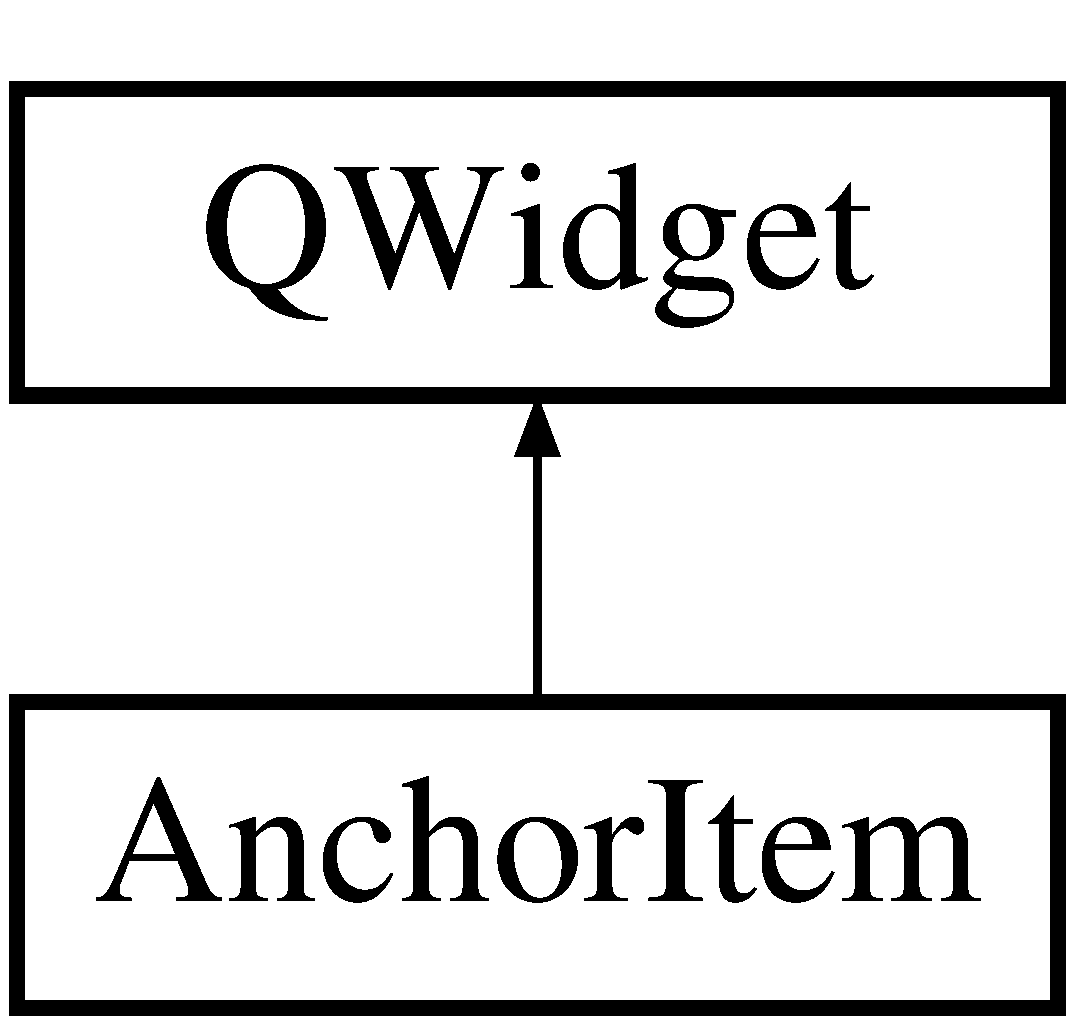
\includegraphics[height=2.000000cm]{classAnchorItem}
\end{center}
\end{figure}
\subsection*{Public Member Functions}
\begin{DoxyCompactItemize}
\item 
\hyperlink{classAnchorItem_a06c620842bbbe71cd1066f08a5000196}{Anchor\+Item} (Item\+Type type, int64\+\_\+t timestamp, unsigned long time\+Position, unsigned long total\+Time, unsigned long frame\+Number, unsigned long frame\+Count, Q\+Widget $\ast$parent, bool is\+Set=true, bool display\+Time=false)
\item 
\hyperlink{classAnchorItem_aa53b59e4ced3b72ed61c28d467bf822f}{$\sim$\+Anchor\+Item} ()
\item 
Item\+Type \hyperlink{classAnchorItem_a3cb5fa754bc1bfd9bad4dd6e6ff22bb6}{get\+\_\+type} ()
\item 
bool \hyperlink{classAnchorItem_aff8a1bd4b6c6645fd1cec15ce4ba8474}{is\+\_\+set} ()
\item 
void \hyperlink{classAnchorItem_ae900d01f71ff480d4bbbfee8ef7fac80}{set\+\_\+highlight} (bool set)
\item 
int64\+\_\+t \hyperlink{classAnchorItem_a3bdcec9b92921e16810b5251a5273afa}{get\+\_\+timestamp} () const 
\item 
void \hyperlink{classAnchorItem_a3905061f30d8b6a77b00ad52311605af}{display\+\_\+time} ()
\item 
void \hyperlink{classAnchorItem_a4b9fb672e2ebc5289c116027dc8a383d}{display\+\_\+frame\+\_\+num} ()
\end{DoxyCompactItemize}
\subsection*{Protected Member Functions}
\begin{DoxyCompactItemize}
\item 
bool \hyperlink{classAnchorItem_a78686f7c51def036159b1dfe56be9b33}{event\+Filter} (Q\+Object $\ast$object, Q\+Event $\ast$event)
\end{DoxyCompactItemize}


\subsection{Detailed Description}


Definition at line 20 of file anchoritem.\+h.



\subsection{Constructor \& Destructor Documentation}
\hypertarget{classAnchorItem_a06c620842bbbe71cd1066f08a5000196}{}\index{Anchor\+Item@{Anchor\+Item}!Anchor\+Item@{Anchor\+Item}}
\index{Anchor\+Item@{Anchor\+Item}!Anchor\+Item@{Anchor\+Item}}
\subsubsection[{Anchor\+Item}]{\setlength{\rightskip}{0pt plus 5cm}Anchor\+Item\+::\+Anchor\+Item (
\begin{DoxyParamCaption}
\item[{Item\+Type}]{type, }
\item[{int64\+\_\+t}]{timestamp, }
\item[{unsigned long}]{time\+Position, }
\item[{unsigned long}]{total\+Time, }
\item[{unsigned long}]{frame\+Number, }
\item[{unsigned long}]{frame\+Count, }
\item[{Q\+Widget $\ast$}]{parent, }
\item[{bool}]{is\+Set = {\ttfamily true}, }
\item[{bool}]{display\+Time = {\ttfamily false}}
\end{DoxyParamCaption}
)}\label{classAnchorItem_a06c620842bbbe71cd1066f08a5000196}
Constructor 
\begin{DoxyParams}{Parameters}
{\em type} & Item type \\
\hline
{\em timestamp} & Timestamp \\
\hline
{\em time\+Position} & Time position \\
\hline
{\em total\+Time} & Total video time \\
\hline
{\em frame\+Number} & Fram number \\
\hline
{\em frame\+Count} & Number of frames in the video \\
\hline
{\em parent} & Parent widget \\
\hline
{\em is\+Set} & Is the item set? Works only with E\+N\+D Item\+Type \\
\hline
{\em display\+Time} & True -\/ display time. False -\/ display frame number \\
\hline
\end{DoxyParams}


Definition at line 12 of file anchoritem.\+cpp.

\hypertarget{classAnchorItem_aa53b59e4ced3b72ed61c28d467bf822f}{}\index{Anchor\+Item@{Anchor\+Item}!````~Anchor\+Item@{$\sim$\+Anchor\+Item}}
\index{````~Anchor\+Item@{$\sim$\+Anchor\+Item}!Anchor\+Item@{Anchor\+Item}}
\subsubsection[{$\sim$\+Anchor\+Item}]{\setlength{\rightskip}{0pt plus 5cm}Anchor\+Item\+::$\sim$\+Anchor\+Item (
\begin{DoxyParamCaption}
{}
\end{DoxyParamCaption}
)}\label{classAnchorItem_aa53b59e4ced3b72ed61c28d467bf822f}
Destructor 

Definition at line 103 of file anchoritem.\+cpp.



\subsection{Member Function Documentation}
\hypertarget{classAnchorItem_a4b9fb672e2ebc5289c116027dc8a383d}{}\index{Anchor\+Item@{Anchor\+Item}!display\+\_\+frame\+\_\+num@{display\+\_\+frame\+\_\+num}}
\index{display\+\_\+frame\+\_\+num@{display\+\_\+frame\+\_\+num}!Anchor\+Item@{Anchor\+Item}}
\subsubsection[{display\+\_\+frame\+\_\+num}]{\setlength{\rightskip}{0pt plus 5cm}void Anchor\+Item\+::display\+\_\+frame\+\_\+num (
\begin{DoxyParamCaption}
{}
\end{DoxyParamCaption}
)}\label{classAnchorItem_a4b9fb672e2ebc5289c116027dc8a383d}
Displays values as frame numbers. 

Definition at line 148 of file anchoritem.\+cpp.

\hypertarget{classAnchorItem_a3905061f30d8b6a77b00ad52311605af}{}\index{Anchor\+Item@{Anchor\+Item}!display\+\_\+time@{display\+\_\+time}}
\index{display\+\_\+time@{display\+\_\+time}!Anchor\+Item@{Anchor\+Item}}
\subsubsection[{display\+\_\+time}]{\setlength{\rightskip}{0pt plus 5cm}void Anchor\+Item\+::display\+\_\+time (
\begin{DoxyParamCaption}
{}
\end{DoxyParamCaption}
)}\label{classAnchorItem_a3905061f30d8b6a77b00ad52311605af}
Displays values as time positions. 

Definition at line 138 of file anchoritem.\+cpp.

\hypertarget{classAnchorItem_a78686f7c51def036159b1dfe56be9b33}{}\index{Anchor\+Item@{Anchor\+Item}!event\+Filter@{event\+Filter}}
\index{event\+Filter@{event\+Filter}!Anchor\+Item@{Anchor\+Item}}
\subsubsection[{event\+Filter}]{\setlength{\rightskip}{0pt plus 5cm}bool Anchor\+Item\+::event\+Filter (
\begin{DoxyParamCaption}
\item[{Q\+Object $\ast$}]{object, }
\item[{Q\+Event $\ast$}]{event}
\end{DoxyParamCaption}
)\hspace{0.3cm}{\ttfamily [protected]}}\label{classAnchorItem_a78686f7c51def036159b1dfe56be9b33}
Filters Enter and Leave events for item highlighting when hovering 
\begin{DoxyParams}{Parameters}
{\em object} & Object of the event \\
\hline
{\em event} & Event \\
\hline
\end{DoxyParams}
\begin{DoxyReturn}{Returns}
False -\/ propagate event further. True -\/ do not propagate. 
\end{DoxyReturn}


Definition at line 75 of file anchoritem.\+cpp.

\hypertarget{classAnchorItem_a3bdcec9b92921e16810b5251a5273afa}{}\index{Anchor\+Item@{Anchor\+Item}!get\+\_\+timestamp@{get\+\_\+timestamp}}
\index{get\+\_\+timestamp@{get\+\_\+timestamp}!Anchor\+Item@{Anchor\+Item}}
\subsubsection[{get\+\_\+timestamp}]{\setlength{\rightskip}{0pt plus 5cm}int64\+\_\+t Anchor\+Item\+::get\+\_\+timestamp (
\begin{DoxyParamCaption}
{}
\end{DoxyParamCaption}
) const}\label{classAnchorItem_a3bdcec9b92921e16810b5251a5273afa}
Returns timestamp. \begin{DoxyReturn}{Returns}
timestamp
\end{DoxyReturn}
void \hyperlink{classAnchorItem_ae900d01f71ff480d4bbbfee8ef7fac80}{Anchor\+Item\+::set\+\_\+highlight(bool set)} \{ if (set) set\+Style\+Sheet(background\+Color\+Active); else set\+Style\+Sheet(background\+Color\+Inactive);

\begin{DoxyVerb}QFont nameFont = name->font();
nameFont.setUnderline(set);
name->setFont(nameFont);
\end{DoxyVerb}
 \} 

Definition at line 133 of file anchoritem.\+cpp.

\hypertarget{classAnchorItem_a3cb5fa754bc1bfd9bad4dd6e6ff22bb6}{}\index{Anchor\+Item@{Anchor\+Item}!get\+\_\+type@{get\+\_\+type}}
\index{get\+\_\+type@{get\+\_\+type}!Anchor\+Item@{Anchor\+Item}}
\subsubsection[{get\+\_\+type}]{\setlength{\rightskip}{0pt plus 5cm}Item\+Type Anchor\+Item\+::get\+\_\+type (
\begin{DoxyParamCaption}
{}
\end{DoxyParamCaption}
)}\label{classAnchorItem_a3cb5fa754bc1bfd9bad4dd6e6ff22bb6}
Returns type of this item. \begin{DoxyReturn}{Returns}
Item type 
\end{DoxyReturn}


Definition at line 108 of file anchoritem.\+cpp.

\hypertarget{classAnchorItem_aff8a1bd4b6c6645fd1cec15ce4ba8474}{}\index{Anchor\+Item@{Anchor\+Item}!is\+\_\+set@{is\+\_\+set}}
\index{is\+\_\+set@{is\+\_\+set}!Anchor\+Item@{Anchor\+Item}}
\subsubsection[{is\+\_\+set}]{\setlength{\rightskip}{0pt plus 5cm}bool Anchor\+Item\+::is\+\_\+set (
\begin{DoxyParamCaption}
{}
\end{DoxyParamCaption}
)}\label{classAnchorItem_aff8a1bd4b6c6645fd1cec15ce4ba8474}
Is the object set? is\+Set works only with E\+N\+D Item\+Type. \begin{DoxyReturn}{Returns}
is\+Set. 
\end{DoxyReturn}


Definition at line 113 of file anchoritem.\+cpp.

\hypertarget{classAnchorItem_ae900d01f71ff480d4bbbfee8ef7fac80}{}\index{Anchor\+Item@{Anchor\+Item}!set\+\_\+highlight@{set\+\_\+highlight}}
\index{set\+\_\+highlight@{set\+\_\+highlight}!Anchor\+Item@{Anchor\+Item}}
\subsubsection[{set\+\_\+highlight}]{\setlength{\rightskip}{0pt plus 5cm}void Anchor\+Item\+::set\+\_\+highlight (
\begin{DoxyParamCaption}
\item[{bool}]{set}
\end{DoxyParamCaption}
)}\label{classAnchorItem_ae900d01f71ff480d4bbbfee8ef7fac80}
Sets highlighting. Works with \hyperlink{classAnchorItem_a78686f7c51def036159b1dfe56be9b33}{event\+Filter()}. 
\begin{DoxyParams}{Parameters}
{\em set} & True -\/ highlight always on. False -\/ highlight set according item hover. \\
\hline
\end{DoxyParams}


Definition at line 93 of file anchoritem.\+cpp.



The documentation for this class was generated from the following files\+:\begin{DoxyCompactItemize}
\item 
headers/\hyperlink{anchoritem_8h}{anchoritem.\+h}\item 
sources/\hyperlink{anchoritem_8cpp}{anchoritem.\+cpp}\end{DoxyCompactItemize}

\hypertarget{classAVWriter}{}\section{A\+V\+Writer Class Reference}
\label{classAVWriter}\index{A\+V\+Writer@{A\+V\+Writer}}
\subsection*{Public Member Functions}
\begin{DoxyCompactItemize}
\item 
bool \hyperlink{classAVWriter_a07d7498d6d2dda57dd1d61432f09067c}{initialize\+\_\+output} (std\+::string filename, A\+V\+Stream const $\ast$in\+Video\+Stream, A\+V\+Stream const $\ast$in\+Audio\+Stream, char const $\ast$in\+Format\+Name, std\+::string in\+File\+Extension)
\item 
bool \hyperlink{classAVWriter_a6a7f5e05adb1e6c62baf2012a2cfc7cc}{close\+\_\+output} ()
\item 
bool \hyperlink{classAVWriter_af2d42cafca32a4d9fe45dab2e3ae9716}{write\+\_\+video\+\_\+frame} (\hyperlink{classVideoFrame}{Video\+Frame} \&frame)
\item 
bool \hyperlink{classAVWriter_ac20a509a57e2f3dbd9a7319e267ea3e4}{write\+\_\+audio\+\_\+packet} (A\+V\+Packet \&pkt)
\item 
bool \hyperlink{classAVWriter_a1e65c6ce5f555bb7c514fafbff6f407a}{write\+\_\+last\+\_\+frames} ()
\end{DoxyCompactItemize}


\subsection{Detailed Description}


Definition at line 30 of file avwriter.\+h.



\subsection{Member Function Documentation}
\hypertarget{classAVWriter_a6a7f5e05adb1e6c62baf2012a2cfc7cc}{}\index{A\+V\+Writer@{A\+V\+Writer}!close\+\_\+output@{close\+\_\+output}}
\index{close\+\_\+output@{close\+\_\+output}!A\+V\+Writer@{A\+V\+Writer}}
\subsubsection[{close\+\_\+output}]{\setlength{\rightskip}{0pt plus 5cm}bool A\+V\+Writer\+::close\+\_\+output (
\begin{DoxyParamCaption}
{}
\end{DoxyParamCaption}
)}\label{classAVWriter_a6a7f5e05adb1e6c62baf2012a2cfc7cc}
Correct closing of the output file. \begin{DoxyReturn}{Returns}
True if successful 
\end{DoxyReturn}


Definition at line 185 of file avwriter.\+cpp.

\hypertarget{classAVWriter_a07d7498d6d2dda57dd1d61432f09067c}{}\index{A\+V\+Writer@{A\+V\+Writer}!initialize\+\_\+output@{initialize\+\_\+output}}
\index{initialize\+\_\+output@{initialize\+\_\+output}!A\+V\+Writer@{A\+V\+Writer}}
\subsubsection[{initialize\+\_\+output}]{\setlength{\rightskip}{0pt plus 5cm}bool A\+V\+Writer\+::initialize\+\_\+output (
\begin{DoxyParamCaption}
\item[{std\+::string}]{filename, }
\item[{A\+V\+Stream const $\ast$}]{in\+Video\+Stream, }
\item[{A\+V\+Stream const $\ast$}]{in\+Audio\+Stream, }
\item[{char const $\ast$}]{in\+Format\+Name, }
\item[{std\+::string}]{in\+File\+Extension}
\end{DoxyParamCaption}
)}\label{classAVWriter_a07d7498d6d2dda57dd1d61432f09067c}
Initializes contexts, opens codecs and opens the output file for writing. 
\begin{DoxyParams}{Parameters}
{\em filename} & Output filename \\
\hline
{\em in\+Video\+Stream} & Input video stream \\
\hline
{\em in\+Audio\+Stream} & Input audio stream \\
\hline
{\em in\+Format\+Name} & Name of the input file format \\
\hline
{\em in\+File\+Extension} & Extension of the input file \\
\hline
\end{DoxyParams}
\begin{DoxyReturn}{Returns}
True if initialization successful 
\end{DoxyReturn}
choose extension according the file format\+: std\+::string str(format\+Context-\/$>$iformat-\/$>$name); std\+::string ext = str.\+substr(0, str.\+find(\textquotesingle{},\textquotesingle{})); filename += \char`\"{}.\char`\"{}; filename += ext; q\+Debug() $<$$<$ ext.\+c\+\_\+str(); avformat\+\_\+alloc\+\_\+output\+\_\+context2(\&format\+Context2, N\+U\+L\+L, ext.\+c\+\_\+str(), N\+U\+L\+L); // allocation of output context

\begin{DoxyVerb} Output video format deduction form the (output) filename.
 It is disabled because format should match the input format so as extra settings is not needed.
 Encoding to some other formats might not be valid especially because mixed PTS and DTS
\end{DoxyVerb}


std\+::string original\+Filename = filename; // \char`\"{}filename\char`\"{} might change the extension if needed; \char`\"{}original\+Filename\char`\"{} stores the argument Allocating output media context avformat\+\_\+alloc\+\_\+output\+\_\+context2(\&format\+Context, nullptr, nullptr, filename.\+c\+\_\+str()); // allocation of output context

if (!format\+Context $\vert$$\vert$ format\+Context-\/$>$oformat-\/$>$video\+\_\+codec == A\+V\+\_\+\+C\+O\+D\+E\+C\+\_\+\+I\+D\+\_\+\+N\+O\+N\+E) \{ if (!format\+Context) \{ q\+Debug() $<$$<$ \char`\"{}\+Warning\+: Could not deduce output format from file extension. Deducing from input format instead.\char`\"{}; \} else \{ q\+Debug() $<$$<$ \char`\"{}\+Warning\+: File format deduced from file extension does not support video. Deducing from input format instead.\char`\"{}; avformat\+\_\+free\+\_\+context(format\+Context); format\+Context = nullptr; \}

Try allocate format\+Context according to input format name and set appropriate extension The new extension is added after the previous one (user might want to have a dot in the filename) std\+::string str(in\+Format\+Name); std\+::string ext = str.\+substr(0, str.\+find(\textquotesingle{},\textquotesingle{})); // Finds first extension that belongs to given file format if (!ext.empty()) // Appropriate extension found \{ filename = original\+Filename + \char`\"{}.\char`\"{} + ext; q\+Debug() $<$$<$ ext.\+c\+\_\+str(); avformat\+\_\+alloc\+\_\+output\+\_\+context2(\&format\+Context, N\+U\+L\+L, ext.\+c\+\_\+str(), N\+U\+L\+L); // allocation of output context \} \}

Definition at line 32 of file avwriter.\+cpp.

\hypertarget{classAVWriter_ac20a509a57e2f3dbd9a7319e267ea3e4}{}\index{A\+V\+Writer@{A\+V\+Writer}!write\+\_\+audio\+\_\+packet@{write\+\_\+audio\+\_\+packet}}
\index{write\+\_\+audio\+\_\+packet@{write\+\_\+audio\+\_\+packet}!A\+V\+Writer@{A\+V\+Writer}}
\subsubsection[{write\+\_\+audio\+\_\+packet}]{\setlength{\rightskip}{0pt plus 5cm}bool A\+V\+Writer\+::write\+\_\+audio\+\_\+packet (
\begin{DoxyParamCaption}
\item[{A\+V\+Packet \&}]{pkt}
\end{DoxyParamCaption}
)}\label{classAVWriter_ac20a509a57e2f3dbd9a7319e267ea3e4}
Writes the audio packet to the output audio stream. 
\begin{DoxyParams}{Parameters}
{\em pkt} & Packet to be written \\
\hline
\end{DoxyParams}
\begin{DoxyReturn}{Returns}
True if successful 
\end{DoxyReturn}


Definition at line 416 of file avwriter.\+cpp.

\hypertarget{classAVWriter_a1e65c6ce5f555bb7c514fafbff6f407a}{}\index{A\+V\+Writer@{A\+V\+Writer}!write\+\_\+last\+\_\+frames@{write\+\_\+last\+\_\+frames}}
\index{write\+\_\+last\+\_\+frames@{write\+\_\+last\+\_\+frames}!A\+V\+Writer@{A\+V\+Writer}}
\subsubsection[{write\+\_\+last\+\_\+frames}]{\setlength{\rightskip}{0pt plus 5cm}bool A\+V\+Writer\+::write\+\_\+last\+\_\+frames (
\begin{DoxyParamCaption}
{}
\end{DoxyParamCaption}
)}\label{classAVWriter_a1e65c6ce5f555bb7c514fafbff6f407a}
Writes all frames remaining in the encoder; emptying buffers. \begin{DoxyReturn}{Returns}
True if successful 
\end{DoxyReturn}


Definition at line 376 of file avwriter.\+cpp.

\hypertarget{classAVWriter_af2d42cafca32a4d9fe45dab2e3ae9716}{}\index{A\+V\+Writer@{A\+V\+Writer}!write\+\_\+video\+\_\+frame@{write\+\_\+video\+\_\+frame}}
\index{write\+\_\+video\+\_\+frame@{write\+\_\+video\+\_\+frame}!A\+V\+Writer@{A\+V\+Writer}}
\subsubsection[{write\+\_\+video\+\_\+frame}]{\setlength{\rightskip}{0pt plus 5cm}bool A\+V\+Writer\+::write\+\_\+video\+\_\+frame (
\begin{DoxyParamCaption}
\item[{{\bf Video\+Frame} \&}]{frame}
\end{DoxyParamCaption}
)}\label{classAVWriter_af2d42cafca32a4d9fe45dab2e3ae9716}
Writes the video frame to the output video stream. 
\begin{DoxyParams}{Parameters}
{\em frame} & Frame to be written \\
\hline
\end{DoxyParams}
\begin{DoxyReturn}{Returns}
True if successful 
\end{DoxyReturn}
Commented because not tested if (format\+Context-\/$>$oformat-\/$>$flags \& A\+V\+F\+M\+T\+\_\+\+R\+A\+W\+P\+I\+C\+T\+U\+R\+E) \{ // avoiding data copy with some raw video muxers q\+Debug() $<$$<$ \char`\"{}raw\char`\"{}; pkt.\+flags $\vert$= A\+V\+\_\+\+P\+K\+T\+\_\+\+F\+L\+A\+G\+\_\+\+K\+E\+Y; pkt.\+stream\+\_\+index = video\+Stream-\/$>$index; pkt.\+data = (uint8\+\_\+t $\ast$)av\+Frame; pkt.\+size = sizeof(\+A\+V\+Picture); pkt.\+pts = pkt.\+dts = frame.\+get\+\_\+timestamp(); \} else \{

\} 

Definition at line 309 of file avwriter.\+cpp.



The documentation for this class was generated from the following files\+:\begin{DoxyCompactItemize}
\item 
headers/\hyperlink{avwriter_8h}{avwriter.\+h}\item 
sources/\hyperlink{avwriter_8cpp}{avwriter.\+cpp}\end{DoxyCompactItemize}

\hypertarget{structCharacteristics}{}\section{Characteristics Struct Reference}
\label{structCharacteristics}\index{Characteristics@{Characteristics}}
\subsection*{Public Member Functions}
\begin{DoxyCompactItemize}
\item 
\hypertarget{structCharacteristics_a9a27d2d685207d583d90715ed1dfa4dc}{}{\footnotesize template$<$class Archive $>$ }\\void {\bfseries serialize} (Archive \&archive)\label{structCharacteristics_a9a27d2d685207d583d90715ed1dfa4dc}

\item 
\hypertarget{structCharacteristics_aa36f20424280a476153311b495ab952c}{}{\bfseries Characteristics} (unsigned int shape, bool defocus, unsigned int defocus\+Size, bool draw\+Inside, \hyperlink{structObjectColor}{Object\+Color} color, unsigned int color\+I\+D, bool draw\+Border, \hyperlink{structObjectColor}{Object\+Color} border\+Color, unsigned int border\+Color\+I\+D, int border\+Thickness)\label{structCharacteristics_aa36f20424280a476153311b495ab952c}

\end{DoxyCompactItemize}
\subsection*{Public Attributes}
\begin{DoxyCompactItemize}
\item 
\hypertarget{structCharacteristics_a5bbaeeb14e3a875db08ecea39ffcea54}{}unsigned int {\bfseries shape}\label{structCharacteristics_a5bbaeeb14e3a875db08ecea39ffcea54}

\item 
\hypertarget{structCharacteristics_a48faeb5b1352a5813fc99d29fe30a1f2}{}bool {\bfseries defocus}\label{structCharacteristics_a48faeb5b1352a5813fc99d29fe30a1f2}

\item 
\hypertarget{structCharacteristics_a7d761e46119e285da0bd826a4a6774ec}{}unsigned int {\bfseries defocus\+Size}\label{structCharacteristics_a7d761e46119e285da0bd826a4a6774ec}

\item 
\hypertarget{structCharacteristics_aad446cd74d72f5e734e70583acf261bd}{}bool {\bfseries draw\+Inside}\label{structCharacteristics_aad446cd74d72f5e734e70583acf261bd}

\item 
\hypertarget{structCharacteristics_a8f408d8583789749a2c9b4b55715303d}{}\hyperlink{structObjectColor}{Object\+Color} {\bfseries color}\label{structCharacteristics_a8f408d8583789749a2c9b4b55715303d}

\item 
\hypertarget{structCharacteristics_adef6271d166c73d67319450e2fc42d0e}{}unsigned int {\bfseries color\+I\+D}\label{structCharacteristics_adef6271d166c73d67319450e2fc42d0e}

\item 
\hypertarget{structCharacteristics_a02be9b757d42c816373e10e1ee6fa2dc}{}bool {\bfseries draw\+Border}\label{structCharacteristics_a02be9b757d42c816373e10e1ee6fa2dc}

\item 
\hypertarget{structCharacteristics_a4a3d1795f5ed670e4ac4fee1298efc33}{}\hyperlink{structObjectColor}{Object\+Color} {\bfseries border\+Color}\label{structCharacteristics_a4a3d1795f5ed670e4ac4fee1298efc33}

\item 
\hypertarget{structCharacteristics_a92d29fbdb8e4a4662723084fd18b1ee4}{}unsigned int {\bfseries border\+Color\+I\+D}\label{structCharacteristics_a92d29fbdb8e4a4662723084fd18b1ee4}

\item 
\hypertarget{structCharacteristics_a5c903831d39edbec3a3d1509b4070444}{}int {\bfseries border\+Thickness}\label{structCharacteristics_a5c903831d39edbec3a3d1509b4070444}

\end{DoxyCompactItemize}


\subsection{Detailed Description}


Definition at line 56 of file selection.\+h.



The documentation for this struct was generated from the following file\+:\begin{DoxyCompactItemize}
\item 
headers/\hyperlink{selection_8h}{selection.\+h}\end{DoxyCompactItemize}

\hypertarget{classColors}{}\section{Colors Class Reference}
\label{classColors}\index{Colors@{Colors}}
\subsection*{Static Public Attributes}
\begin{DoxyCompactItemize}
\item 
\hypertarget{classColors_a01cf6a665fe0e66e5462ace37acd428d}{}static const unsigned {\bfseries B\+L\+A\+C\+K} = 1\label{classColors_a01cf6a665fe0e66e5462ace37acd428d}

\item 
\hypertarget{classColors_a1d66700618d1bad0cb6286120747110d}{}static const unsigned {\bfseries G\+R\+A\+Y} = 2\label{classColors_a1d66700618d1bad0cb6286120747110d}

\item 
\hypertarget{classColors_a34001465db0310d6061378785fe6b77f}{}static const unsigned {\bfseries S\+I\+L\+V\+E\+R} = 3\label{classColors_a34001465db0310d6061378785fe6b77f}

\item 
\hypertarget{classColors_a88c3d5ac0c91ea16f14b4a4631619cf0}{}static const unsigned {\bfseries W\+H\+I\+T\+E} = 4\label{classColors_a88c3d5ac0c91ea16f14b4a4631619cf0}

\item 
\hypertarget{classColors_a046700ffb5fe8310004d7cdd3aa3f14c}{}static const unsigned {\bfseries R\+E\+D} = 5\label{classColors_a046700ffb5fe8310004d7cdd3aa3f14c}

\item 
\hypertarget{classColors_a87a37b010fb2b2203a29a285f793bcc4}{}static const unsigned {\bfseries G\+R\+E\+E\+N} = 6\label{classColors_a87a37b010fb2b2203a29a285f793bcc4}

\item 
\hypertarget{classColors_ae5bd79999a8ea041d2fd26abcda78ca5}{}static const unsigned {\bfseries B\+L\+U\+E} = 7\label{classColors_ae5bd79999a8ea041d2fd26abcda78ca5}

\item 
\hypertarget{classColors_ab706eb62c9c721aed157d5802717d0a8}{}static const unsigned {\bfseries Y\+E\+L\+L\+O\+W} = 8\label{classColors_ab706eb62c9c721aed157d5802717d0a8}

\item 
\hypertarget{classColors_a8e7cbfe9ab77bf753374e9039a55b3f9}{}static const unsigned {\bfseries C\+Y\+A\+N} = 9\label{classColors_a8e7cbfe9ab77bf753374e9039a55b3f9}

\item 
\hypertarget{classColors_a770dc1c7f2e675277c0eca596eb02d10}{}static const unsigned {\bfseries M\+A\+G\+E\+N\+T\+A} = 10\label{classColors_a770dc1c7f2e675277c0eca596eb02d10}

\end{DoxyCompactItemize}


\subsection{Detailed Description}


Definition at line 10 of file colors.\+h.



The documentation for this class was generated from the following files\+:\begin{DoxyCompactItemize}
\item 
headers/\hyperlink{colors_8h}{colors.\+h}\item 
sources/\hyperlink{colors_8cpp}{colors.\+cpp}\end{DoxyCompactItemize}

\hypertarget{classFFmpegPlayer}{}\section{F\+Fmpeg\+Player Class Reference}
\label{classFFmpegPlayer}\index{F\+Fmpeg\+Player@{F\+Fmpeg\+Player}}
\subsection*{Public Member Functions}
\begin{DoxyCompactItemize}
\item 
\hyperlink{classFFmpegPlayer_ab51ec3c9c3d40680a69b02bda9767341}{F\+Fmpeg\+Player} (std\+::string video\+Addr, Q\+Progress\+Dialog const $\ast$progress\+Dialog)
\item 
\hyperlink{classFFmpegPlayer_ab6aa2a58362cee1c23d90bfa84164205}{$\sim$\+F\+Fmpeg\+Player} ()
\item 
double \hyperlink{classFFmpegPlayer_a2cdc53e1813de0723f2bfe869f0ad504}{get\+\_\+fps} () const 
\item 
unsigned long \hyperlink{classFFmpegPlayer_afb2c1a93fd9cc360340ff989b41500bd}{get\+\_\+frame\+\_\+count} () const 
\item 
unsigned long \hyperlink{classFFmpegPlayer_a2f71f53316479782cb09f78f1383380b}{get\+\_\+total\+\_\+time} () const 
\item 
unsigned int \hyperlink{classFFmpegPlayer_acfbe5305c4e30623ecc791519e2625d0}{get\+\_\+height} () const 
\item 
unsigned int \hyperlink{classFFmpegPlayer_a52cc701b9fdf9882a65be3f979f8d5a7}{get\+\_\+width} () const 
\item 
A\+V\+Stream const $\ast$ \hyperlink{classFFmpegPlayer_a5ed6acba145aeb2a63626f6008b2b56e}{get\+\_\+video\+\_\+stream} ()
\item 
A\+V\+Stream const $\ast$ \hyperlink{classFFmpegPlayer_a134ebdd27b8edf065fcd3e825ec5e114}{get\+\_\+audio\+\_\+stream} ()
\item 
bool \hyperlink{classFFmpegPlayer_a7f14f3411a6f959f3e796d713de1b056}{get\+\_\+frame\+\_\+by\+\_\+time} (\hyperlink{classVideoFrame}{Video\+Frame} $\ast$result\+Frame, unsigned long time)
\item 
bool \hyperlink{classFFmpegPlayer_a4561d19e9d7b0820c202037d754bb049}{get\+\_\+frame\+\_\+by\+\_\+timestamp} (\hyperlink{classVideoFrame}{Video\+Frame} $\ast$result\+Frame, int64\+\_\+t timestamp)
\item 
bool \hyperlink{classFFmpegPlayer_a7ba674baeb349fd6cba4514993abd745}{get\+\_\+frame\+\_\+by\+\_\+number} (\hyperlink{classVideoFrame}{Video\+Frame} $\ast$result\+Frame, unsigned long frame\+Number)
\item 
bool \hyperlink{classFFmpegPlayer_a448e643bcbb4583bdad3ba9b5f615ee4}{get\+\_\+next\+\_\+frame} (\hyperlink{classVideoFrame}{Video\+Frame} $\ast$result\+Frame)
\item 
bool \hyperlink{classFFmpegPlayer_a9bf7b16453ba472819723f1f1c8a80bd}{get\+\_\+previous\+\_\+frame} (\hyperlink{classVideoFrame}{Video\+Frame} $\ast$result\+Frame)
\item 
bool \hyperlink{classFFmpegPlayer_a5218c55d82306ac58df1667579878f74}{read\+\_\+frame} (A\+V\+Packet \&packet, bool only\+Video\+Packets=true, bool $\ast$is\+Audio=nullptr)
\item 
bool \hyperlink{classFFmpegPlayer_a4c70bf1467385856982f391158de3e49}{get\+\_\+current\+\_\+frame} (\hyperlink{classVideoFrame}{Video\+Frame} $\ast$frame)
\item 
bool \hyperlink{classFFmpegPlayer_a03a7bcc6b81e74ad9d40346c8d267422}{seek\+\_\+first\+\_\+packet} ()
\item 
const char $\ast$ \hyperlink{classFFmpegPlayer_a8dc7287f8ab038a1d1e78de2b6345ece}{get\+\_\+format\+\_\+name} ()
\end{DoxyCompactItemize}


\subsection{Detailed Description}


Definition at line 42 of file ffmpegplayer.\+h.



\subsection{Constructor \& Destructor Documentation}
\hypertarget{classFFmpegPlayer_ab51ec3c9c3d40680a69b02bda9767341}{}\index{F\+Fmpeg\+Player@{F\+Fmpeg\+Player}!F\+Fmpeg\+Player@{F\+Fmpeg\+Player}}
\index{F\+Fmpeg\+Player@{F\+Fmpeg\+Player}!F\+Fmpeg\+Player@{F\+Fmpeg\+Player}}
\subsubsection[{F\+Fmpeg\+Player}]{\setlength{\rightskip}{0pt plus 5cm}F\+Fmpeg\+Player\+::\+F\+Fmpeg\+Player (
\begin{DoxyParamCaption}
\item[{std\+::string}]{video\+Addr, }
\item[{Q\+Progress\+Dialog const $\ast$}]{progress\+Dialog}
\end{DoxyParamCaption}
)}\label{classFFmpegPlayer_ab51ec3c9c3d40680a69b02bda9767341}
Constructor 
\begin{DoxyParams}{Parameters}
{\em video\+Addr} & Path to a video file \\
\hline
{\em progress\+Dialog} & Q\+T progress dialog for displaying information about video opening \\
\hline
\end{DoxyParams}


Definition at line 16 of file ffmpegplayer.\+cpp.

\hypertarget{classFFmpegPlayer_ab6aa2a58362cee1c23d90bfa84164205}{}\index{F\+Fmpeg\+Player@{F\+Fmpeg\+Player}!````~F\+Fmpeg\+Player@{$\sim$\+F\+Fmpeg\+Player}}
\index{````~F\+Fmpeg\+Player@{$\sim$\+F\+Fmpeg\+Player}!F\+Fmpeg\+Player@{F\+Fmpeg\+Player}}
\subsubsection[{$\sim$\+F\+Fmpeg\+Player}]{\setlength{\rightskip}{0pt plus 5cm}F\+Fmpeg\+Player\+::$\sim$\+F\+Fmpeg\+Player (
\begin{DoxyParamCaption}
{}
\end{DoxyParamCaption}
)}\label{classFFmpegPlayer_ab6aa2a58362cee1c23d90bfa84164205}
Destructor 

Definition at line 124 of file ffmpegplayer.\+cpp.



\subsection{Member Function Documentation}
\hypertarget{classFFmpegPlayer_a134ebdd27b8edf065fcd3e825ec5e114}{}\index{F\+Fmpeg\+Player@{F\+Fmpeg\+Player}!get\+\_\+audio\+\_\+stream@{get\+\_\+audio\+\_\+stream}}
\index{get\+\_\+audio\+\_\+stream@{get\+\_\+audio\+\_\+stream}!F\+Fmpeg\+Player@{F\+Fmpeg\+Player}}
\subsubsection[{get\+\_\+audio\+\_\+stream}]{\setlength{\rightskip}{0pt plus 5cm}const A\+V\+Stream $\ast$ F\+Fmpeg\+Player\+::get\+\_\+audio\+\_\+stream (
\begin{DoxyParamCaption}
{}
\end{DoxyParamCaption}
)}\label{classFFmpegPlayer_a134ebdd27b8edf065fcd3e825ec5e114}
Returns information about the input audio stream. \begin{DoxyReturn}{Returns}
Input audio stream 
\end{DoxyReturn}


Definition at line 247 of file ffmpegplayer.\+cpp.

\hypertarget{classFFmpegPlayer_a4c70bf1467385856982f391158de3e49}{}\index{F\+Fmpeg\+Player@{F\+Fmpeg\+Player}!get\+\_\+current\+\_\+frame@{get\+\_\+current\+\_\+frame}}
\index{get\+\_\+current\+\_\+frame@{get\+\_\+current\+\_\+frame}!F\+Fmpeg\+Player@{F\+Fmpeg\+Player}}
\subsubsection[{get\+\_\+current\+\_\+frame}]{\setlength{\rightskip}{0pt plus 5cm}bool F\+Fmpeg\+Player\+::get\+\_\+current\+\_\+frame (
\begin{DoxyParamCaption}
\item[{{\bf Video\+Frame} $\ast$}]{frame}
\end{DoxyParamCaption}
)}\label{classFFmpegPlayer_a4c70bf1467385856982f391158de3e49}
Returns the current frame that has already been read. 
\begin{DoxyParams}{Parameters}
{\em frame} & Read frame \\
\hline
\end{DoxyParams}
\begin{DoxyReturn}{Returns}
True if successful
\end{DoxyReturn}
unsigned long F\+Fmpeg\+Player\+::get\+\_\+time\+\_\+position() const \{ video\+Context-\/$>$ticks\+\_\+per\+\_\+frame; return av\+\_\+rescale\+\_\+q(get\+\_\+frame\+\_\+timestamp(), time\+Base, A\+V\+Rational\{1, V\+I\+D\+E\+O\+T\+R\+A\+C\+K\+I\+N\+G\+\_\+\+M\+S2\+D\+U\+R\+A\+T\+I\+O\+N\}); \} 

Definition at line 275 of file ffmpegplayer.\+cpp.

\hypertarget{classFFmpegPlayer_a8dc7287f8ab038a1d1e78de2b6345ece}{}\index{F\+Fmpeg\+Player@{F\+Fmpeg\+Player}!get\+\_\+format\+\_\+name@{get\+\_\+format\+\_\+name}}
\index{get\+\_\+format\+\_\+name@{get\+\_\+format\+\_\+name}!F\+Fmpeg\+Player@{F\+Fmpeg\+Player}}
\subsubsection[{get\+\_\+format\+\_\+name}]{\setlength{\rightskip}{0pt plus 5cm}char const $\ast$ F\+Fmpeg\+Player\+::get\+\_\+format\+\_\+name (
\begin{DoxyParamCaption}
{}
\end{DoxyParamCaption}
)}\label{classFFmpegPlayer_a8dc7287f8ab038a1d1e78de2b6345ece}
Returns the input file format name. \begin{DoxyReturn}{Returns}
File format name 
\end{DoxyReturn}


Definition at line 501 of file ffmpegplayer.\+cpp.

\hypertarget{classFFmpegPlayer_a2cdc53e1813de0723f2bfe869f0ad504}{}\index{F\+Fmpeg\+Player@{F\+Fmpeg\+Player}!get\+\_\+fps@{get\+\_\+fps}}
\index{get\+\_\+fps@{get\+\_\+fps}!F\+Fmpeg\+Player@{F\+Fmpeg\+Player}}
\subsubsection[{get\+\_\+fps}]{\setlength{\rightskip}{0pt plus 5cm}double F\+Fmpeg\+Player\+::get\+\_\+fps (
\begin{DoxyParamCaption}
{}
\end{DoxyParamCaption}
) const}\label{classFFmpegPlayer_a2cdc53e1813de0723f2bfe869f0ad504}
Returns information about frames per second. \begin{DoxyReturn}{Returns}
Frames per second 
\end{DoxyReturn}


Definition at line 207 of file ffmpegplayer.\+cpp.

\hypertarget{classFFmpegPlayer_a7ba674baeb349fd6cba4514993abd745}{}\index{F\+Fmpeg\+Player@{F\+Fmpeg\+Player}!get\+\_\+frame\+\_\+by\+\_\+number@{get\+\_\+frame\+\_\+by\+\_\+number}}
\index{get\+\_\+frame\+\_\+by\+\_\+number@{get\+\_\+frame\+\_\+by\+\_\+number}!F\+Fmpeg\+Player@{F\+Fmpeg\+Player}}
\subsubsection[{get\+\_\+frame\+\_\+by\+\_\+number}]{\setlength{\rightskip}{0pt plus 5cm}bool F\+Fmpeg\+Player\+::get\+\_\+frame\+\_\+by\+\_\+number (
\begin{DoxyParamCaption}
\item[{{\bf Video\+Frame} $\ast$}]{result\+Frame, }
\item[{unsigned long}]{frame\+Number}
\end{DoxyParamCaption}
)}\label{classFFmpegPlayer_a7ba674baeb349fd6cba4514993abd745}
Reads a frame by its number (index) and returns it. 
\begin{DoxyParams}{Parameters}
{\em result\+Frame} & Read frame \\
\hline
{\em frame\+Number} & Frame number (index) \\
\hline
\end{DoxyParams}
\begin{DoxyReturn}{Returns}
True if successful 
\end{DoxyReturn}


Definition at line 365 of file ffmpegplayer.\+cpp.

\hypertarget{classFFmpegPlayer_a7f14f3411a6f959f3e796d713de1b056}{}\index{F\+Fmpeg\+Player@{F\+Fmpeg\+Player}!get\+\_\+frame\+\_\+by\+\_\+time@{get\+\_\+frame\+\_\+by\+\_\+time}}
\index{get\+\_\+frame\+\_\+by\+\_\+time@{get\+\_\+frame\+\_\+by\+\_\+time}!F\+Fmpeg\+Player@{F\+Fmpeg\+Player}}
\subsubsection[{get\+\_\+frame\+\_\+by\+\_\+time}]{\setlength{\rightskip}{0pt plus 5cm}bool F\+Fmpeg\+Player\+::get\+\_\+frame\+\_\+by\+\_\+time (
\begin{DoxyParamCaption}
\item[{{\bf Video\+Frame} $\ast$}]{result\+Frame, }
\item[{unsigned long}]{time}
\end{DoxyParamCaption}
)}\label{classFFmpegPlayer_a7f14f3411a6f959f3e796d713de1b056}
Reads a frame by its time position and returns it. 
\begin{DoxyParams}{Parameters}
{\em result\+Frame} & Read frame \\
\hline
{\em time} & Time position \\
\hline
\end{DoxyParams}
\begin{DoxyReturn}{Returns}
True if successful 
\end{DoxyReturn}


Definition at line 296 of file ffmpegplayer.\+cpp.

\hypertarget{classFFmpegPlayer_a4561d19e9d7b0820c202037d754bb049}{}\index{F\+Fmpeg\+Player@{F\+Fmpeg\+Player}!get\+\_\+frame\+\_\+by\+\_\+timestamp@{get\+\_\+frame\+\_\+by\+\_\+timestamp}}
\index{get\+\_\+frame\+\_\+by\+\_\+timestamp@{get\+\_\+frame\+\_\+by\+\_\+timestamp}!F\+Fmpeg\+Player@{F\+Fmpeg\+Player}}
\subsubsection[{get\+\_\+frame\+\_\+by\+\_\+timestamp}]{\setlength{\rightskip}{0pt plus 5cm}bool F\+Fmpeg\+Player\+::get\+\_\+frame\+\_\+by\+\_\+timestamp (
\begin{DoxyParamCaption}
\item[{{\bf Video\+Frame} $\ast$}]{result\+Frame, }
\item[{int64\+\_\+t}]{timestamp}
\end{DoxyParamCaption}
)}\label{classFFmpegPlayer_a4561d19e9d7b0820c202037d754bb049}
Reads a frame by its timestamp and returns it. 
\begin{DoxyParams}{Parameters}
{\em result\+Frame} & Read frame \\
\hline
{\em timestamp} & Timestamp \\
\hline
\end{DoxyParams}
\begin{DoxyReturn}{Returns}
True if successful
\end{DoxyReturn}
exact\+Position -\/ if frame with the exact timestamp does not exist, return false; only\+Key\+Frames -\/ Seek only to keyframes -\/ faster; 

Definition at line 313 of file ffmpegplayer.\+cpp.

\hypertarget{classFFmpegPlayer_afb2c1a93fd9cc360340ff989b41500bd}{}\index{F\+Fmpeg\+Player@{F\+Fmpeg\+Player}!get\+\_\+frame\+\_\+count@{get\+\_\+frame\+\_\+count}}
\index{get\+\_\+frame\+\_\+count@{get\+\_\+frame\+\_\+count}!F\+Fmpeg\+Player@{F\+Fmpeg\+Player}}
\subsubsection[{get\+\_\+frame\+\_\+count}]{\setlength{\rightskip}{0pt plus 5cm}unsigned long F\+Fmpeg\+Player\+::get\+\_\+frame\+\_\+count (
\begin{DoxyParamCaption}
{}
\end{DoxyParamCaption}
) const}\label{classFFmpegPlayer_afb2c1a93fd9cc360340ff989b41500bd}
Returns information about number of frames. \begin{DoxyReturn}{Returns}
Number of frames 
\end{DoxyReturn}


Definition at line 214 of file ffmpegplayer.\+cpp.

\hypertarget{classFFmpegPlayer_acfbe5305c4e30623ecc791519e2625d0}{}\index{F\+Fmpeg\+Player@{F\+Fmpeg\+Player}!get\+\_\+height@{get\+\_\+height}}
\index{get\+\_\+height@{get\+\_\+height}!F\+Fmpeg\+Player@{F\+Fmpeg\+Player}}
\subsubsection[{get\+\_\+height}]{\setlength{\rightskip}{0pt plus 5cm}unsigned int F\+Fmpeg\+Player\+::get\+\_\+height (
\begin{DoxyParamCaption}
{}
\end{DoxyParamCaption}
) const}\label{classFFmpegPlayer_acfbe5305c4e30623ecc791519e2625d0}
Returns information about video height. \begin{DoxyReturn}{Returns}
Video height 
\end{DoxyReturn}


Definition at line 230 of file ffmpegplayer.\+cpp.

\hypertarget{classFFmpegPlayer_a448e643bcbb4583bdad3ba9b5f615ee4}{}\index{F\+Fmpeg\+Player@{F\+Fmpeg\+Player}!get\+\_\+next\+\_\+frame@{get\+\_\+next\+\_\+frame}}
\index{get\+\_\+next\+\_\+frame@{get\+\_\+next\+\_\+frame}!F\+Fmpeg\+Player@{F\+Fmpeg\+Player}}
\subsubsection[{get\+\_\+next\+\_\+frame}]{\setlength{\rightskip}{0pt plus 5cm}bool F\+Fmpeg\+Player\+::get\+\_\+next\+\_\+frame (
\begin{DoxyParamCaption}
\item[{{\bf Video\+Frame} $\ast$}]{result\+Frame}
\end{DoxyParamCaption}
)}\label{classFFmpegPlayer_a448e643bcbb4583bdad3ba9b5f615ee4}
Reads a frame following to the current one returns it. 
\begin{DoxyParams}{Parameters}
{\em result\+Frame} & Read frame \\
\hline
\end{DoxyParams}
\begin{DoxyReturn}{Returns}
True if successful 
\end{DoxyReturn}


Definition at line 373 of file ffmpegplayer.\+cpp.

\hypertarget{classFFmpegPlayer_a9bf7b16453ba472819723f1f1c8a80bd}{}\index{F\+Fmpeg\+Player@{F\+Fmpeg\+Player}!get\+\_\+previous\+\_\+frame@{get\+\_\+previous\+\_\+frame}}
\index{get\+\_\+previous\+\_\+frame@{get\+\_\+previous\+\_\+frame}!F\+Fmpeg\+Player@{F\+Fmpeg\+Player}}
\subsubsection[{get\+\_\+previous\+\_\+frame}]{\setlength{\rightskip}{0pt plus 5cm}bool F\+Fmpeg\+Player\+::get\+\_\+previous\+\_\+frame (
\begin{DoxyParamCaption}
\item[{{\bf Video\+Frame} $\ast$}]{result\+Frame}
\end{DoxyParamCaption}
)}\label{classFFmpegPlayer_a9bf7b16453ba472819723f1f1c8a80bd}
Reads a frame preceding to the current one returns it. 
\begin{DoxyParams}{Parameters}
{\em result\+Frame} & Read frame \\
\hline
\end{DoxyParams}
\begin{DoxyReturn}{Returns}
True if successful 
\end{DoxyReturn}


Definition at line 387 of file ffmpegplayer.\+cpp.

\hypertarget{classFFmpegPlayer_a2f71f53316479782cb09f78f1383380b}{}\index{F\+Fmpeg\+Player@{F\+Fmpeg\+Player}!get\+\_\+total\+\_\+time@{get\+\_\+total\+\_\+time}}
\index{get\+\_\+total\+\_\+time@{get\+\_\+total\+\_\+time}!F\+Fmpeg\+Player@{F\+Fmpeg\+Player}}
\subsubsection[{get\+\_\+total\+\_\+time}]{\setlength{\rightskip}{0pt plus 5cm}unsigned long F\+Fmpeg\+Player\+::get\+\_\+total\+\_\+time (
\begin{DoxyParamCaption}
{}
\end{DoxyParamCaption}
) const}\label{classFFmpegPlayer_a2f71f53316479782cb09f78f1383380b}
Returns information about video length. \begin{DoxyReturn}{Returns}
Video length in milliseconds 
\end{DoxyReturn}


Definition at line 222 of file ffmpegplayer.\+cpp.

\hypertarget{classFFmpegPlayer_a5ed6acba145aeb2a63626f6008b2b56e}{}\index{F\+Fmpeg\+Player@{F\+Fmpeg\+Player}!get\+\_\+video\+\_\+stream@{get\+\_\+video\+\_\+stream}}
\index{get\+\_\+video\+\_\+stream@{get\+\_\+video\+\_\+stream}!F\+Fmpeg\+Player@{F\+Fmpeg\+Player}}
\subsubsection[{get\+\_\+video\+\_\+stream}]{\setlength{\rightskip}{0pt plus 5cm}const A\+V\+Stream $\ast$ F\+Fmpeg\+Player\+::get\+\_\+video\+\_\+stream (
\begin{DoxyParamCaption}
{}
\end{DoxyParamCaption}
)}\label{classFFmpegPlayer_a5ed6acba145aeb2a63626f6008b2b56e}
Returns information about the input video stream. \begin{DoxyReturn}{Returns}
Input video stream 
\end{DoxyReturn}


Definition at line 240 of file ffmpegplayer.\+cpp.

\hypertarget{classFFmpegPlayer_a52cc701b9fdf9882a65be3f979f8d5a7}{}\index{F\+Fmpeg\+Player@{F\+Fmpeg\+Player}!get\+\_\+width@{get\+\_\+width}}
\index{get\+\_\+width@{get\+\_\+width}!F\+Fmpeg\+Player@{F\+Fmpeg\+Player}}
\subsubsection[{get\+\_\+width}]{\setlength{\rightskip}{0pt plus 5cm}unsigned int F\+Fmpeg\+Player\+::get\+\_\+width (
\begin{DoxyParamCaption}
{}
\end{DoxyParamCaption}
) const}\label{classFFmpegPlayer_a52cc701b9fdf9882a65be3f979f8d5a7}
Returns information about video width. \begin{DoxyReturn}{Returns}
Video width 
\end{DoxyReturn}


Definition at line 235 of file ffmpegplayer.\+cpp.

\hypertarget{classFFmpegPlayer_a5218c55d82306ac58df1667579878f74}{}\index{F\+Fmpeg\+Player@{F\+Fmpeg\+Player}!read\+\_\+frame@{read\+\_\+frame}}
\index{read\+\_\+frame@{read\+\_\+frame}!F\+Fmpeg\+Player@{F\+Fmpeg\+Player}}
\subsubsection[{read\+\_\+frame}]{\setlength{\rightskip}{0pt plus 5cm}bool F\+Fmpeg\+Player\+::read\+\_\+frame (
\begin{DoxyParamCaption}
\item[{A\+V\+Packet \&}]{packet, }
\item[{bool}]{only\+Video\+Packets = {\ttfamily true}, }
\item[{bool $\ast$}]{is\+Audio = {\ttfamily nullptr}}
\end{DoxyParamCaption}
)}\label{classFFmpegPlayer_a5218c55d82306ac58df1667579878f74}
Reads a new frame from the input video stream. The new frame is stored in result\+Frame. 
\begin{DoxyParams}{Parameters}
{\em packet} & Packet structure for storing the read packet; It is also used for returning audio packets \\
\hline
{\em only\+Video\+Packets} & If false -\/ audio packets are read as well as video packets. If true -\/ only video packets are read. \\
\hline
{\em is\+Audio} & Is set to true if the function returned an audio packet in A\+V\+Packet \&packet \\
\hline
\end{DoxyParams}
\begin{DoxyReturn}{Returns}
True if successful 
\end{DoxyReturn}


Definition at line 406 of file ffmpegplayer.\+cpp.

\hypertarget{classFFmpegPlayer_a03a7bcc6b81e74ad9d40346c8d267422}{}\index{F\+Fmpeg\+Player@{F\+Fmpeg\+Player}!seek\+\_\+first\+\_\+packet@{seek\+\_\+first\+\_\+packet}}
\index{seek\+\_\+first\+\_\+packet@{seek\+\_\+first\+\_\+packet}!F\+Fmpeg\+Player@{F\+Fmpeg\+Player}}
\subsubsection[{seek\+\_\+first\+\_\+packet}]{\setlength{\rightskip}{0pt plus 5cm}bool F\+Fmpeg\+Player\+::seek\+\_\+first\+\_\+packet (
\begin{DoxyParamCaption}
{}
\end{DoxyParamCaption}
)}\label{classFFmpegPlayer_a03a7bcc6b81e74ad9d40346c8d267422}
Rewinds the video to its beginning by seeking its first packet. \begin{DoxyReturn}{Returns}
True if successful 
\end{DoxyReturn}


Definition at line 483 of file ffmpegplayer.\+cpp.



The documentation for this class was generated from the following files\+:\begin{DoxyCompactItemize}
\item 
headers/\hyperlink{ffmpegplayer_8h}{ffmpegplayer.\+h}\item 
sources/\hyperlink{ffmpegplayer_8cpp}{ffmpegplayer.\+cpp}\end{DoxyCompactItemize}

\hypertarget{classHelpBrowser}{}\section{Help\+Browser Class Reference}
\label{classHelpBrowser}\index{Help\+Browser@{Help\+Browser}}
Inheritance diagram for Help\+Browser\+:\begin{figure}[H]
\begin{center}
\leavevmode
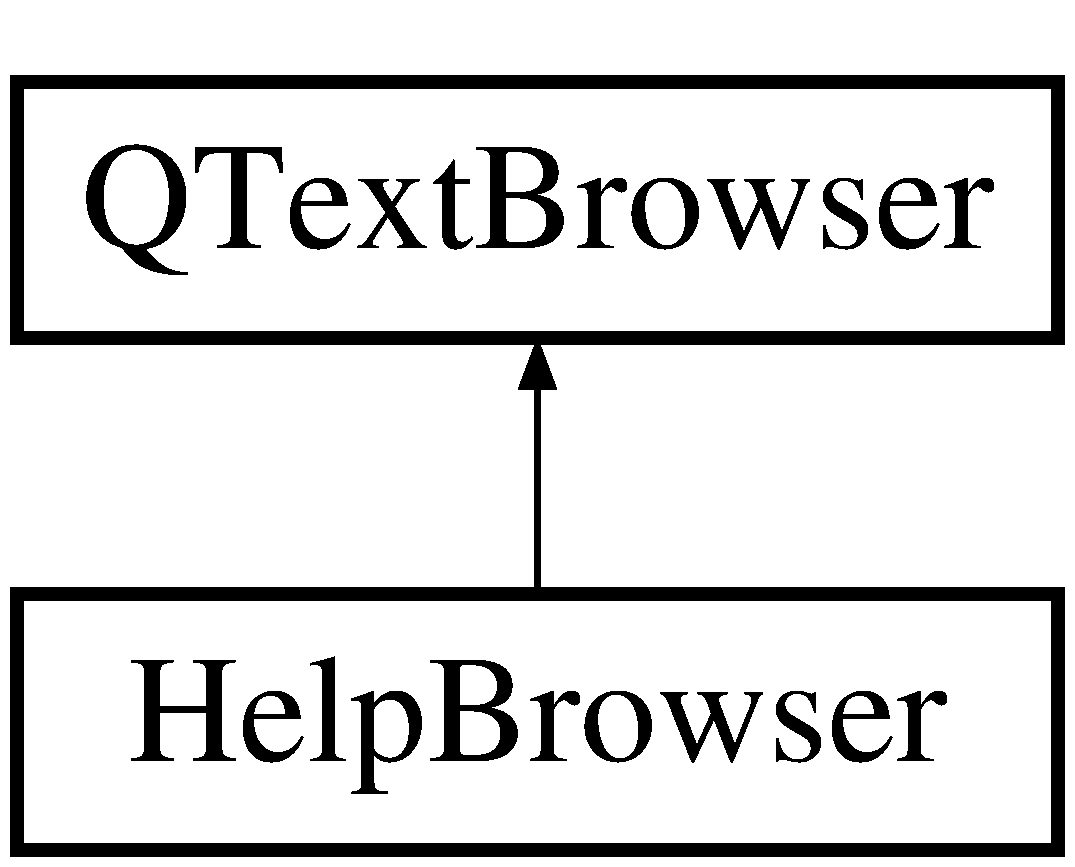
\includegraphics[height=2.000000cm]{classHelpBrowser}
\end{center}
\end{figure}
\subsection*{Public Member Functions}
\begin{DoxyCompactItemize}
\item 
\hyperlink{classHelpBrowser_a275fb39ea7346e6019c1892d5daa02cd}{Help\+Browser} (Q\+Help\+Engine $\ast$help\+Engine, Q\+Widget $\ast$parent=0)
\item 
Q\+Variant \hyperlink{classHelpBrowser_a0c87b798de23163514a604887825dbed}{load\+Resource} (int type, const Q\+Url \&name)
\end{DoxyCompactItemize}


\subsection{Detailed Description}


Definition at line 14 of file helpbrowser.\+h.



\subsection{Constructor \& Destructor Documentation}
\hypertarget{classHelpBrowser_a275fb39ea7346e6019c1892d5daa02cd}{}\index{Help\+Browser@{Help\+Browser}!Help\+Browser@{Help\+Browser}}
\index{Help\+Browser@{Help\+Browser}!Help\+Browser@{Help\+Browser}}
\subsubsection[{Help\+Browser}]{\setlength{\rightskip}{0pt plus 5cm}Help\+Browser\+::\+Help\+Browser (
\begin{DoxyParamCaption}
\item[{Q\+Help\+Engine $\ast$}]{help\+Engine, }
\item[{Q\+Widget $\ast$}]{parent = {\ttfamily 0}}
\end{DoxyParamCaption}
)}\label{classHelpBrowser_a275fb39ea7346e6019c1892d5daa02cd}
Constructor 
\begin{DoxyParams}{Parameters}
{\em help\+Engine} & Help engine with loaded help files \\
\hline
{\em parent} & Parent Widget \\
\hline
\end{DoxyParams}


Definition at line 9 of file helpbrowser.\+cpp.



\subsection{Member Function Documentation}
\hypertarget{classHelpBrowser_a0c87b798de23163514a604887825dbed}{}\index{Help\+Browser@{Help\+Browser}!load\+Resource@{load\+Resource}}
\index{load\+Resource@{load\+Resource}!Help\+Browser@{Help\+Browser}}
\subsubsection[{load\+Resource}]{\setlength{\rightskip}{0pt plus 5cm}Q\+Variant Help\+Browser\+::load\+Resource (
\begin{DoxyParamCaption}
\item[{int}]{type, }
\item[{const Q\+Url \&}]{name}
\end{DoxyParamCaption}
)}\label{classHelpBrowser_a0c87b798de23163514a604887825dbed}
Loading a resource. 
\begin{DoxyParams}{Parameters}
{\em type} & Resourse type \\
\hline
{\em name} & Resource name \\
\hline
\end{DoxyParams}
\begin{DoxyReturn}{Returns}
Found data 
\end{DoxyReturn}


Definition at line 15 of file helpbrowser.\+cpp.



The documentation for this class was generated from the following files\+:\begin{DoxyCompactItemize}
\item 
headers/\hyperlink{helpbrowser_8h}{helpbrowser.\+h}\item 
sources/\hyperlink{helpbrowser_8cpp}{helpbrowser.\+cpp}\end{DoxyCompactItemize}

\hypertarget{classImageLabel}{}\section{Image\+Label Class Reference}
\label{classImageLabel}\index{Image\+Label@{Image\+Label}}
Inheritance diagram for Image\+Label\+:\begin{figure}[H]
\begin{center}
\leavevmode
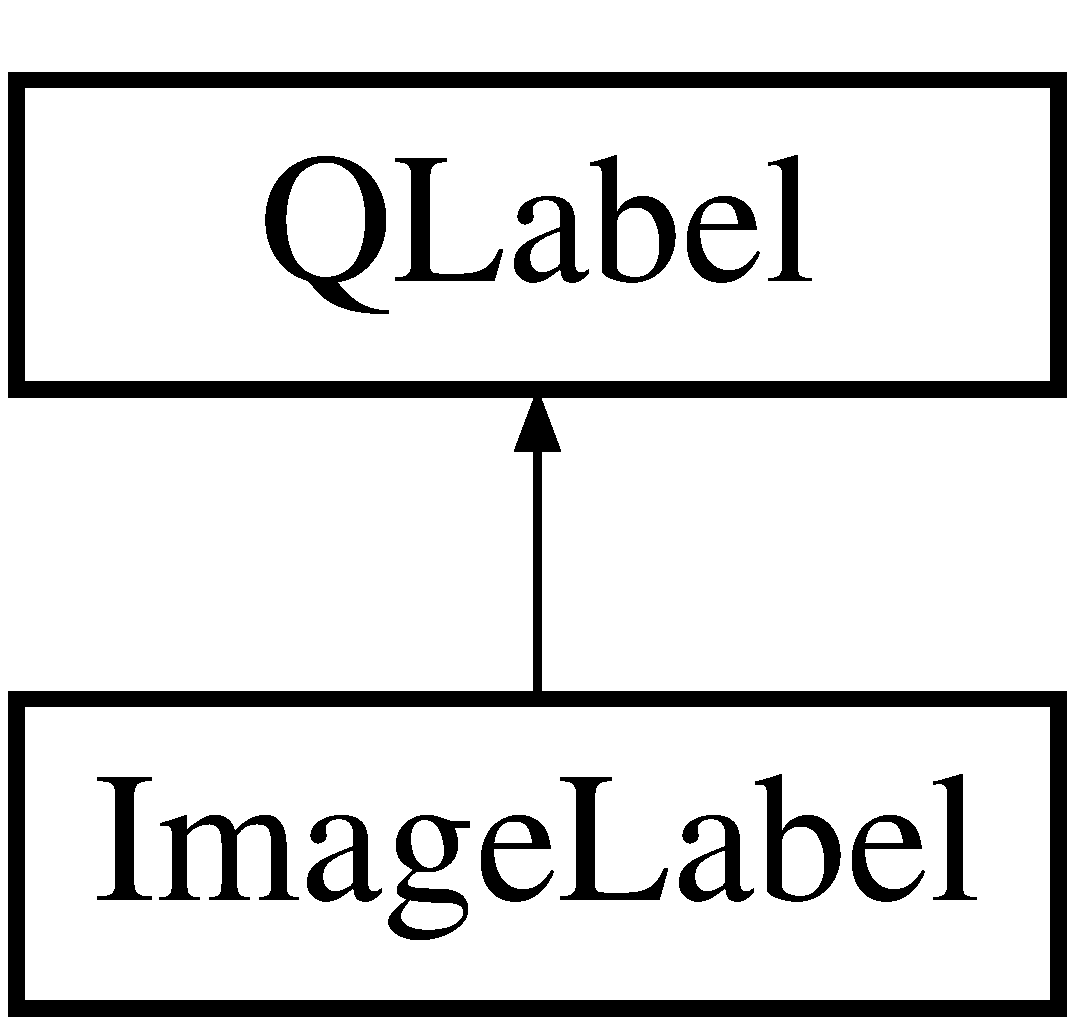
\includegraphics[height=2.000000cm]{classImageLabel}
\end{center}
\end{figure}
\subsection*{Public Member Functions}
\begin{DoxyCompactItemize}
\item 
\hyperlink{classImageLabel_a01bf7ab77bbe3d5d3f58b1cdcccc8667}{Image\+Label} (Q\+Widget $\ast$parent=0)
\item 
\hyperlink{classImageLabel_ab0caf7e09b94060541ea364e7c54d156}{$\sim$\+Image\+Label} ()
\item 
void \hyperlink{classImageLabel_acc4767a093d42e4e3eadf9a8ad70617f}{set\+\_\+image} (Q\+Image const \&image, int display\+Width, int display\+Height)
\item 
\hyperlink{structSelection}{Selection} \hyperlink{classImageLabel_ae5558dd558feade7c886a5568d24b5a3}{get\+\_\+selection} () const 
\item 
void \hyperlink{classImageLabel_a1bc29f51b2277bb51d706a95b04beb8b}{set\+\_\+selection\+\_\+enabled} (bool enabled)
\end{DoxyCompactItemize}
\subsection*{Protected Member Functions}
\begin{DoxyCompactItemize}
\item 
void \hyperlink{classImageLabel_a53568d0398cc9e07d67a5cec1da98ad1}{resize\+Event} (Q\+Resize\+Event $\ast$)
\item 
void \hyperlink{classImageLabel_a792567ff559d8e55ab22398e7ef1206d}{mouse\+Press\+Event} (Q\+Mouse\+Event $\ast$event)
\item 
void \hyperlink{classImageLabel_a50f53cf1aa569107e8acc74137afd990}{mouse\+Release\+Event} (Q\+Mouse\+Event $\ast$event)
\item 
void \hyperlink{classImageLabel_a3b57860e8b2778a46ef7700c20c55b64}{mouse\+Move\+Event} (Q\+Mouse\+Event $\ast$event)
\end{DoxyCompactItemize}


\subsection{Detailed Description}


Definition at line 16 of file imagelabel.\+h.



\subsection{Constructor \& Destructor Documentation}
\hypertarget{classImageLabel_a01bf7ab77bbe3d5d3f58b1cdcccc8667}{}\index{Image\+Label@{Image\+Label}!Image\+Label@{Image\+Label}}
\index{Image\+Label@{Image\+Label}!Image\+Label@{Image\+Label}}
\subsubsection[{Image\+Label}]{\setlength{\rightskip}{0pt plus 5cm}Image\+Label\+::\+Image\+Label (
\begin{DoxyParamCaption}
\item[{Q\+Widget $\ast$}]{parent = {\ttfamily 0}}
\end{DoxyParamCaption}
)\hspace{0.3cm}{\ttfamily [explicit]}}\label{classImageLabel_a01bf7ab77bbe3d5d3f58b1cdcccc8667}
Constructor 
\begin{DoxyParams}{Parameters}
{\em parent} & Parent widget \\
\hline
\end{DoxyParams}


Definition at line 13 of file imagelabel.\+cpp.

\hypertarget{classImageLabel_ab0caf7e09b94060541ea364e7c54d156}{}\index{Image\+Label@{Image\+Label}!````~Image\+Label@{$\sim$\+Image\+Label}}
\index{````~Image\+Label@{$\sim$\+Image\+Label}!Image\+Label@{Image\+Label}}
\subsubsection[{$\sim$\+Image\+Label}]{\setlength{\rightskip}{0pt plus 5cm}Image\+Label\+::$\sim$\+Image\+Label (
\begin{DoxyParamCaption}
{}
\end{DoxyParamCaption}
)}\label{classImageLabel_ab0caf7e09b94060541ea364e7c54d156}
Destructor 

Definition at line 22 of file imagelabel.\+cpp.



\subsection{Member Function Documentation}
\hypertarget{classImageLabel_ae5558dd558feade7c886a5568d24b5a3}{}\index{Image\+Label@{Image\+Label}!get\+\_\+selection@{get\+\_\+selection}}
\index{get\+\_\+selection@{get\+\_\+selection}!Image\+Label@{Image\+Label}}
\subsubsection[{get\+\_\+selection}]{\setlength{\rightskip}{0pt plus 5cm}{\bf Selection} Image\+Label\+::get\+\_\+selection (
\begin{DoxyParamCaption}
{}
\end{DoxyParamCaption}
) const}\label{classImageLabel_ae5558dd558feade7c886a5568d24b5a3}
Returns position of the currently selected area. \begin{DoxyReturn}{Returns}
Selected area 
\end{DoxyReturn}


Definition at line 169 of file imagelabel.\+cpp.

\hypertarget{classImageLabel_a3b57860e8b2778a46ef7700c20c55b64}{}\index{Image\+Label@{Image\+Label}!mouse\+Move\+Event@{mouse\+Move\+Event}}
\index{mouse\+Move\+Event@{mouse\+Move\+Event}!Image\+Label@{Image\+Label}}
\subsubsection[{mouse\+Move\+Event}]{\setlength{\rightskip}{0pt plus 5cm}void Image\+Label\+::mouse\+Move\+Event (
\begin{DoxyParamCaption}
\item[{Q\+Mouse\+Event $\ast$}]{event}
\end{DoxyParamCaption}
)\hspace{0.3cm}{\ttfamily [protected]}}\label{classImageLabel_a3b57860e8b2778a46ef7700c20c55b64}
Handles mouse move events over the \hyperlink{classImageLabel}{Image\+Label} area. 
\begin{DoxyParams}{Parameters}
{\em event} & \\
\hline
\end{DoxyParams}
if (!is\+Selected) \{ emit selected(true); is\+Selected = true; // \hyperlink{structSelection}{Selection} is valid and can be displayed \}

Definition at line 118 of file imagelabel.\+cpp.

\hypertarget{classImageLabel_a792567ff559d8e55ab22398e7ef1206d}{}\index{Image\+Label@{Image\+Label}!mouse\+Press\+Event@{mouse\+Press\+Event}}
\index{mouse\+Press\+Event@{mouse\+Press\+Event}!Image\+Label@{Image\+Label}}
\subsubsection[{mouse\+Press\+Event}]{\setlength{\rightskip}{0pt plus 5cm}void Image\+Label\+::mouse\+Press\+Event (
\begin{DoxyParamCaption}
\item[{Q\+Mouse\+Event $\ast$}]{event}
\end{DoxyParamCaption}
)\hspace{0.3cm}{\ttfamily [protected]}}\label{classImageLabel_a792567ff559d8e55ab22398e7ef1206d}
Handles mouse press events over the \hyperlink{classImageLabel}{Image\+Label} area. 
\begin{DoxyParams}{Parameters}
{\em event} & \\
\hline
\end{DoxyParams}


Definition at line 84 of file imagelabel.\+cpp.

\hypertarget{classImageLabel_a50f53cf1aa569107e8acc74137afd990}{}\index{Image\+Label@{Image\+Label}!mouse\+Release\+Event@{mouse\+Release\+Event}}
\index{mouse\+Release\+Event@{mouse\+Release\+Event}!Image\+Label@{Image\+Label}}
\subsubsection[{mouse\+Release\+Event}]{\setlength{\rightskip}{0pt plus 5cm}void Image\+Label\+::mouse\+Release\+Event (
\begin{DoxyParamCaption}
\item[{Q\+Mouse\+Event $\ast$}]{event}
\end{DoxyParamCaption}
)\hspace{0.3cm}{\ttfamily [protected]}}\label{classImageLabel_a50f53cf1aa569107e8acc74137afd990}
Handles mouse release events over the \hyperlink{classImageLabel}{Image\+Label} area. 
\begin{DoxyParams}{Parameters}
{\em event} & \\
\hline
\end{DoxyParams}
selection.\+width = event-\/$>$x() -\/ selection.\+x; selection.\+height = event-\/$>$y() -\/ selection.\+y;

emit send\+\_\+position(selection);

Definition at line 99 of file imagelabel.\+cpp.

\hypertarget{classImageLabel_a53568d0398cc9e07d67a5cec1da98ad1}{}\index{Image\+Label@{Image\+Label}!resize\+Event@{resize\+Event}}
\index{resize\+Event@{resize\+Event}!Image\+Label@{Image\+Label}}
\subsubsection[{resize\+Event}]{\setlength{\rightskip}{0pt plus 5cm}void Image\+Label\+::resize\+Event (
\begin{DoxyParamCaption}
\item[{Q\+Resize\+Event $\ast$}]{event}
\end{DoxyParamCaption}
)\hspace{0.3cm}{\ttfamily [protected]}}\label{classImageLabel_a53568d0398cc9e07d67a5cec1da98ad1}
Updates the \hyperlink{classImageLabel}{Image\+Label} when the Main\+Windows is resized. 

Definition at line 76 of file imagelabel.\+cpp.

\hypertarget{classImageLabel_acc4767a093d42e4e3eadf9a8ad70617f}{}\index{Image\+Label@{Image\+Label}!set\+\_\+image@{set\+\_\+image}}
\index{set\+\_\+image@{set\+\_\+image}!Image\+Label@{Image\+Label}}
\subsubsection[{set\+\_\+image}]{\setlength{\rightskip}{0pt plus 5cm}void Image\+Label\+::set\+\_\+image (
\begin{DoxyParamCaption}
\item[{Q\+Image const \&}]{image, }
\item[{int}]{display\+Width, }
\item[{int}]{display\+Height}
\end{DoxyParamCaption}
)}\label{classImageLabel_acc4767a093d42e4e3eadf9a8ad70617f}
Sets new image. It ss called also when the \hyperlink{classMainWindow}{Main\+Window} is resized. 
\begin{DoxyParams}{Parameters}
{\em image} & Original image \\
\hline
{\em display\+Width} & Maximal allowed width (with respect to the current size of the window) \\
\hline
{\em display\+Height} & Maximal allowed height \\
\hline
\end{DoxyParams}


Definition at line 59 of file imagelabel.\+cpp.

\hypertarget{classImageLabel_a1bc29f51b2277bb51d706a95b04beb8b}{}\index{Image\+Label@{Image\+Label}!set\+\_\+selection\+\_\+enabled@{set\+\_\+selection\+\_\+enabled}}
\index{set\+\_\+selection\+\_\+enabled@{set\+\_\+selection\+\_\+enabled}!Image\+Label@{Image\+Label}}
\subsubsection[{set\+\_\+selection\+\_\+enabled}]{\setlength{\rightskip}{0pt plus 5cm}void Image\+Label\+::set\+\_\+selection\+\_\+enabled (
\begin{DoxyParamCaption}
\item[{bool}]{enabled}
\end{DoxyParamCaption}
)}\label{classImageLabel_a1bc29f51b2277bb51d706a95b04beb8b}
Enables or disables object (area) selection. 
\begin{DoxyParams}{Parameters}
{\em enabled} & If true, selection is enabled. If false, selection is disabled. \\
\hline
\end{DoxyParams}


Definition at line 186 of file imagelabel.\+cpp.



The documentation for this class was generated from the following files\+:\begin{DoxyCompactItemize}
\item 
headers/\hyperlink{imagelabel_8h}{imagelabel.\+h}\item 
sources/\hyperlink{imagelabel_8cpp}{imagelabel.\+cpp}\end{DoxyCompactItemize}

\hypertarget{classMainWindow}{}\section{Main\+Window Class Reference}
\label{classMainWindow}\index{Main\+Window@{Main\+Window}}
Inheritance diagram for Main\+Window\+:\begin{figure}[H]
\begin{center}
\leavevmode
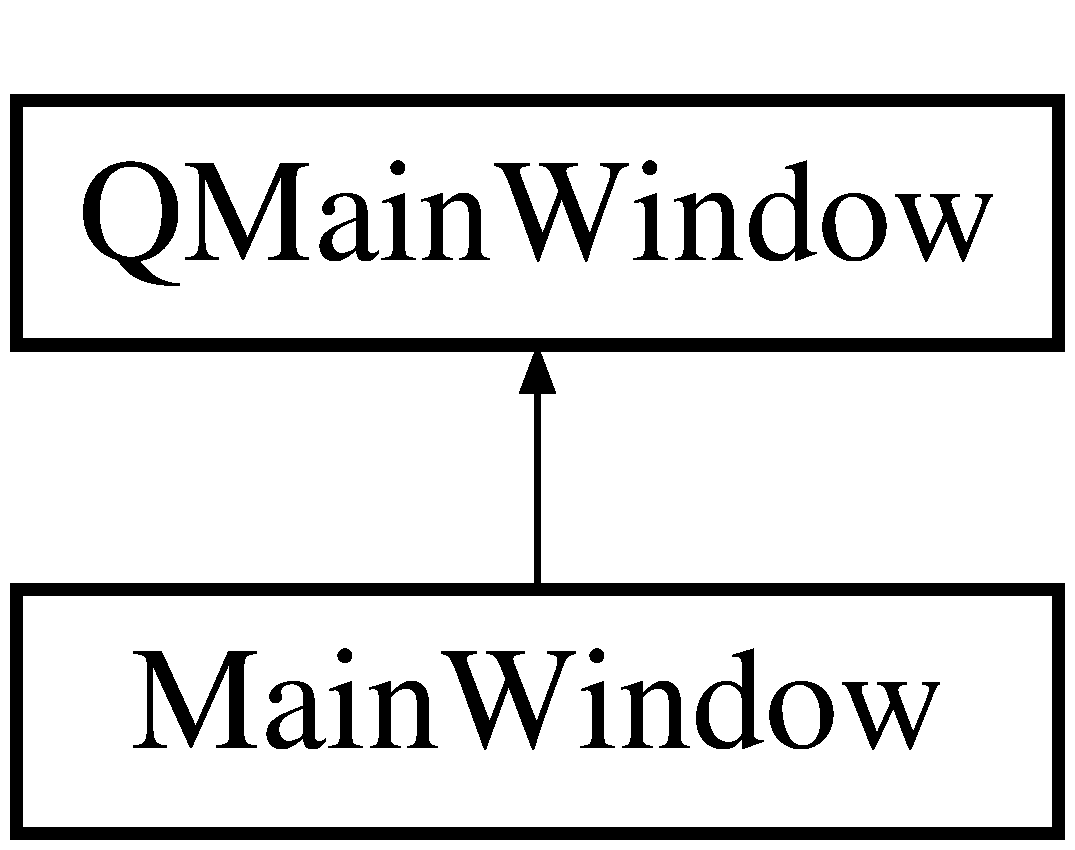
\includegraphics[height=2.000000cm]{classMainWindow}
\end{center}
\end{figure}
\subsection*{Public Member Functions}
\begin{DoxyCompactItemize}
\item 
{\footnotesize template$<$class Archive $>$ }\\void \hyperlink{classMainWindow_ab992ba5c7845b3642f6cba0771733bf0}{serialize} (Archive \&archive)
\item 
\hyperlink{classMainWindow_a8b244be8b7b7db1b08de2a2acb9409db}{Main\+Window} (Q\+Widget $\ast$parent=0)
\item 
\hyperlink{classMainWindow_ae98d00a93bc118200eeef9f9bba1dba7}{$\sim$\+Main\+Window} ()
\end{DoxyCompactItemize}


\subsection{Detailed Description}


Definition at line 33 of file mainwindow.\+h.



\subsection{Constructor \& Destructor Documentation}
\hypertarget{classMainWindow_a8b244be8b7b7db1b08de2a2acb9409db}{}\index{Main\+Window@{Main\+Window}!Main\+Window@{Main\+Window}}
\index{Main\+Window@{Main\+Window}!Main\+Window@{Main\+Window}}
\subsubsection[{Main\+Window}]{\setlength{\rightskip}{0pt plus 5cm}Main\+Window\+::\+Main\+Window (
\begin{DoxyParamCaption}
\item[{Q\+Widget $\ast$}]{parent = {\ttfamily 0}}
\end{DoxyParamCaption}
)\hspace{0.3cm}{\ttfamily [explicit]}}\label{classMainWindow_a8b244be8b7b7db1b08de2a2acb9409db}
Constructor 
\begin{DoxyParams}{Parameters}
{\em parent} & Parent widget \\
\hline
\end{DoxyParams}


Definition at line 38 of file mainwindow.\+cpp.

\hypertarget{classMainWindow_ae98d00a93bc118200eeef9f9bba1dba7}{}\index{Main\+Window@{Main\+Window}!````~Main\+Window@{$\sim$\+Main\+Window}}
\index{````~Main\+Window@{$\sim$\+Main\+Window}!Main\+Window@{Main\+Window}}
\subsubsection[{$\sim$\+Main\+Window}]{\setlength{\rightskip}{0pt plus 5cm}Main\+Window\+::$\sim$\+Main\+Window (
\begin{DoxyParamCaption}
{}
\end{DoxyParamCaption}
)}\label{classMainWindow_ae98d00a93bc118200eeef9f9bba1dba7}
Destructor 

Definition at line 147 of file mainwindow.\+cpp.



\subsection{Member Function Documentation}
\hypertarget{classMainWindow_ab992ba5c7845b3642f6cba0771733bf0}{}\index{Main\+Window@{Main\+Window}!serialize@{serialize}}
\index{serialize@{serialize}!Main\+Window@{Main\+Window}}
\subsubsection[{serialize}]{\setlength{\rightskip}{0pt plus 5cm}template$<$class Archive $>$ void Main\+Window\+::serialize (
\begin{DoxyParamCaption}
\item[{Archive \&}]{archive}
\end{DoxyParamCaption}
)\hspace{0.3cm}{\ttfamily [inline]}}\label{classMainWindow_ab992ba5c7845b3642f6cba0771733bf0}
C\+E\+R\+E\+A\+L serialization 

Definition at line 42 of file mainwindow.\+h.



The documentation for this class was generated from the following files\+:\begin{DoxyCompactItemize}
\item 
headers/\hyperlink{mainwindow_8h}{mainwindow.\+h}\item 
sources/\hyperlink{mainwindow_8cpp}{mainwindow.\+cpp}\end{DoxyCompactItemize}

\hypertarget{structObjectColor}{}\section{Object\+Color Struct Reference}
\label{structObjectColor}\index{Object\+Color@{Object\+Color}}
\subsection*{Public Member Functions}
\begin{DoxyCompactItemize}
\item 
\hypertarget{structObjectColor_ab2332614caf0d8db4aa5dfb5154e521c}{}{\footnotesize template$<$class Archive $>$ }\\void {\bfseries serialize} (Archive \&archive)\label{structObjectColor_ab2332614caf0d8db4aa5dfb5154e521c}

\item 
\hypertarget{structObjectColor_abc0870b5b57f7ddbd1c5b6c35440e7f0}{}{\bfseries Object\+Color} (int r, int g, int b)\label{structObjectColor_abc0870b5b57f7ddbd1c5b6c35440e7f0}

\end{DoxyCompactItemize}
\subsection*{Public Attributes}
\begin{DoxyCompactItemize}
\item 
\hypertarget{structObjectColor_a2f0370a2aa8ad4e90a0d679d72bdcd78}{}int {\bfseries r}\label{structObjectColor_a2f0370a2aa8ad4e90a0d679d72bdcd78}

\item 
\hypertarget{structObjectColor_a9b2f93ed12e3e03a30517574c5235981}{}int {\bfseries g}\label{structObjectColor_a9b2f93ed12e3e03a30517574c5235981}

\item 
\hypertarget{structObjectColor_ab0dee6c3856aa0ca9633a35271c78f4e}{}int {\bfseries b}\label{structObjectColor_ab0dee6c3856aa0ca9633a35271c78f4e}

\end{DoxyCompactItemize}


\subsection{Detailed Description}


Definition at line 40 of file selection.\+h.



The documentation for this struct was generated from the following file\+:\begin{DoxyCompactItemize}
\item 
headers/\hyperlink{selection_8h}{selection.\+h}\end{DoxyCompactItemize}

\hypertarget{structObjectShape}{}\section{Object\+Shape Struct Reference}
\label{structObjectShape}\index{Object\+Shape@{Object\+Shape}}
\subsection*{Static Public Attributes}
\begin{DoxyCompactItemize}
\item 
\hypertarget{structObjectShape_a37b224be8af923a9557b47179c608621}{}static const unsigned {\bfseries R\+E\+C\+T\+A\+N\+G\+L\+E} = 1\label{structObjectShape_a37b224be8af923a9557b47179c608621}

\item 
\hypertarget{structObjectShape_ab715c818a8afa39d34923ce0974e1328}{}static const unsigned {\bfseries E\+L\+L\+I\+P\+S\+E} = 2\label{structObjectShape_ab715c818a8afa39d34923ce0974e1328}

\end{DoxyCompactItemize}


\subsection{Detailed Description}


Definition at line 10 of file objectshape.\+h.



The documentation for this struct was generated from the following files\+:\begin{DoxyCompactItemize}
\item 
headers/\hyperlink{objectshape_8h}{objectshape.\+h}\item 
sources/\hyperlink{objectshape_8cpp}{objectshape.\+cpp}\end{DoxyCompactItemize}

\hypertarget{structOpenException}{}\section{Open\+Exception Struct Reference}
\label{structOpenException}\index{Open\+Exception@{Open\+Exception}}
Inheritance diagram for Open\+Exception\+:\begin{figure}[H]
\begin{center}
\leavevmode
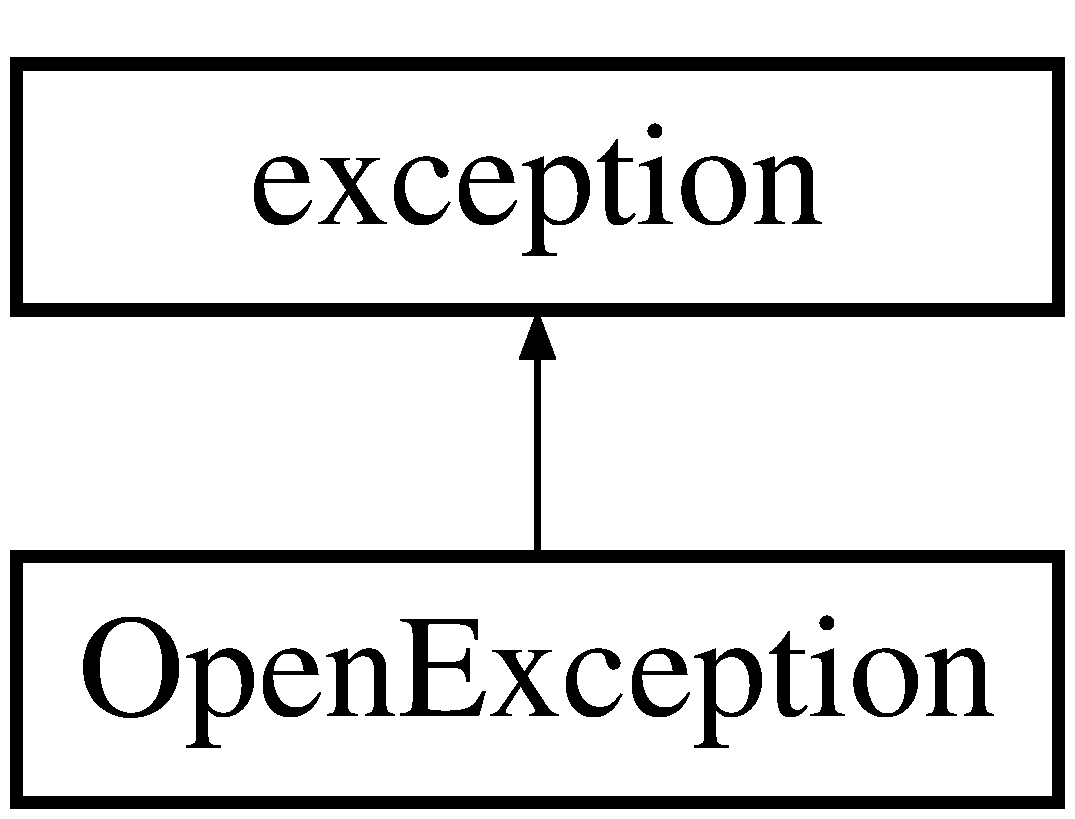
\includegraphics[height=2.000000cm]{structOpenException}
\end{center}
\end{figure}


\subsection{Detailed Description}


Definition at line 39 of file ffmpegplayer.\+h.



The documentation for this struct was generated from the following file\+:\begin{DoxyCompactItemize}
\item 
headers/\hyperlink{ffmpegplayer_8h}{ffmpegplayer.\+h}\end{DoxyCompactItemize}

\hypertarget{structOutputException}{}\section{Output\+Exception Struct Reference}
\label{structOutputException}\index{Output\+Exception@{Output\+Exception}}
Inheritance diagram for Output\+Exception\+:\begin{figure}[H]
\begin{center}
\leavevmode
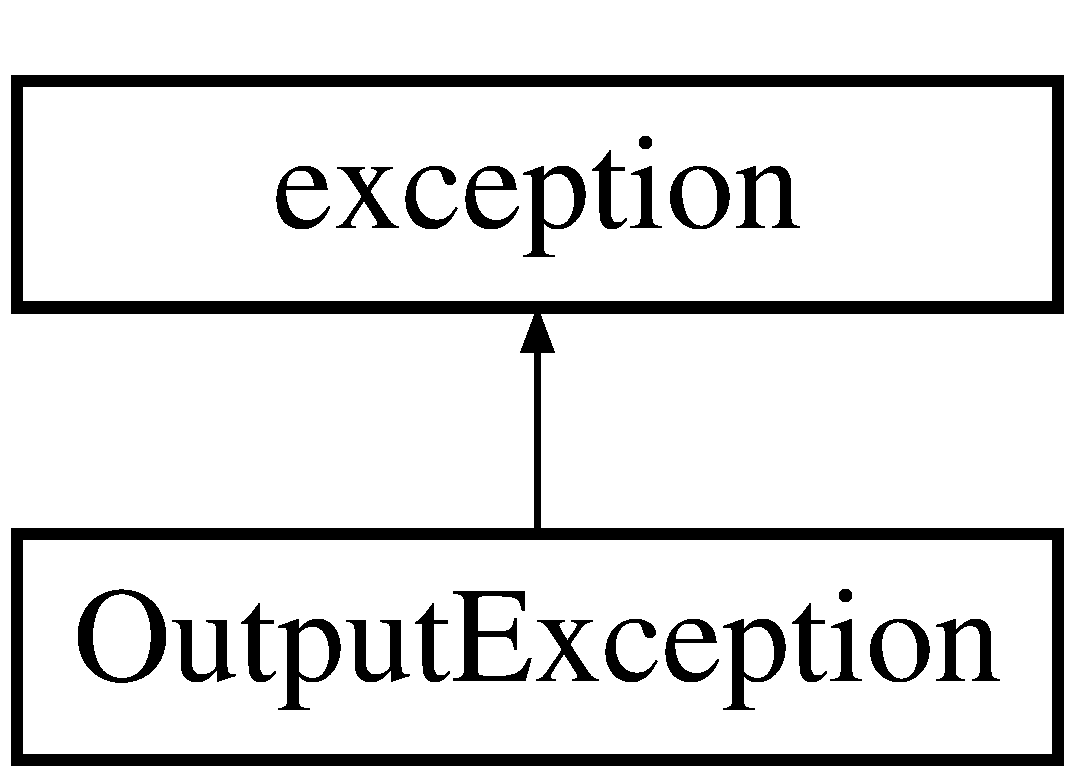
\includegraphics[height=2.000000cm]{structOutputException}
\end{center}
\end{figure}


\subsection{Detailed Description}


Definition at line 30 of file videotracker.\+h.



The documentation for this struct was generated from the following file\+:\begin{DoxyCompactItemize}
\item 
headers/\hyperlink{videotracker_8h}{videotracker.\+h}\end{DoxyCompactItemize}

\hypertarget{classPlayerSlider}{}\section{Player\+Slider Class Reference}
\label{classPlayerSlider}\index{Player\+Slider@{Player\+Slider}}
Inheritance diagram for Player\+Slider\+:\begin{figure}[H]
\begin{center}
\leavevmode
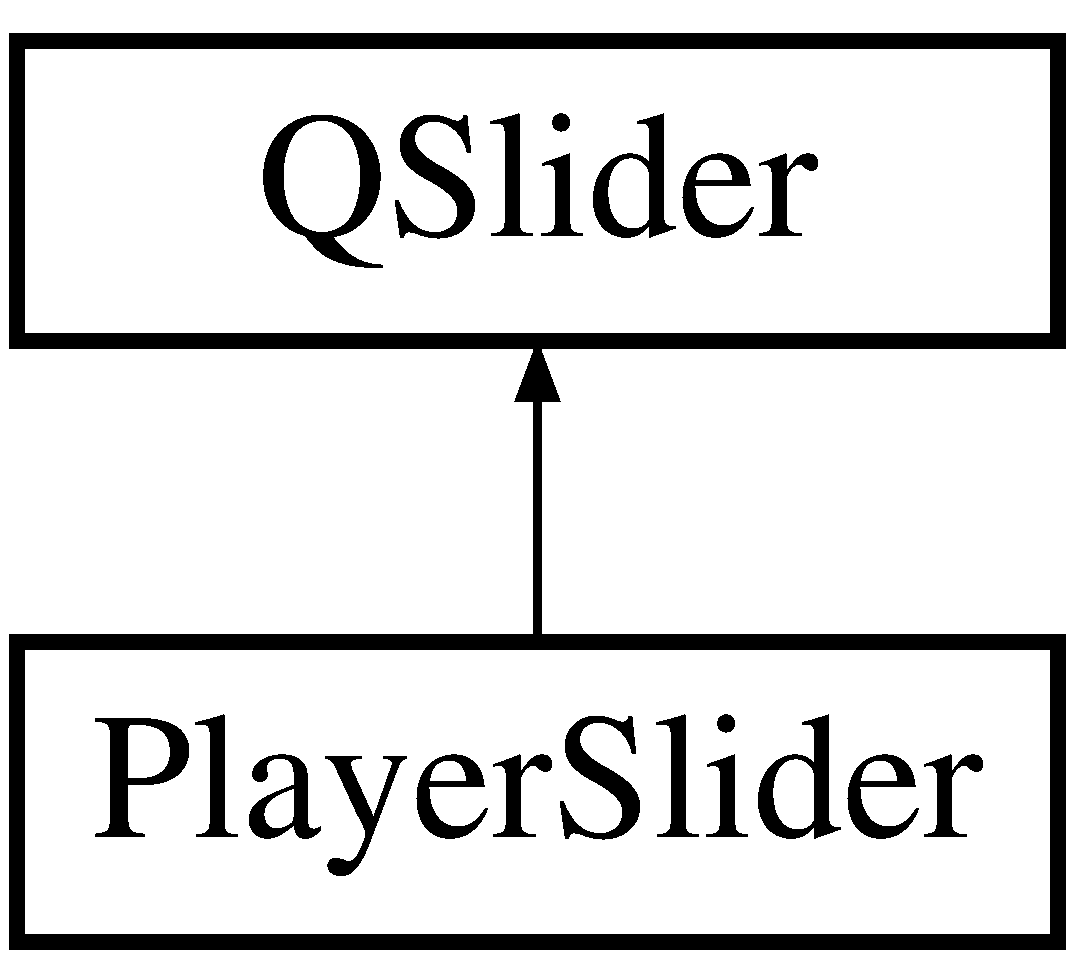
\includegraphics[height=2.000000cm]{classPlayerSlider}
\end{center}
\end{figure}
\subsection*{Signals}
\begin{DoxyCompactItemize}
\item 
void \hyperlink{classPlayerSlider_abef7cf0a30593a00702809005603eaf8}{clicked} (unsigned long)
\end{DoxyCompactItemize}
\subsection*{Public Member Functions}
\begin{DoxyCompactItemize}
\item 
\hyperlink{classPlayerSlider_a84733b1398e44defe971cc1c34ea7651}{Player\+Slider} (Q\+Widget $\ast$parent=0)
\item 
\hyperlink{classPlayerSlider_a02cf20dfe74926a7a1be1017e9c4e926}{$\sim$\+Player\+Slider} ()
\end{DoxyCompactItemize}
\subsection*{Protected Member Functions}
\begin{DoxyCompactItemize}
\item 
void \hyperlink{classPlayerSlider_a29c91c586725aee0822b966f701562c3}{mouse\+Release\+Event} (Q\+Mouse\+Event $\ast$event)
\end{DoxyCompactItemize}


\subsection{Detailed Description}


Definition at line 13 of file playerslider.\+h.



\subsection{Constructor \& Destructor Documentation}
\hypertarget{classPlayerSlider_a84733b1398e44defe971cc1c34ea7651}{}\index{Player\+Slider@{Player\+Slider}!Player\+Slider@{Player\+Slider}}
\index{Player\+Slider@{Player\+Slider}!Player\+Slider@{Player\+Slider}}
\subsubsection[{Player\+Slider}]{\setlength{\rightskip}{0pt plus 5cm}Player\+Slider\+::\+Player\+Slider (
\begin{DoxyParamCaption}
\item[{Q\+Widget $\ast$}]{parent = {\ttfamily 0}}
\end{DoxyParamCaption}
)\hspace{0.3cm}{\ttfamily [explicit]}}\label{classPlayerSlider_a84733b1398e44defe971cc1c34ea7651}
Constructor 
\begin{DoxyParams}{Parameters}
{\em parent} & Parent widget \\
\hline
\end{DoxyParams}


Definition at line 11 of file playerslider.\+cpp.

\hypertarget{classPlayerSlider_a02cf20dfe74926a7a1be1017e9c4e926}{}\index{Player\+Slider@{Player\+Slider}!````~Player\+Slider@{$\sim$\+Player\+Slider}}
\index{````~Player\+Slider@{$\sim$\+Player\+Slider}!Player\+Slider@{Player\+Slider}}
\subsubsection[{$\sim$\+Player\+Slider}]{\setlength{\rightskip}{0pt plus 5cm}Player\+Slider\+::$\sim$\+Player\+Slider (
\begin{DoxyParamCaption}
{}
\end{DoxyParamCaption}
)}\label{classPlayerSlider_a02cf20dfe74926a7a1be1017e9c4e926}
Destructor 

Definition at line 104 of file playerslider.\+cpp.



\subsection{Member Function Documentation}
\hypertarget{classPlayerSlider_abef7cf0a30593a00702809005603eaf8}{}\index{Player\+Slider@{Player\+Slider}!clicked@{clicked}}
\index{clicked@{clicked}!Player\+Slider@{Player\+Slider}}
\subsubsection[{clicked}]{\setlength{\rightskip}{0pt plus 5cm}void Player\+Slider\+::clicked (
\begin{DoxyParamCaption}
\item[{unsigned}]{long}
\end{DoxyParamCaption}
)\hspace{0.3cm}{\ttfamily [signal]}}\label{classPlayerSlider_abef7cf0a30593a00702809005603eaf8}
When a click is detected, this signal send a position of the click. 
\begin{DoxyParams}{Parameters}
{\em Position} & of the slider where the click was made \\
\hline
\end{DoxyParams}
\hypertarget{classPlayerSlider_a29c91c586725aee0822b966f701562c3}{}\index{Player\+Slider@{Player\+Slider}!mouse\+Release\+Event@{mouse\+Release\+Event}}
\index{mouse\+Release\+Event@{mouse\+Release\+Event}!Player\+Slider@{Player\+Slider}}
\subsubsection[{mouse\+Release\+Event}]{\setlength{\rightskip}{0pt plus 5cm}void Player\+Slider\+::mouse\+Release\+Event (
\begin{DoxyParamCaption}
\item[{Q\+Mouse\+Event $\ast$}]{event}
\end{DoxyParamCaption}
)\hspace{0.3cm}{\ttfamily [protected]}}\label{classPlayerSlider_a29c91c586725aee0822b966f701562c3}
Captures mouse release events to detect a mouse click that is processed and clicked signal is emitted. 
\begin{DoxyParams}{Parameters}
{\em event} & Mouse event\\
\hline
\end{DoxyParams}
void Player\+Slider\+::mouse\+Press\+Event(\+Q\+Mouse\+Event $\ast$event) \{ Q\+Slider mouse\+Press\+Event needs to be called so that signals slider\+Pressed with slider\+Moved are emitted correctly. It also sets flag Slider\+Down when the \char`\"{}controller\char`\"{} is pressed and therefore no further action is needed since the pressed position is the current one. Q\+Slider\+::mouse\+Press\+Event(event); if (is\+Slider\+Down()) return;

if (event-\/$>$button() == Qt\+::\+Left\+Button) \{ \begin{DoxyVerb}int position;
double value = 0; //0-1
if (orientation() == Qt::Horizontal)
    value = event->x() / static_cast<double>(width()-1);
else // ==Qt::Vertical
    value = event->y() / static_cast<double>(height()-1);
\end{DoxyVerb}


Position is more accurate when floor() is used at the beginning and ceil() at the end. if (value $<$ 0.\+3) position = floor(minimum() + (maximum()-\/minimum()) $\ast$ value); else if (value $>$ 0.\+7) position = ceil(minimum() + (maximum()-\/minimum()) $\ast$ value); else position = round(minimum() + (maximum()-\/minimum()) $\ast$ value);

emit slider\+Moved(position);

event-\/$>$accept(); \}

\} 

Definition at line 56 of file playerslider.\+cpp.



The documentation for this class was generated from the following files\+:\begin{DoxyCompactItemize}
\item 
headers/\hyperlink{playerslider_8h}{playerslider.\+h}\item 
sources/\hyperlink{playerslider_8cpp}{playerslider.\+cpp}\end{DoxyCompactItemize}

\hypertarget{structSelection}{}\section{Selection Struct Reference}
\label{structSelection}\index{Selection@{Selection}}
\subsection*{Public Member Functions}
\begin{DoxyCompactItemize}
\item 
\hypertarget{structSelection_adbb242e3a61e04da7460170dfbc2bae6}{}{\footnotesize template$<$class Archive $>$ }\\void {\bfseries serialize} (Archive \&archive)\label{structSelection_adbb242e3a61e04da7460170dfbc2bae6}

\item 
\hypertarget{structSelection_a7869a17657fdee2ddc601446776560c8}{}{\bfseries Selection} (int x, int y, int width, int height, int angle=0)\label{structSelection_a7869a17657fdee2ddc601446776560c8}

\end{DoxyCompactItemize}
\subsection*{Public Attributes}
\begin{DoxyCompactItemize}
\item 
\hypertarget{structSelection_aea07aa2d6e4ad8913e601a6be8fea52c}{}int {\bfseries x}\label{structSelection_aea07aa2d6e4ad8913e601a6be8fea52c}

\item 
\hypertarget{structSelection_ae95986151d57c8c4b06dadfe967b2a74}{}int {\bfseries y}\label{structSelection_ae95986151d57c8c4b06dadfe967b2a74}

\item 
\hypertarget{structSelection_ae11882f5ebb0a0ed08bfc903b174d253}{}int {\bfseries width}\label{structSelection_ae11882f5ebb0a0ed08bfc903b174d253}

\item 
\hypertarget{structSelection_a889204908783a2e132df34c001e4d40a}{}int {\bfseries height}\label{structSelection_a889204908783a2e132df34c001e4d40a}

\item 
\hypertarget{structSelection_a00964248804d5766816c6fed9ce67920}{}double {\bfseries angle}\label{structSelection_a00964248804d5766816c6fed9ce67920}

\end{DoxyCompactItemize}


\subsection{Detailed Description}


Definition at line 15 of file selection.\+h.



The documentation for this struct was generated from the following file\+:\begin{DoxyCompactItemize}
\item 
headers/\hyperlink{selection_8h}{selection.\+h}\end{DoxyCompactItemize}

\hypertarget{structTimeConversion_1_1Time}{}\section{Time\+Conversion\+:\+:Time Struct Reference}
\label{structTimeConversion_1_1Time}\index{Time\+Conversion\+::\+Time@{Time\+Conversion\+::\+Time}}
\subsection*{Public Attributes}
\begin{DoxyCompactItemize}
\item 
\hypertarget{structTimeConversion_1_1Time_af994b4dfc68913059d4b9f1e87c06a99}{}unsigned long {\bfseries raw}\label{structTimeConversion_1_1Time_af994b4dfc68913059d4b9f1e87c06a99}

\item 
\hypertarget{structTimeConversion_1_1Time_a622a32fbf330e9b9b8c71cba88b564f5}{}unsigned long {\bfseries hr}\label{structTimeConversion_1_1Time_a622a32fbf330e9b9b8c71cba88b564f5}

\item 
\hypertarget{structTimeConversion_1_1Time_acb711ae4dca8c51bffcc63e48e36a11d}{}unsigned long {\bfseries min}\label{structTimeConversion_1_1Time_acb711ae4dca8c51bffcc63e48e36a11d}

\item 
\hypertarget{structTimeConversion_1_1Time_a93153aa67ed078df258310b6b52804ae}{}unsigned long {\bfseries sec}\label{structTimeConversion_1_1Time_a93153aa67ed078df258310b6b52804ae}

\item 
\hypertarget{structTimeConversion_1_1Time_a4837e0e893a0b8be137662e655b87995}{}unsigned long {\bfseries ms}\label{structTimeConversion_1_1Time_a4837e0e893a0b8be137662e655b87995}

\end{DoxyCompactItemize}


\subsection{Detailed Description}


Definition at line 14 of file timelabel.\+h.



The documentation for this struct was generated from the following file\+:\begin{DoxyCompactItemize}
\item 
headers/\hyperlink{timelabel_8h}{timelabel.\+h}\end{DoxyCompactItemize}

\hypertarget{classTimeLabel}{}\section{Time\+Label Class Reference}
\label{classTimeLabel}\index{Time\+Label@{Time\+Label}}
Inheritance diagram for Time\+Label\+:\begin{figure}[H]
\begin{center}
\leavevmode
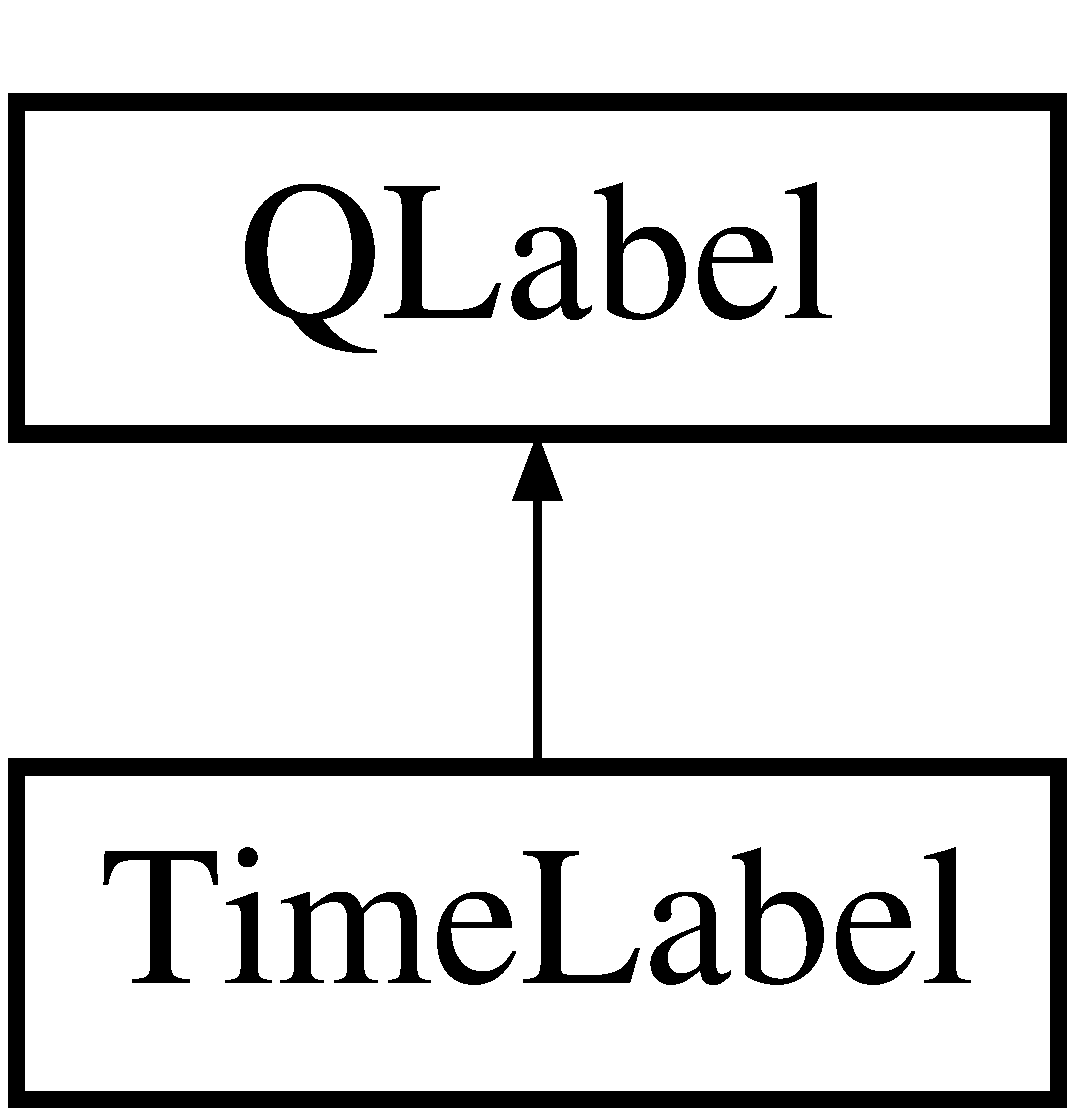
\includegraphics[height=2.000000cm]{classTimeLabel}
\end{center}
\end{figure}
\subsection*{Public Member Functions}
\begin{DoxyCompactItemize}
\item 
\hyperlink{classTimeLabel_ab5209722b07e051d8f491cd15a16d3a6}{Time\+Label} (Q\+Widget $\ast$parent=0)
\item 
\hyperlink{classTimeLabel_adf063e3753ec3518e8b2fb5ff3eed9e7}{$\sim$\+Time\+Label} ()
\item 
void \hyperlink{classTimeLabel_adcce5f44f60d58312c0a566b3dd0bf77}{set\+\_\+total\+\_\+time} (const unsigned long \&time)
\item 
void \hyperlink{classTimeLabel_a77ac5dbff384d73f672ef00dade79a54}{display\+\_\+time} (const unsigned long \&time, bool include\+Total=true)
\item 
void \hyperlink{classTimeLabel_a177fc7aff1b4257b947a9a174cd82362}{set\+\_\+frame\+\_\+count} (unsigned long frame\+Count)
\item 
void \hyperlink{classTimeLabel_ab92bd43ecd75617d5b5a187db72ed44b}{display\+\_\+frame\+\_\+num} (unsigned long frame\+Number, bool include\+Total=true)
\end{DoxyCompactItemize}


\subsection{Detailed Description}


Definition at line 33 of file timelabel.\+h.



\subsection{Constructor \& Destructor Documentation}
\hypertarget{classTimeLabel_ab5209722b07e051d8f491cd15a16d3a6}{}\index{Time\+Label@{Time\+Label}!Time\+Label@{Time\+Label}}
\index{Time\+Label@{Time\+Label}!Time\+Label@{Time\+Label}}
\subsubsection[{Time\+Label}]{\setlength{\rightskip}{0pt plus 5cm}Time\+Label\+::\+Time\+Label (
\begin{DoxyParamCaption}
\item[{Q\+Widget $\ast$}]{parent = {\ttfamily 0}}
\end{DoxyParamCaption}
)\hspace{0.3cm}{\ttfamily [explicit]}}\label{classTimeLabel_ab5209722b07e051d8f491cd15a16d3a6}
Constructor 
\begin{DoxyParams}{Parameters}
{\em parent} & Parent widget \\
\hline
\end{DoxyParams}


Definition at line 35 of file timelabel.\+cpp.

\hypertarget{classTimeLabel_adf063e3753ec3518e8b2fb5ff3eed9e7}{}\index{Time\+Label@{Time\+Label}!````~Time\+Label@{$\sim$\+Time\+Label}}
\index{````~Time\+Label@{$\sim$\+Time\+Label}!Time\+Label@{Time\+Label}}
\subsubsection[{$\sim$\+Time\+Label}]{\setlength{\rightskip}{0pt plus 5cm}Time\+Label\+::$\sim$\+Time\+Label (
\begin{DoxyParamCaption}
{}
\end{DoxyParamCaption}
)}\label{classTimeLabel_adf063e3753ec3518e8b2fb5ff3eed9e7}
Destructor 

Definition at line 42 of file timelabel.\+cpp.



\subsection{Member Function Documentation}
\hypertarget{classTimeLabel_ab92bd43ecd75617d5b5a187db72ed44b}{}\index{Time\+Label@{Time\+Label}!display\+\_\+frame\+\_\+num@{display\+\_\+frame\+\_\+num}}
\index{display\+\_\+frame\+\_\+num@{display\+\_\+frame\+\_\+num}!Time\+Label@{Time\+Label}}
\subsubsection[{display\+\_\+frame\+\_\+num}]{\setlength{\rightskip}{0pt plus 5cm}void Time\+Label\+::display\+\_\+frame\+\_\+num (
\begin{DoxyParamCaption}
\item[{unsigned long}]{frame\+Number, }
\item[{bool}]{include\+Total = {\ttfamily true}}
\end{DoxyParamCaption}
)}\label{classTimeLabel_ab92bd43ecd75617d5b5a187db72ed44b}
Displays given frame number with the total number of frames. 
\begin{DoxyParams}{Parameters}
{\em frame\+Number} & Displayed frame number \\
\hline
{\em include\+Total} & If true, total number of frames is also displayed. \\
\hline
\end{DoxyParams}


Definition at line 88 of file timelabel.\+cpp.

\hypertarget{classTimeLabel_a77ac5dbff384d73f672ef00dade79a54}{}\index{Time\+Label@{Time\+Label}!display\+\_\+time@{display\+\_\+time}}
\index{display\+\_\+time@{display\+\_\+time}!Time\+Label@{Time\+Label}}
\subsubsection[{display\+\_\+time}]{\setlength{\rightskip}{0pt plus 5cm}void Time\+Label\+::display\+\_\+time (
\begin{DoxyParamCaption}
\item[{const unsigned long \&}]{time, }
\item[{bool}]{include\+Total = {\ttfamily true}}
\end{DoxyParamCaption}
)}\label{classTimeLabel_a77ac5dbff384d73f672ef00dade79a54}
Displays given time position with the total time. 
\begin{DoxyParams}{Parameters}
{\em time} & Displayed time \\
\hline
{\em include\+Total} & If true, total length is also displayed. \\
\hline
\end{DoxyParams}


Definition at line 60 of file timelabel.\+cpp.

\hypertarget{classTimeLabel_a177fc7aff1b4257b947a9a174cd82362}{}\index{Time\+Label@{Time\+Label}!set\+\_\+frame\+\_\+count@{set\+\_\+frame\+\_\+count}}
\index{set\+\_\+frame\+\_\+count@{set\+\_\+frame\+\_\+count}!Time\+Label@{Time\+Label}}
\subsubsection[{set\+\_\+frame\+\_\+count}]{\setlength{\rightskip}{0pt plus 5cm}void Time\+Label\+::set\+\_\+frame\+\_\+count (
\begin{DoxyParamCaption}
\item[{unsigned long}]{frame\+Count}
\end{DoxyParamCaption}
)}\label{classTimeLabel_a177fc7aff1b4257b947a9a174cd82362}
Sets the total number of frames. 
\begin{DoxyParams}{Parameters}
{\em frame\+Count} & Number of frames \\
\hline
\end{DoxyParams}


Definition at line 83 of file timelabel.\+cpp.

\hypertarget{classTimeLabel_adcce5f44f60d58312c0a566b3dd0bf77}{}\index{Time\+Label@{Time\+Label}!set\+\_\+total\+\_\+time@{set\+\_\+total\+\_\+time}}
\index{set\+\_\+total\+\_\+time@{set\+\_\+total\+\_\+time}!Time\+Label@{Time\+Label}}
\subsubsection[{set\+\_\+total\+\_\+time}]{\setlength{\rightskip}{0pt plus 5cm}void Time\+Label\+::set\+\_\+total\+\_\+time (
\begin{DoxyParamCaption}
\item[{const unsigned long \&}]{time}
\end{DoxyParamCaption}
)}\label{classTimeLabel_adcce5f44f60d58312c0a566b3dd0bf77}
Sets the total video time. 
\begin{DoxyParams}{Parameters}
{\em time} & Time in milliseconds \\
\hline
\end{DoxyParams}


Definition at line 48 of file timelabel.\+cpp.



The documentation for this class was generated from the following files\+:\begin{DoxyCompactItemize}
\item 
headers/\hyperlink{timelabel_8h}{timelabel.\+h}\item 
sources/\hyperlink{timelabel_8cpp}{timelabel.\+cpp}\end{DoxyCompactItemize}

\hypertarget{classTrackedObject}{}\section{Tracked\+Object Class Reference}
\label{classTrackedObject}\index{Tracked\+Object@{Tracked\+Object}}
\subsection*{Public Member Functions}
\begin{DoxyCompactItemize}
\item 
{\footnotesize template$<$class Archive $>$ }\\void \hyperlink{classTrackedObject_ad6686a8c268d09f3c011d8fb33511550}{serialize} (Archive \&archive)
\item 
\hyperlink{classTrackedObject_ae5a9674bcce5464701811b6cd139dfaf}{Tracked\+Object} ()
\item 
\hyperlink{classTrackedObject_a30bc37fb38fd057d021c3dbe3f73b58e}{Tracked\+Object} (\hyperlink{structCharacteristics}{Characteristics} const \&appearance, std\+::string object\+Name, int64\+\_\+t initial\+Timestamp, \hyperlink{structSelection}{Selection} initial\+Position, unsigned long initial\+Time\+Position, unsigned long initial\+Frame\+Number, bool end\+Timestamp\+Set, int64\+\_\+t end\+Timestamp, unsigned long end\+Time\+Position, unsigned long end\+Frame\+Number)
\item 
\hyperlink{classTrackedObject_a3f9317e1ad294d3a391dfec7f7f926c0}{$\sim$\+Tracked\+Object} ()
\item 
void \hyperlink{classTrackedObject_a4cc6a3528caa148af9ab533a2bba587a}{add\+\_\+section} (int64\+\_\+t initial\+Timestamp, \hyperlink{structSelection}{Selection} const \&initial\+Position, unsigned long initial\+Time\+Position, unsigned long initial\+Frame\+Number)
\item 
bool \hyperlink{classTrackedObject_a89b293eacf57450551ecd30e768586be}{set\+\_\+trajectory\+\_\+section} (int64\+\_\+t new\+Timestamp, \hyperlink{structSelection}{Selection} position, unsigned long time\+Position, unsigned long frame\+Number)
\item 
bool \hyperlink{classTrackedObject_a0e8fd437e3e5af6d61d4cf3001463fa9}{change\+\_\+trajectory\+\_\+section} (int64\+\_\+t old\+Timestamp, int64\+\_\+t new\+Timestamp, \hyperlink{structSelection}{Selection} position, unsigned long time\+Position, unsigned long frame\+Number)
\item 
bool \hyperlink{classTrackedObject_a182387420b031f8c0c8a6dd102ebd10a}{change\+\_\+end\+\_\+frame} (bool set, int64\+\_\+t timestamp=0, unsigned long time\+Position=0, unsigned long frame\+Number=0)
\item 
void \hyperlink{classTrackedObject_a3f45315ecc8fcabeff15baefe19a5873}{change\+\_\+appearance} (\hyperlink{structCharacteristics}{Characteristics} const \&new\+Appearance)
\item 
\hyperlink{structCharacteristics}{Characteristics} \hyperlink{classTrackedObject_a798947c38b78d2c4da95cefa75a4d055}{get\+\_\+appearance} () const 
\item 
bool \hyperlink{classTrackedObject_af5b7f92c243707b5e2dfba099b50a3bd}{get\+\_\+position} (int64\+\_\+t timestamp, \hyperlink{structSelection}{Selection} \&tracked\+Position) const 
\item 
\hyperlink{structSelection}{Selection} \hyperlink{classTrackedObject_ae5dbab7c99f67ebfb2652ff01bfb34ff}{track\+\_\+next} (\hyperlink{classVideoFrame}{Video\+Frame} const $\ast$frame)
\item 
bool \hyperlink{classTrackedObject_a0ae55bacfcc78767b4d6ebe60a56db02}{draw\+\_\+mark} (cv\+::\+Mat \&frame, cv\+::\+Mat const \&original\+Frame, int64\+\_\+t timestamp) const 
\item 
std\+::map$<$ int64\+\_\+t, \hyperlink{structTrajectorySection}{Trajectory\+Section} $>$ const \& \hyperlink{classTrackedObject_af5fbc14bdee8d07311a9ba1ae9a32fd1}{get\+\_\+trajectory\+\_\+sections} () const 
\item 
std\+::map$<$ int64\+\_\+t, \hyperlink{structTrajectoryEntry}{Trajectory\+Entry} $>$ const \& \hyperlink{classTrackedObject_a1dc7353a75375f52a5c50296d77accb1}{get\+\_\+trajectory} () const 
\item 
int64\+\_\+t \hyperlink{classTrackedObject_a8a3294129b27947d40b2ccfa56bf578f}{get\+\_\+initial\+\_\+timestamp} () const 
\item 
int64\+\_\+t \hyperlink{classTrackedObject_a53303d656ec1a2cb664fdf3e9f4864af}{get\+\_\+end\+\_\+timestamp} () const 
\item 
unsigned long \hyperlink{classTrackedObject_a6899113e3ea7e025944e0ebb1fe38e93}{get\+\_\+end\+\_\+time\+\_\+position} () const 
\item 
unsigned long \hyperlink{classTrackedObject_acd0994794b432d6719196694f3718eda}{get\+\_\+end\+\_\+frame\+\_\+number} () const 
\item 
bool \hyperlink{classTrackedObject_a9dc31fd996676625f1ff96ce0d3e06ba}{get\+\_\+last\+\_\+processed\+\_\+timestamp} (int64\+\_\+t \&timestamp) const 
\item 
void \hyperlink{classTrackedObject_a000d56a6c6ac09ae5ee8b9e9fd016166}{set\+\_\+all\+\_\+processed} (bool processed)
\item 
bool \hyperlink{classTrackedObject_a4cbf70c8e11639d0f75065afbb167ab7}{is\+\_\+all\+\_\+processed} () const 
\item 
bool \hyperlink{classTrackedObject_af26454650654b9f390c1998e793dc3a8}{is\+\_\+end\+\_\+timestamp\+\_\+set} () const 
\item 
bool \hyperlink{classTrackedObject_a9429f18b7212b7e9e65604db5df9c209}{delete\+\_\+trajectory\+\_\+section} (int64\+\_\+t timestamp)
\item 
std\+::string \hyperlink{classTrackedObject_aacfdd49a2fc7f965e5368f21dc679957}{get\+\_\+name} () const 
\item 
bool \hyperlink{classTrackedObject_a166a4106e959819408d2d7a8b6c4308b}{set\+\_\+name} (std\+::string new\+Name)
\item 
void \hyperlink{classTrackedObject_ae33a79be587578620f63e426116846ff}{erase\+\_\+trajectory\+\_\+to\+\_\+comply} ()
\end{DoxyCompactItemize}


\subsection{Detailed Description}


Definition at line 113 of file trackedobject.\+h.



\subsection{Constructor \& Destructor Documentation}
\hypertarget{classTrackedObject_ae5a9674bcce5464701811b6cd139dfaf}{}\index{Tracked\+Object@{Tracked\+Object}!Tracked\+Object@{Tracked\+Object}}
\index{Tracked\+Object@{Tracked\+Object}!Tracked\+Object@{Tracked\+Object}}
\subsubsection[{Tracked\+Object}]{\setlength{\rightskip}{0pt plus 5cm}Tracked\+Object\+::\+Tracked\+Object (
\begin{DoxyParamCaption}
{}
\end{DoxyParamCaption}
)}\label{classTrackedObject_ae5a9674bcce5464701811b6cd139dfaf}
Constructor 

Definition at line 13 of file trackedobject.\+cpp.

\hypertarget{classTrackedObject_a30bc37fb38fd057d021c3dbe3f73b58e}{}\index{Tracked\+Object@{Tracked\+Object}!Tracked\+Object@{Tracked\+Object}}
\index{Tracked\+Object@{Tracked\+Object}!Tracked\+Object@{Tracked\+Object}}
\subsubsection[{Tracked\+Object}]{\setlength{\rightskip}{0pt plus 5cm}Tracked\+Object\+::\+Tracked\+Object (
\begin{DoxyParamCaption}
\item[{{\bf Characteristics} const \&}]{appearance, }
\item[{std\+::string}]{object\+Name, }
\item[{int64\+\_\+t}]{initial\+Timestamp, }
\item[{{\bf Selection}}]{initial\+Position, }
\item[{unsigned long}]{initial\+Time\+Position, }
\item[{unsigned long}]{initial\+Frame\+Number, }
\item[{bool}]{end\+Timestamp\+Set, }
\item[{int64\+\_\+t}]{end\+Timestamp, }
\item[{unsigned long}]{end\+Time\+Position, }
\item[{unsigned long}]{end\+Frame\+Number}
\end{DoxyParamCaption}
)}\label{classTrackedObject_a30bc37fb38fd057d021c3dbe3f73b58e}
Constructor 
\begin{DoxyParams}{Parameters}
{\em appearance} & Object appearance \\
\hline
{\em object\+Name} & Object name \\
\hline
{\em initial\+Timestamp} & Initial timestamp \\
\hline
{\em initial\+Position} & Initial object position \\
\hline
{\em initial\+Time\+Position} & Initial time position \\
\hline
{\em initial\+Frame\+Number} & Initial frame number \\
\hline
{\em end\+Timestamp\+Set} & Is end timestamp set? \\
\hline
{\em end\+Timestamp} & End timestamp \\
\hline
{\em end\+Time\+Position} & End time position \\
\hline
{\em end\+Frame\+Number} & End frame number \\
\hline
\end{DoxyParams}


Definition at line 22 of file trackedobject.\+cpp.

\hypertarget{classTrackedObject_a3f9317e1ad294d3a391dfec7f7f926c0}{}\index{Tracked\+Object@{Tracked\+Object}!````~Tracked\+Object@{$\sim$\+Tracked\+Object}}
\index{````~Tracked\+Object@{$\sim$\+Tracked\+Object}!Tracked\+Object@{Tracked\+Object}}
\subsubsection[{$\sim$\+Tracked\+Object}]{\setlength{\rightskip}{0pt plus 5cm}Tracked\+Object\+::$\sim$\+Tracked\+Object (
\begin{DoxyParamCaption}
{}
\end{DoxyParamCaption}
)}\label{classTrackedObject_a3f9317e1ad294d3a391dfec7f7f926c0}
Destructor if (tracking\+Algorithm) \{ // was it already initialized (by initialize\+\_\+section)? delete tracking\+Algorithm; tracking\+Algorithm = nullptr; \}

Definition at line 44 of file trackedobject.\+cpp.



\subsection{Member Function Documentation}
\hypertarget{classTrackedObject_a4cc6a3528caa148af9ab533a2bba587a}{}\index{Tracked\+Object@{Tracked\+Object}!add\+\_\+section@{add\+\_\+section}}
\index{add\+\_\+section@{add\+\_\+section}!Tracked\+Object@{Tracked\+Object}}
\subsubsection[{add\+\_\+section}]{\setlength{\rightskip}{0pt plus 5cm}void Tracked\+Object\+::add\+\_\+section (
\begin{DoxyParamCaption}
\item[{int64\+\_\+t}]{initial\+Timestamp, }
\item[{{\bf Selection} const \&}]{initial\+Position, }
\item[{unsigned long}]{initial\+Time\+Position, }
\item[{unsigned long}]{initial\+Frame\+Number}
\end{DoxyParamCaption}
)}\label{classTrackedObject_a4cc6a3528caa148af9ab533a2bba587a}
Adds a trajectory section of the object 
\begin{DoxyParams}{Parameters}
{\em initial\+Timestamp} & Initial timestamp of the section \\
\hline
{\em initial\+Position} & Object position at the initial timestamp \\
\hline
{\em initial\+Time\+Position} & Initial time position of the section \\
\hline
{\em initial\+Frame\+Number} & Initial frame number of the section \\
\hline
\end{DoxyParams}


Definition at line 65 of file trackedobject.\+cpp.

\hypertarget{classTrackedObject_a3f45315ecc8fcabeff15baefe19a5873}{}\index{Tracked\+Object@{Tracked\+Object}!change\+\_\+appearance@{change\+\_\+appearance}}
\index{change\+\_\+appearance@{change\+\_\+appearance}!Tracked\+Object@{Tracked\+Object}}
\subsubsection[{change\+\_\+appearance}]{\setlength{\rightskip}{0pt plus 5cm}void Tracked\+Object\+::change\+\_\+appearance (
\begin{DoxyParamCaption}
\item[{{\bf Characteristics} const \&}]{new\+Appearance}
\end{DoxyParamCaption}
)}\label{classTrackedObject_a3f45315ecc8fcabeff15baefe19a5873}
Changes appearance of the object. 
\begin{DoxyParams}{Parameters}
{\em new\+Appearance} & New appearance of the object \\
\hline
\end{DoxyParams}


Definition at line 342 of file trackedobject.\+cpp.

\hypertarget{classTrackedObject_a182387420b031f8c0c8a6dd102ebd10a}{}\index{Tracked\+Object@{Tracked\+Object}!change\+\_\+end\+\_\+frame@{change\+\_\+end\+\_\+frame}}
\index{change\+\_\+end\+\_\+frame@{change\+\_\+end\+\_\+frame}!Tracked\+Object@{Tracked\+Object}}
\subsubsection[{change\+\_\+end\+\_\+frame}]{\setlength{\rightskip}{0pt plus 5cm}bool Tracked\+Object\+::change\+\_\+end\+\_\+frame (
\begin{DoxyParamCaption}
\item[{bool}]{set, }
\item[{int64\+\_\+t}]{timestamp = {\ttfamily 0}, }
\item[{unsigned long}]{time\+Position = {\ttfamily 0}, }
\item[{unsigned long}]{frame\+Number = {\ttfamily 0}}
\end{DoxyParamCaption}
)}\label{classTrackedObject_a182387420b031f8c0c8a6dd102ebd10a}
Changes the end frame of the object. 
\begin{DoxyParams}{Parameters}
{\em set} & Set / unset last frame \\
\hline
{\em timestamp} & Timestamp of the last frame \\
\hline
{\em time\+Position} & Time position of the last frame \\
\hline
{\em frame\+Number} & Frame number of the last frame \\
\hline
\end{DoxyParams}
\begin{DoxyReturn}{Returns}
True if successful 
\end{DoxyReturn}


Definition at line 274 of file trackedobject.\+cpp.

\hypertarget{classTrackedObject_a0e8fd437e3e5af6d61d4cf3001463fa9}{}\index{Tracked\+Object@{Tracked\+Object}!change\+\_\+trajectory\+\_\+section@{change\+\_\+trajectory\+\_\+section}}
\index{change\+\_\+trajectory\+\_\+section@{change\+\_\+trajectory\+\_\+section}!Tracked\+Object@{Tracked\+Object}}
\subsubsection[{change\+\_\+trajectory\+\_\+section}]{\setlength{\rightskip}{0pt plus 5cm}bool Tracked\+Object\+::change\+\_\+trajectory\+\_\+section (
\begin{DoxyParamCaption}
\item[{int64\+\_\+t}]{old\+Timestamp, }
\item[{int64\+\_\+t}]{new\+Timestamp, }
\item[{{\bf Selection}}]{position, }
\item[{unsigned long}]{time\+Position, }
\item[{unsigned long}]{frame\+Number}
\end{DoxyParamCaption}
)}\label{classTrackedObject_a0e8fd437e3e5af6d61d4cf3001463fa9}
Changes a trajectory section of the object. 
\begin{DoxyParams}{Parameters}
{\em old\+Timestamp} & Old timestamp of the section \\
\hline
{\em new\+Timestamp} & New timestamp of the section \\
\hline
{\em position} & Object position at the first frame of the section \\
\hline
{\em time\+Position} & Time position of the section \\
\hline
{\em frame\+Number} & Frame number of the section \\
\hline
\end{DoxyParams}
\begin{DoxyReturn}{Returns}
True if successful 
\end{DoxyReturn}


Definition at line 144 of file trackedobject.\+cpp.

\hypertarget{classTrackedObject_a9429f18b7212b7e9e65604db5df9c209}{}\index{Tracked\+Object@{Tracked\+Object}!delete\+\_\+trajectory\+\_\+section@{delete\+\_\+trajectory\+\_\+section}}
\index{delete\+\_\+trajectory\+\_\+section@{delete\+\_\+trajectory\+\_\+section}!Tracked\+Object@{Tracked\+Object}}
\subsubsection[{delete\+\_\+trajectory\+\_\+section}]{\setlength{\rightskip}{0pt plus 5cm}bool Tracked\+Object\+::delete\+\_\+trajectory\+\_\+section (
\begin{DoxyParamCaption}
\item[{int64\+\_\+t}]{timestamp}
\end{DoxyParamCaption}
)}\label{classTrackedObject_a9429f18b7212b7e9e65604db5df9c209}
Deletes a trajectory section. 
\begin{DoxyParams}{Parameters}
{\em timestamp} & Trajectory section to be deleted begins at this timestamp \\
\hline
\end{DoxyParams}
\begin{DoxyReturn}{Returns}
True if successful 
\end{DoxyReturn}


Definition at line 223 of file trackedobject.\+cpp.

\hypertarget{classTrackedObject_a0ae55bacfcc78767b4d6ebe60a56db02}{}\index{Tracked\+Object@{Tracked\+Object}!draw\+\_\+mark@{draw\+\_\+mark}}
\index{draw\+\_\+mark@{draw\+\_\+mark}!Tracked\+Object@{Tracked\+Object}}
\subsubsection[{draw\+\_\+mark}]{\setlength{\rightskip}{0pt plus 5cm}bool Tracked\+Object\+::draw\+\_\+mark (
\begin{DoxyParamCaption}
\item[{cv\+::\+Mat \&}]{frame, }
\item[{cv\+::\+Mat const \&}]{original\+Frame, }
\item[{int64\+\_\+t}]{timestamp}
\end{DoxyParamCaption}
) const}\label{classTrackedObject_a0ae55bacfcc78767b4d6ebe60a56db02}
Draws mark of the object in a frame. 
\begin{DoxyParams}{Parameters}
{\em frame} & Frame for drawing \\
\hline
{\em original\+Frame} & Original frame \\
\hline
{\em timestamp} & Timestamp of the frame \\
\hline
\end{DoxyParams}
\begin{DoxyReturn}{Returns}
True if successful 
\end{DoxyReturn}


Definition at line 445 of file trackedobject.\+cpp.

\hypertarget{classTrackedObject_ae33a79be587578620f63e426116846ff}{}\index{Tracked\+Object@{Tracked\+Object}!erase\+\_\+trajectory\+\_\+to\+\_\+comply@{erase\+\_\+trajectory\+\_\+to\+\_\+comply}}
\index{erase\+\_\+trajectory\+\_\+to\+\_\+comply@{erase\+\_\+trajectory\+\_\+to\+\_\+comply}!Tracked\+Object@{Tracked\+Object}}
\subsubsection[{erase\+\_\+trajectory\+\_\+to\+\_\+comply}]{\setlength{\rightskip}{0pt plus 5cm}void Tracked\+Object\+::erase\+\_\+trajectory\+\_\+to\+\_\+comply (
\begin{DoxyParamCaption}
{}
\end{DoxyParamCaption}
)}\label{classTrackedObject_ae33a79be587578620f63e426116846ff}
Erases a part of the computed trajectory. This is necessary after deserialization (with C\+E\+R\+E\+A\+L) as \hyperlink{classTrackedObject_ae5dbab7c99f67ebfb2652ff01bfb34ff}{track\+\_\+next()} initializes correct sections only when the trajectory\textquotesingle{}s last frame is the last frame of the previous section. 

Definition at line 631 of file trackedobject.\+cpp.

\hypertarget{classTrackedObject_a798947c38b78d2c4da95cefa75a4d055}{}\index{Tracked\+Object@{Tracked\+Object}!get\+\_\+appearance@{get\+\_\+appearance}}
\index{get\+\_\+appearance@{get\+\_\+appearance}!Tracked\+Object@{Tracked\+Object}}
\subsubsection[{get\+\_\+appearance}]{\setlength{\rightskip}{0pt plus 5cm}{\bf Characteristics} Tracked\+Object\+::get\+\_\+appearance (
\begin{DoxyParamCaption}
{}
\end{DoxyParamCaption}
) const}\label{classTrackedObject_a798947c38b78d2c4da95cefa75a4d055}
Returns appearance of the object. \begin{DoxyReturn}{Returns}
Object appearance 
\end{DoxyReturn}


Definition at line 347 of file trackedobject.\+cpp.

\hypertarget{classTrackedObject_acd0994794b432d6719196694f3718eda}{}\index{Tracked\+Object@{Tracked\+Object}!get\+\_\+end\+\_\+frame\+\_\+number@{get\+\_\+end\+\_\+frame\+\_\+number}}
\index{get\+\_\+end\+\_\+frame\+\_\+number@{get\+\_\+end\+\_\+frame\+\_\+number}!Tracked\+Object@{Tracked\+Object}}
\subsubsection[{get\+\_\+end\+\_\+frame\+\_\+number}]{\setlength{\rightskip}{0pt plus 5cm}unsigned long Tracked\+Object\+::get\+\_\+end\+\_\+frame\+\_\+number (
\begin{DoxyParamCaption}
{}
\end{DoxyParamCaption}
) const}\label{classTrackedObject_acd0994794b432d6719196694f3718eda}
Returns end frame number. \begin{DoxyReturn}{Returns}
End frame number 
\end{DoxyReturn}


Definition at line 570 of file trackedobject.\+cpp.

\hypertarget{classTrackedObject_a6899113e3ea7e025944e0ebb1fe38e93}{}\index{Tracked\+Object@{Tracked\+Object}!get\+\_\+end\+\_\+time\+\_\+position@{get\+\_\+end\+\_\+time\+\_\+position}}
\index{get\+\_\+end\+\_\+time\+\_\+position@{get\+\_\+end\+\_\+time\+\_\+position}!Tracked\+Object@{Tracked\+Object}}
\subsubsection[{get\+\_\+end\+\_\+time\+\_\+position}]{\setlength{\rightskip}{0pt plus 5cm}unsigned long Tracked\+Object\+::get\+\_\+end\+\_\+time\+\_\+position (
\begin{DoxyParamCaption}
{}
\end{DoxyParamCaption}
) const}\label{classTrackedObject_a6899113e3ea7e025944e0ebb1fe38e93}
Returns end time position. \begin{DoxyReturn}{Returns}
End time position 
\end{DoxyReturn}


Definition at line 565 of file trackedobject.\+cpp.

\hypertarget{classTrackedObject_a53303d656ec1a2cb664fdf3e9f4864af}{}\index{Tracked\+Object@{Tracked\+Object}!get\+\_\+end\+\_\+timestamp@{get\+\_\+end\+\_\+timestamp}}
\index{get\+\_\+end\+\_\+timestamp@{get\+\_\+end\+\_\+timestamp}!Tracked\+Object@{Tracked\+Object}}
\subsubsection[{get\+\_\+end\+\_\+timestamp}]{\setlength{\rightskip}{0pt plus 5cm}int64\+\_\+t Tracked\+Object\+::get\+\_\+end\+\_\+timestamp (
\begin{DoxyParamCaption}
{}
\end{DoxyParamCaption}
) const}\label{classTrackedObject_a53303d656ec1a2cb664fdf3e9f4864af}
Returns end timestamp. \begin{DoxyReturn}{Returns}
End timestamp 
\end{DoxyReturn}


Definition at line 560 of file trackedobject.\+cpp.

\hypertarget{classTrackedObject_a8a3294129b27947d40b2ccfa56bf578f}{}\index{Tracked\+Object@{Tracked\+Object}!get\+\_\+initial\+\_\+timestamp@{get\+\_\+initial\+\_\+timestamp}}
\index{get\+\_\+initial\+\_\+timestamp@{get\+\_\+initial\+\_\+timestamp}!Tracked\+Object@{Tracked\+Object}}
\subsubsection[{get\+\_\+initial\+\_\+timestamp}]{\setlength{\rightskip}{0pt plus 5cm}int64\+\_\+t Tracked\+Object\+::get\+\_\+initial\+\_\+timestamp (
\begin{DoxyParamCaption}
{}
\end{DoxyParamCaption}
) const}\label{classTrackedObject_a8a3294129b27947d40b2ccfa56bf578f}
Returns initial timestamp. \begin{DoxyReturn}{Returns}
initial timestamp 
\end{DoxyReturn}


Definition at line 555 of file trackedobject.\+cpp.

\hypertarget{classTrackedObject_a9dc31fd996676625f1ff96ce0d3e06ba}{}\index{Tracked\+Object@{Tracked\+Object}!get\+\_\+last\+\_\+processed\+\_\+timestamp@{get\+\_\+last\+\_\+processed\+\_\+timestamp}}
\index{get\+\_\+last\+\_\+processed\+\_\+timestamp@{get\+\_\+last\+\_\+processed\+\_\+timestamp}!Tracked\+Object@{Tracked\+Object}}
\subsubsection[{get\+\_\+last\+\_\+processed\+\_\+timestamp}]{\setlength{\rightskip}{0pt plus 5cm}bool Tracked\+Object\+::get\+\_\+last\+\_\+processed\+\_\+timestamp (
\begin{DoxyParamCaption}
\item[{int64\+\_\+t \&}]{timestamp}
\end{DoxyParamCaption}
) const}\label{classTrackedObject_a9dc31fd996676625f1ff96ce0d3e06ba}
Returns last processed timestamp. 
\begin{DoxyParams}{Parameters}
{\em timestamp} & Returned last processed timestamp \\
\hline
\end{DoxyParams}
\begin{DoxyReturn}{Returns}
Is returned timestamp valid? 
\end{DoxyReturn}


Definition at line 578 of file trackedobject.\+cpp.

\hypertarget{classTrackedObject_aacfdd49a2fc7f965e5368f21dc679957}{}\index{Tracked\+Object@{Tracked\+Object}!get\+\_\+name@{get\+\_\+name}}
\index{get\+\_\+name@{get\+\_\+name}!Tracked\+Object@{Tracked\+Object}}
\subsubsection[{get\+\_\+name}]{\setlength{\rightskip}{0pt plus 5cm}std\+::string Tracked\+Object\+::get\+\_\+name (
\begin{DoxyParamCaption}
{}
\end{DoxyParamCaption}
) const}\label{classTrackedObject_aacfdd49a2fc7f965e5368f21dc679957}
Returns name of the object. \begin{DoxyReturn}{Returns}
Object name 
\end{DoxyReturn}


Definition at line 619 of file trackedobject.\+cpp.

\hypertarget{classTrackedObject_af5b7f92c243707b5e2dfba099b50a3bd}{}\index{Tracked\+Object@{Tracked\+Object}!get\+\_\+position@{get\+\_\+position}}
\index{get\+\_\+position@{get\+\_\+position}!Tracked\+Object@{Tracked\+Object}}
\subsubsection[{get\+\_\+position}]{\setlength{\rightskip}{0pt plus 5cm}bool Tracked\+Object\+::get\+\_\+position (
\begin{DoxyParamCaption}
\item[{int64\+\_\+t}]{timestamp, }
\item[{{\bf Selection} \&}]{tracked\+Position}
\end{DoxyParamCaption}
) const}\label{classTrackedObject_af5b7f92c243707b5e2dfba099b50a3bd}
Returns position of the object at frame with given timestamp. 
\begin{DoxyParams}{Parameters}
{\em timestamp} & Frame timestamp \\
\hline
{\em tracked\+Position} & Returned object position \\
\hline
\end{DoxyParams}
\begin{DoxyReturn}{Returns}
False if trajectory with given timestamp does not exist, otherwise true. 
\end{DoxyReturn}


Definition at line 433 of file trackedobject.\+cpp.

\hypertarget{classTrackedObject_a1dc7353a75375f52a5c50296d77accb1}{}\index{Tracked\+Object@{Tracked\+Object}!get\+\_\+trajectory@{get\+\_\+trajectory}}
\index{get\+\_\+trajectory@{get\+\_\+trajectory}!Tracked\+Object@{Tracked\+Object}}
\subsubsection[{get\+\_\+trajectory}]{\setlength{\rightskip}{0pt plus 5cm}std\+::map$<$ int64\+\_\+t, {\bf Trajectory\+Entry} $>$ const \& Tracked\+Object\+::get\+\_\+trajectory (
\begin{DoxyParamCaption}
{}
\end{DoxyParamCaption}
) const}\label{classTrackedObject_a1dc7353a75375f52a5c50296d77accb1}
Returns computed trajectory of the object. \begin{DoxyReturn}{Returns}
Trajectory of the object 
\end{DoxyReturn}


Definition at line 550 of file trackedobject.\+cpp.

\hypertarget{classTrackedObject_af5fbc14bdee8d07311a9ba1ae9a32fd1}{}\index{Tracked\+Object@{Tracked\+Object}!get\+\_\+trajectory\+\_\+sections@{get\+\_\+trajectory\+\_\+sections}}
\index{get\+\_\+trajectory\+\_\+sections@{get\+\_\+trajectory\+\_\+sections}!Tracked\+Object@{Tracked\+Object}}
\subsubsection[{get\+\_\+trajectory\+\_\+sections}]{\setlength{\rightskip}{0pt plus 5cm}std\+::map$<$ int64\+\_\+t, {\bf Trajectory\+Section} $>$ const \& Tracked\+Object\+::get\+\_\+trajectory\+\_\+sections (
\begin{DoxyParamCaption}
{}
\end{DoxyParamCaption}
) const}\label{classTrackedObject_af5fbc14bdee8d07311a9ba1ae9a32fd1}
Returns trajectory sections of the object. \begin{DoxyReturn}{Returns}
Trajectory section of the object 
\end{DoxyReturn}


Definition at line 545 of file trackedobject.\+cpp.

\hypertarget{classTrackedObject_a4cbf70c8e11639d0f75065afbb167ab7}{}\index{Tracked\+Object@{Tracked\+Object}!is\+\_\+all\+\_\+processed@{is\+\_\+all\+\_\+processed}}
\index{is\+\_\+all\+\_\+processed@{is\+\_\+all\+\_\+processed}!Tracked\+Object@{Tracked\+Object}}
\subsubsection[{is\+\_\+all\+\_\+processed}]{\setlength{\rightskip}{0pt plus 5cm}bool Tracked\+Object\+::is\+\_\+all\+\_\+processed (
\begin{DoxyParamCaption}
{}
\end{DoxyParamCaption}
) const}\label{classTrackedObject_a4cbf70c8e11639d0f75065afbb167ab7}
Returns whether all trajectory is processed. \begin{DoxyReturn}{Returns}
Is all trajectory processed? 
\end{DoxyReturn}


Definition at line 609 of file trackedobject.\+cpp.

\hypertarget{classTrackedObject_af26454650654b9f390c1998e793dc3a8}{}\index{Tracked\+Object@{Tracked\+Object}!is\+\_\+end\+\_\+timestamp\+\_\+set@{is\+\_\+end\+\_\+timestamp\+\_\+set}}
\index{is\+\_\+end\+\_\+timestamp\+\_\+set@{is\+\_\+end\+\_\+timestamp\+\_\+set}!Tracked\+Object@{Tracked\+Object}}
\subsubsection[{is\+\_\+end\+\_\+timestamp\+\_\+set}]{\setlength{\rightskip}{0pt plus 5cm}bool Tracked\+Object\+::is\+\_\+end\+\_\+timestamp\+\_\+set (
\begin{DoxyParamCaption}
{}
\end{DoxyParamCaption}
) const}\label{classTrackedObject_af26454650654b9f390c1998e793dc3a8}
Returns whether the end timestamp is set. \begin{DoxyReturn}{Returns}
Is end timestamp set? 
\end{DoxyReturn}


Definition at line 614 of file trackedobject.\+cpp.

\hypertarget{classTrackedObject_ad6686a8c268d09f3c011d8fb33511550}{}\index{Tracked\+Object@{Tracked\+Object}!serialize@{serialize}}
\index{serialize@{serialize}!Tracked\+Object@{Tracked\+Object}}
\subsubsection[{serialize}]{\setlength{\rightskip}{0pt plus 5cm}template$<$class Archive $>$ void Tracked\+Object\+::serialize (
\begin{DoxyParamCaption}
\item[{Archive \&}]{archive}
\end{DoxyParamCaption}
)\hspace{0.3cm}{\ttfamily [inline]}}\label{classTrackedObject_ad6686a8c268d09f3c011d8fb33511550}
C\+E\+R\+E\+A\+L serialization 

Definition at line 121 of file trackedobject.\+h.

\hypertarget{classTrackedObject_a000d56a6c6ac09ae5ee8b9e9fd016166}{}\index{Tracked\+Object@{Tracked\+Object}!set\+\_\+all\+\_\+processed@{set\+\_\+all\+\_\+processed}}
\index{set\+\_\+all\+\_\+processed@{set\+\_\+all\+\_\+processed}!Tracked\+Object@{Tracked\+Object}}
\subsubsection[{set\+\_\+all\+\_\+processed}]{\setlength{\rightskip}{0pt plus 5cm}void Tracked\+Object\+::set\+\_\+all\+\_\+processed (
\begin{DoxyParamCaption}
\item[{bool}]{processed}
\end{DoxyParamCaption}
)}\label{classTrackedObject_a000d56a6c6ac09ae5ee8b9e9fd016166}
Sets value of the flag saying whether all trajectory is processed. 
\begin{DoxyParams}{Parameters}
{\em processed} & Set / unset \\
\hline
\end{DoxyParams}


Definition at line 591 of file trackedobject.\+cpp.

\hypertarget{classTrackedObject_a166a4106e959819408d2d7a8b6c4308b}{}\index{Tracked\+Object@{Tracked\+Object}!set\+\_\+name@{set\+\_\+name}}
\index{set\+\_\+name@{set\+\_\+name}!Tracked\+Object@{Tracked\+Object}}
\subsubsection[{set\+\_\+name}]{\setlength{\rightskip}{0pt plus 5cm}bool Tracked\+Object\+::set\+\_\+name (
\begin{DoxyParamCaption}
\item[{std\+::string}]{new\+Name}
\end{DoxyParamCaption}
)}\label{classTrackedObject_a166a4106e959819408d2d7a8b6c4308b}
Sets name of the object. 
\begin{DoxyParams}{Parameters}
{\em new\+Name} & New object name \\
\hline
\end{DoxyParams}
\begin{DoxyReturn}{Returns}
True if successful 
\end{DoxyReturn}


Definition at line 624 of file trackedobject.\+cpp.

\hypertarget{classTrackedObject_a89b293eacf57450551ecd30e768586be}{}\index{Tracked\+Object@{Tracked\+Object}!set\+\_\+trajectory\+\_\+section@{set\+\_\+trajectory\+\_\+section}}
\index{set\+\_\+trajectory\+\_\+section@{set\+\_\+trajectory\+\_\+section}!Tracked\+Object@{Tracked\+Object}}
\subsubsection[{set\+\_\+trajectory\+\_\+section}]{\setlength{\rightskip}{0pt plus 5cm}bool Tracked\+Object\+::set\+\_\+trajectory\+\_\+section (
\begin{DoxyParamCaption}
\item[{int64\+\_\+t}]{new\+Timestamp, }
\item[{{\bf Selection}}]{position, }
\item[{unsigned long}]{time\+Position, }
\item[{unsigned long}]{frame\+Number}
\end{DoxyParamCaption}
)}\label{classTrackedObject_a89b293eacf57450551ecd30e768586be}
Sets a trajectory section of the object. 
\begin{DoxyParams}{Parameters}
{\em new\+Timestamp} & New timestamp of the section \\
\hline
{\em position} & Object position at the first frame of the section \\
\hline
{\em time\+Position} & Time position of the section \\
\hline
{\em frame\+Number} & Frame number of the section \\
\hline
\end{DoxyParams}
\begin{DoxyReturn}{Returns}
True if successful 
\end{DoxyReturn}


Definition at line 75 of file trackedobject.\+cpp.

\hypertarget{classTrackedObject_ae5dbab7c99f67ebfb2652ff01bfb34ff}{}\index{Tracked\+Object@{Tracked\+Object}!track\+\_\+next@{track\+\_\+next}}
\index{track\+\_\+next@{track\+\_\+next}!Tracked\+Object@{Tracked\+Object}}
\subsubsection[{track\+\_\+next}]{\setlength{\rightskip}{0pt plus 5cm}{\bf Selection} Tracked\+Object\+::track\+\_\+next (
\begin{DoxyParamCaption}
\item[{{\bf Video\+Frame} const $\ast$}]{frame}
\end{DoxyParamCaption}
)}\label{classTrackedObject_ae5dbab7c99f67ebfb2652ff01bfb34ff}
Computes position of the object in the next frame. 
\begin{DoxyParams}{Parameters}
{\em frame} & Next frame \\
\hline
\end{DoxyParams}
\begin{DoxyReturn}{Returns}
Tracked object position 
\end{DoxyReturn}


Definition at line 356 of file trackedobject.\+cpp.



The documentation for this class was generated from the following files\+:\begin{DoxyCompactItemize}
\item 
headers/\hyperlink{trackedobject_8h}{trackedobject.\+h}\item 
sources/\hyperlink{trackedobject_8cpp}{trackedobject.\+cpp}\end{DoxyCompactItemize}

\hypertarget{classTrackingAlgorithm}{}\section{Tracking\+Algorithm Class Reference}
\label{classTrackingAlgorithm}\index{Tracking\+Algorithm@{Tracking\+Algorithm}}
\subsection*{Public Member Functions}
\begin{DoxyCompactItemize}
\item 
\hyperlink{classTrackingAlgorithm_aacf4a2ab0938a3147019fa8bf8a113e0}{Tracking\+Algorithm} (cv\+::\+Mat const \&initial\+Frame, \hyperlink{structSelection}{Selection} const \&initial\+Position, \hyperlink{structSelection}{Selection} \&centerized\+Position)
\item 
\hyperlink{classTrackingAlgorithm_a6838f39b3c3d4589937ec93187bf8269}{$\sim$\+Tracking\+Algorithm} ()
\item 
\hyperlink{structSelection}{Selection} \hyperlink{classTrackingAlgorithm_a8265a50f6772749471c96635deb19e07}{track\+\_\+next\+\_\+frame} (cv\+::\+Mat const \&next\+Image)
\end{DoxyCompactItemize}


\subsection{Detailed Description}


Definition at line 17 of file trackingalgorithm.\+h.



\subsection{Constructor \& Destructor Documentation}
\hypertarget{classTrackingAlgorithm_aacf4a2ab0938a3147019fa8bf8a113e0}{}\index{Tracking\+Algorithm@{Tracking\+Algorithm}!Tracking\+Algorithm@{Tracking\+Algorithm}}
\index{Tracking\+Algorithm@{Tracking\+Algorithm}!Tracking\+Algorithm@{Tracking\+Algorithm}}
\subsubsection[{Tracking\+Algorithm}]{\setlength{\rightskip}{0pt plus 5cm}Tracking\+Algorithm\+::\+Tracking\+Algorithm (
\begin{DoxyParamCaption}
\item[{cv\+::\+Mat const \&}]{initial\+Frame, }
\item[{{\bf Selection} const \&}]{initial\+Position, }
\item[{{\bf Selection} \&}]{centerized\+Position}
\end{DoxyParamCaption}
)}\label{classTrackingAlgorithm_aacf4a2ab0938a3147019fa8bf8a113e0}
Constructor 
\begin{DoxyParams}{Parameters}
{\em initial\+Frame} & Data of the first frame \\
\hline
{\em initial\+Position} & Position of the object in the first frame \\
\hline
{\em centerized\+Position} & Returned position of the object \\
\hline
\end{DoxyParams}


Definition at line 24 of file trackingalgorithm.\+cpp.

\hypertarget{classTrackingAlgorithm_a6838f39b3c3d4589937ec93187bf8269}{}\index{Tracking\+Algorithm@{Tracking\+Algorithm}!````~Tracking\+Algorithm@{$\sim$\+Tracking\+Algorithm}}
\index{````~Tracking\+Algorithm@{$\sim$\+Tracking\+Algorithm}!Tracking\+Algorithm@{Tracking\+Algorithm}}
\subsubsection[{$\sim$\+Tracking\+Algorithm}]{\setlength{\rightskip}{0pt plus 5cm}Tracking\+Algorithm\+::$\sim$\+Tracking\+Algorithm (
\begin{DoxyParamCaption}
{}
\end{DoxyParamCaption}
)}\label{classTrackingAlgorithm_a6838f39b3c3d4589937ec93187bf8269}
Destructor 

Definition at line 87 of file trackingalgorithm.\+cpp.



\subsection{Member Function Documentation}
\hypertarget{classTrackingAlgorithm_a8265a50f6772749471c96635deb19e07}{}\index{Tracking\+Algorithm@{Tracking\+Algorithm}!track\+\_\+next\+\_\+frame@{track\+\_\+next\+\_\+frame}}
\index{track\+\_\+next\+\_\+frame@{track\+\_\+next\+\_\+frame}!Tracking\+Algorithm@{Tracking\+Algorithm}}
\subsubsection[{track\+\_\+next\+\_\+frame}]{\setlength{\rightskip}{0pt plus 5cm}{\bf Selection} Tracking\+Algorithm\+::track\+\_\+next\+\_\+frame (
\begin{DoxyParamCaption}
\item[{cv\+::\+Mat const \&}]{next\+Image}
\end{DoxyParamCaption}
)}\label{classTrackingAlgorithm_a8265a50f6772749471c96635deb19e07}
Tracks the next provided frame. 
\begin{DoxyParams}{Parameters}
{\em next\+Image} & The next image for tracking \\
\hline
\end{DoxyParams}
\begin{DoxyReturn}{Returns}
Position of the object 
\end{DoxyReturn}


Definition at line 92 of file trackingalgorithm.\+cpp.



The documentation for this class was generated from the following files\+:\begin{DoxyCompactItemize}
\item 
headers/\hyperlink{trackingalgorithm_8h}{trackingalgorithm.\+h}\item 
sources/\hyperlink{trackingalgorithm_8cpp}{trackingalgorithm.\+cpp}\end{DoxyCompactItemize}

\hypertarget{structTrajectoryEntry}{}\section{Trajectory\+Entry Struct Reference}
\label{structTrajectoryEntry}\index{Trajectory\+Entry@{Trajectory\+Entry}}
\subsection*{Public Member Functions}
\begin{DoxyCompactItemize}
\item 
{\footnotesize template$<$class Archive $>$ }\\void \hyperlink{structTrajectoryEntry_a96f64a74292a9d24b6aef5121274d8d4}{serialize} (Archive \&archive)
\item 
\hyperlink{structTrajectoryEntry_a2276119117656a940535befd0644c2fd}{Trajectory\+Entry} ()
\item 
\hyperlink{structTrajectoryEntry_a17587c6a20683d2c65fad1983ecb202c}{Trajectory\+Entry} (\hyperlink{structSelection}{Selection} position, unsigned long time\+Position, unsigned long frame\+Number)
\end{DoxyCompactItemize}
\subsection*{Public Attributes}
\begin{DoxyCompactItemize}
\item 
\hypertarget{structTrajectoryEntry_a65b78e16f5f374e863e74e2de624fff5}{}\hyperlink{structSelection}{Selection} {\bfseries position}\label{structTrajectoryEntry_a65b78e16f5f374e863e74e2de624fff5}

\item 
\hypertarget{structTrajectoryEntry_a6fa386ac7d02ed2e679054c93a53f665}{}unsigned long {\bfseries time\+Position}\label{structTrajectoryEntry_a6fa386ac7d02ed2e679054c93a53f665}

\item 
\hypertarget{structTrajectoryEntry_a8e9cdcb34e98bcf20a6e7fa4964ff57c}{}unsigned long {\bfseries frame\+Number}\label{structTrajectoryEntry_a8e9cdcb34e98bcf20a6e7fa4964ff57c}

\end{DoxyCompactItemize}


\subsection{Detailed Description}


Definition at line 79 of file trackedobject.\+h.



\subsection{Constructor \& Destructor Documentation}
\hypertarget{structTrajectoryEntry_a2276119117656a940535befd0644c2fd}{}\index{Trajectory\+Entry@{Trajectory\+Entry}!Trajectory\+Entry@{Trajectory\+Entry}}
\index{Trajectory\+Entry@{Trajectory\+Entry}!Trajectory\+Entry@{Trajectory\+Entry}}
\subsubsection[{Trajectory\+Entry}]{\setlength{\rightskip}{0pt plus 5cm}Trajectory\+Entry\+::\+Trajectory\+Entry (
\begin{DoxyParamCaption}
{}
\end{DoxyParamCaption}
)\hspace{0.3cm}{\ttfamily [inline]}}\label{structTrajectoryEntry_a2276119117656a940535befd0644c2fd}
Constructor 

Definition at line 93 of file trackedobject.\+h.

\hypertarget{structTrajectoryEntry_a17587c6a20683d2c65fad1983ecb202c}{}\index{Trajectory\+Entry@{Trajectory\+Entry}!Trajectory\+Entry@{Trajectory\+Entry}}
\index{Trajectory\+Entry@{Trajectory\+Entry}!Trajectory\+Entry@{Trajectory\+Entry}}
\subsubsection[{Trajectory\+Entry}]{\setlength{\rightskip}{0pt plus 5cm}Trajectory\+Entry\+::\+Trajectory\+Entry (
\begin{DoxyParamCaption}
\item[{{\bf Selection}}]{position, }
\item[{unsigned long}]{time\+Position, }
\item[{unsigned long}]{frame\+Number}
\end{DoxyParamCaption}
)\hspace{0.3cm}{\ttfamily [inline]}}\label{structTrajectoryEntry_a17587c6a20683d2c65fad1983ecb202c}
Constructor 
\begin{DoxyParams}{Parameters}
{\em position} & Object position \\
\hline
{\em time\+Position} & \\
\hline
{\em frame\+Number} & \\
\hline
\end{DoxyParams}


Definition at line 101 of file trackedobject.\+h.



\subsection{Member Function Documentation}
\hypertarget{structTrajectoryEntry_a96f64a74292a9d24b6aef5121274d8d4}{}\index{Trajectory\+Entry@{Trajectory\+Entry}!serialize@{serialize}}
\index{serialize@{serialize}!Trajectory\+Entry@{Trajectory\+Entry}}
\subsubsection[{serialize}]{\setlength{\rightskip}{0pt plus 5cm}template$<$class Archive $>$ void Trajectory\+Entry\+::serialize (
\begin{DoxyParamCaption}
\item[{Archive \&}]{archive}
\end{DoxyParamCaption}
)\hspace{0.3cm}{\ttfamily [inline]}}\label{structTrajectoryEntry_a96f64a74292a9d24b6aef5121274d8d4}
C\+E\+R\+E\+A\+L serialization 

Definition at line 85 of file trackedobject.\+h.



The documentation for this struct was generated from the following file\+:\begin{DoxyCompactItemize}
\item 
headers/\hyperlink{trackedobject_8h}{trackedobject.\+h}\end{DoxyCompactItemize}

\hypertarget{classTrajectoryItem}{}\section{Trajectory\+Item Class Reference}
\label{classTrajectoryItem}\index{Trajectory\+Item@{Trajectory\+Item}}
Inheritance diagram for Trajectory\+Item\+:\begin{figure}[H]
\begin{center}
\leavevmode
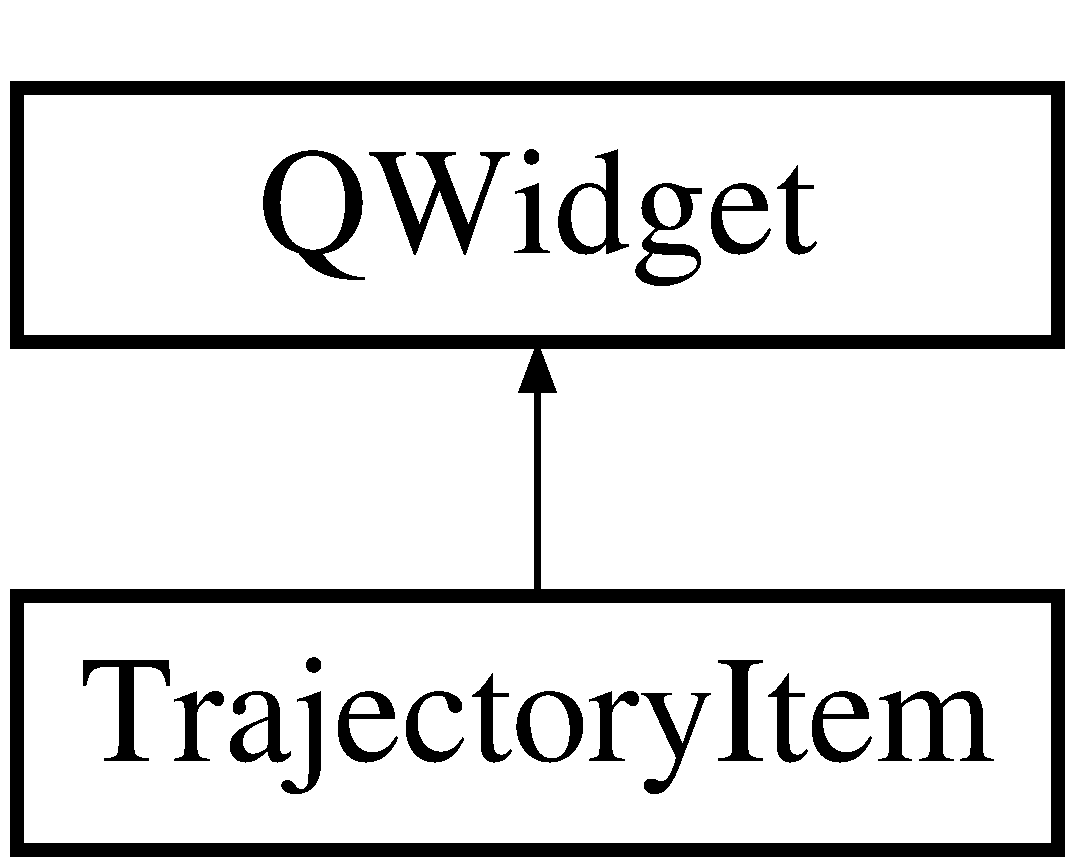
\includegraphics[height=2.000000cm]{classTrajectoryItem}
\end{center}
\end{figure}
\subsection*{Public Member Functions}
\begin{DoxyCompactItemize}
\item 
\hyperlink{classTrajectoryItem_aec384c56b69d666cf6f02b7c4d3fc63a}{Trajectory\+Item} (int64\+\_\+t timestamp, unsigned long time\+Position, unsigned long total\+Time, unsigned long frame\+Number, unsigned long frame\+Count, \hyperlink{structSelection}{Selection} position, Q\+Widget $\ast$parent, bool display\+Time=false)
\item 
\hyperlink{classTrajectoryItem_a8affd9424072ada1f3058e5021c3b54f}{$\sim$\+Trajectory\+Item} ()
\item 
int64\+\_\+t \hyperlink{classTrajectoryItem_aa832c4a147087c2c5c33507f9bde20dd}{get\+\_\+timestamp} () const 
\item 
void \hyperlink{classTrajectoryItem_aac11cf95cd7d71fb567c7b7bbecea402}{display\+\_\+time} ()
\item 
void \hyperlink{classTrajectoryItem_a4f2b20acbd5e0f017ffbfc92d81d526a}{display\+\_\+frame\+\_\+num} ()
\end{DoxyCompactItemize}
\subsection*{Protected Member Functions}
\begin{DoxyCompactItemize}
\item 
bool \hyperlink{classTrajectoryItem_ade2ba7e092a0790fe29517071f257f35}{event\+Filter} (Q\+Object $\ast$object, Q\+Event $\ast$event)
\end{DoxyCompactItemize}


\subsection{Detailed Description}


Definition at line 20 of file trajectoryitem.\+h.



\subsection{Constructor \& Destructor Documentation}
\hypertarget{classTrajectoryItem_aec384c56b69d666cf6f02b7c4d3fc63a}{}\index{Trajectory\+Item@{Trajectory\+Item}!Trajectory\+Item@{Trajectory\+Item}}
\index{Trajectory\+Item@{Trajectory\+Item}!Trajectory\+Item@{Trajectory\+Item}}
\subsubsection[{Trajectory\+Item}]{\setlength{\rightskip}{0pt plus 5cm}Trajectory\+Item\+::\+Trajectory\+Item (
\begin{DoxyParamCaption}
\item[{int64\+\_\+t}]{timestamp, }
\item[{unsigned long}]{time\+Position, }
\item[{unsigned long}]{total\+Time, }
\item[{unsigned long}]{frame\+Number, }
\item[{unsigned long}]{frame\+Count, }
\item[{{\bf Selection}}]{position, }
\item[{Q\+Widget $\ast$}]{parent, }
\item[{bool}]{display\+Time = {\ttfamily false}}
\end{DoxyParamCaption}
)}\label{classTrajectoryItem_aec384c56b69d666cf6f02b7c4d3fc63a}
Constructor 
\begin{DoxyParams}{Parameters}
{\em timestamp} & Timestamp \\
\hline
{\em time\+Position} & Time position \\
\hline
{\em total\+Time} & Total video time \\
\hline
{\em frame\+Number} & Fram number \\
\hline
{\em frame\+Count} & Number of frames in the video \\
\hline
{\em parent} & Parent widget \\
\hline
{\em display\+Time} & True -\/ display time. False -\/ display frame number \\
\hline
\end{DoxyParams}


Definition at line 12 of file trajectoryitem.\+cpp.

\hypertarget{classTrajectoryItem_a8affd9424072ada1f3058e5021c3b54f}{}\index{Trajectory\+Item@{Trajectory\+Item}!````~Trajectory\+Item@{$\sim$\+Trajectory\+Item}}
\index{````~Trajectory\+Item@{$\sim$\+Trajectory\+Item}!Trajectory\+Item@{Trajectory\+Item}}
\subsubsection[{$\sim$\+Trajectory\+Item}]{\setlength{\rightskip}{0pt plus 5cm}Trajectory\+Item\+::$\sim$\+Trajectory\+Item (
\begin{DoxyParamCaption}
{}
\end{DoxyParamCaption}
)}\label{classTrajectoryItem_a8affd9424072ada1f3058e5021c3b54f}
Destructor 

Definition at line 90 of file trajectoryitem.\+cpp.



\subsection{Member Function Documentation}
\hypertarget{classTrajectoryItem_a4f2b20acbd5e0f017ffbfc92d81d526a}{}\index{Trajectory\+Item@{Trajectory\+Item}!display\+\_\+frame\+\_\+num@{display\+\_\+frame\+\_\+num}}
\index{display\+\_\+frame\+\_\+num@{display\+\_\+frame\+\_\+num}!Trajectory\+Item@{Trajectory\+Item}}
\subsubsection[{display\+\_\+frame\+\_\+num}]{\setlength{\rightskip}{0pt plus 5cm}void Trajectory\+Item\+::display\+\_\+frame\+\_\+num (
\begin{DoxyParamCaption}
{}
\end{DoxyParamCaption}
)}\label{classTrajectoryItem_a4f2b20acbd5e0f017ffbfc92d81d526a}
Displays values as frame numbers. 

Definition at line 106 of file trajectoryitem.\+cpp.

\hypertarget{classTrajectoryItem_aac11cf95cd7d71fb567c7b7bbecea402}{}\index{Trajectory\+Item@{Trajectory\+Item}!display\+\_\+time@{display\+\_\+time}}
\index{display\+\_\+time@{display\+\_\+time}!Trajectory\+Item@{Trajectory\+Item}}
\subsubsection[{display\+\_\+time}]{\setlength{\rightskip}{0pt plus 5cm}void Trajectory\+Item\+::display\+\_\+time (
\begin{DoxyParamCaption}
{}
\end{DoxyParamCaption}
)}\label{classTrajectoryItem_aac11cf95cd7d71fb567c7b7bbecea402}
Displays values as time positions. 

Definition at line 100 of file trajectoryitem.\+cpp.

\hypertarget{classTrajectoryItem_ade2ba7e092a0790fe29517071f257f35}{}\index{Trajectory\+Item@{Trajectory\+Item}!event\+Filter@{event\+Filter}}
\index{event\+Filter@{event\+Filter}!Trajectory\+Item@{Trajectory\+Item}}
\subsubsection[{event\+Filter}]{\setlength{\rightskip}{0pt plus 5cm}bool Trajectory\+Item\+::event\+Filter (
\begin{DoxyParamCaption}
\item[{Q\+Object $\ast$}]{object, }
\item[{Q\+Event $\ast$}]{event}
\end{DoxyParamCaption}
)\hspace{0.3cm}{\ttfamily [protected]}}\label{classTrajectoryItem_ade2ba7e092a0790fe29517071f257f35}
Filters Enter and Leave events for item highlighting when hovering 
\begin{DoxyParams}{Parameters}
{\em object} & Object of the event \\
\hline
{\em event} & Event \\
\hline
\end{DoxyParams}
\begin{DoxyReturn}{Returns}
False -\/ propagate event further. True -\/ do not propagate. 
\end{DoxyReturn}


Definition at line 72 of file trajectoryitem.\+cpp.

\hypertarget{classTrajectoryItem_aa832c4a147087c2c5c33507f9bde20dd}{}\index{Trajectory\+Item@{Trajectory\+Item}!get\+\_\+timestamp@{get\+\_\+timestamp}}
\index{get\+\_\+timestamp@{get\+\_\+timestamp}!Trajectory\+Item@{Trajectory\+Item}}
\subsubsection[{get\+\_\+timestamp}]{\setlength{\rightskip}{0pt plus 5cm}int64\+\_\+t Trajectory\+Item\+::get\+\_\+timestamp (
\begin{DoxyParamCaption}
{}
\end{DoxyParamCaption}
) const}\label{classTrajectoryItem_aa832c4a147087c2c5c33507f9bde20dd}
Returns timestamp. \begin{DoxyReturn}{Returns}
timestamp 
\end{DoxyReturn}


Definition at line 95 of file trajectoryitem.\+cpp.



The documentation for this class was generated from the following files\+:\begin{DoxyCompactItemize}
\item 
headers/\hyperlink{trajectoryitem_8h}{trajectoryitem.\+h}\item 
sources/\hyperlink{trajectoryitem_8cpp}{trajectoryitem.\+cpp}\end{DoxyCompactItemize}

\hypertarget{structTrajectorySection}{}\section{Trajectory\+Section Struct Reference}
\label{structTrajectorySection}\index{Trajectory\+Section@{Trajectory\+Section}}


{\ttfamily \#include $<$trackedobject.\+h$>$}

\subsection*{Public Member Functions}
\begin{DoxyCompactItemize}
\item 
{\footnotesize template$<$class Archive $>$ }\\void \hyperlink{structTrajectorySection_aa8a375caa7bc865589e494b070411a73}{serialize} (Archive \&archive)
\item 
\hyperlink{structTrajectorySection_a8514a1d0f2d4416f76a605a9b22bdd56}{Trajectory\+Section} ()
\item 
\hyperlink{structTrajectorySection_ae8bfb8a667d501c6423c2cb24bf40412}{Trajectory\+Section} (\hyperlink{structSelection}{Selection} initial\+Position, int64\+\_\+t initial\+Timestamp, unsigned long initial\+Time\+Position, unsigned long initial\+Frame\+Number)
\end{DoxyCompactItemize}
\subsection*{Public Attributes}
\begin{DoxyCompactItemize}
\item 
\hypertarget{structTrajectorySection_ad07d60f8a921f5c77b19b8c6c8b3dd36}{}\hyperlink{structSelection}{Selection} {\bfseries initial\+Position}\label{structTrajectorySection_ad07d60f8a921f5c77b19b8c6c8b3dd36}

\item 
\hypertarget{structTrajectorySection_a2334c0ba542c815d0a22cd468eb2334e}{}int64\+\_\+t {\bfseries initial\+Timestamp}\label{structTrajectorySection_a2334c0ba542c815d0a22cd468eb2334e}

\item 
\hypertarget{structTrajectorySection_adeaa69f62cab9464d79df0c1cac2dd6e}{}unsigned long {\bfseries initial\+Time\+Position}\label{structTrajectorySection_adeaa69f62cab9464d79df0c1cac2dd6e}

\item 
\hypertarget{structTrajectorySection_a364acaf98a97000611bdcbb3deb3030f}{}unsigned long {\bfseries initial\+Frame\+Number}\label{structTrajectorySection_a364acaf98a97000611bdcbb3deb3030f}

\item 
\hypertarget{structTrajectorySection_a5c64979fad2b666bb13ae305a560ff54}{}\hyperlink{classTrackingAlgorithm}{Tracking\+Algorithm} $\ast$ {\bfseries tracking\+Algorithm}\label{structTrajectorySection_a5c64979fad2b666bb13ae305a560ff54}

\end{DoxyCompactItemize}


\subsection{Detailed Description}
\#define V\+I\+D\+E\+O\+T\+R\+A\+C\+K\+I\+N\+G\+\_\+\+E\+N\+D\+\_\+\+O\+F\+\_\+\+V\+I\+D\+E\+O -\/1 \#define V\+I\+D\+E\+O\+T\+R\+A\+C\+K\+I\+N\+G\+\_\+\+A\+L\+L\+\_\+\+P\+R\+O\+C\+E\+S\+S\+E\+D -\/1 \#define V\+I\+D\+E\+O\+T\+R\+A\+C\+K\+I\+N\+G\+\_\+\+N\+O\+T\+H\+I\+N\+G\+\_\+\+P\+R\+O\+C\+E\+S\+S\+E\+D -\/2 \#define V\+I\+D\+E\+O\+T\+R\+A\+C\+K\+I\+N\+G\+\_\+\+N\+O\+\_\+\+P\+R\+E\+V\+I\+O\+U\+S\+\_\+\+T\+I\+M\+E\+S\+T\+A\+M\+P -\/3 // In case other function than \hyperlink{classVideoTracker_a23bd7731d886bd23007303246f1fb971}{Video\+Tracker\+::get\+\_\+next\+\_\+frame()} is used 

Definition at line 34 of file trackedobject.\+h.



\subsection{Constructor \& Destructor Documentation}
\hypertarget{structTrajectorySection_a8514a1d0f2d4416f76a605a9b22bdd56}{}\index{Trajectory\+Section@{Trajectory\+Section}!Trajectory\+Section@{Trajectory\+Section}}
\index{Trajectory\+Section@{Trajectory\+Section}!Trajectory\+Section@{Trajectory\+Section}}
\subsubsection[{Trajectory\+Section}]{\setlength{\rightskip}{0pt plus 5cm}Trajectory\+Section\+::\+Trajectory\+Section (
\begin{DoxyParamCaption}
{}
\end{DoxyParamCaption}
)\hspace{0.3cm}{\ttfamily [inline]}}\label{structTrajectorySection_a8514a1d0f2d4416f76a605a9b22bdd56}
Constructor 

Definition at line 49 of file trackedobject.\+h.

\hypertarget{structTrajectorySection_ae8bfb8a667d501c6423c2cb24bf40412}{}\index{Trajectory\+Section@{Trajectory\+Section}!Trajectory\+Section@{Trajectory\+Section}}
\index{Trajectory\+Section@{Trajectory\+Section}!Trajectory\+Section@{Trajectory\+Section}}
\subsubsection[{Trajectory\+Section}]{\setlength{\rightskip}{0pt plus 5cm}Trajectory\+Section\+::\+Trajectory\+Section (
\begin{DoxyParamCaption}
\item[{{\bf Selection}}]{initial\+Position, }
\item[{int64\+\_\+t}]{initial\+Timestamp, }
\item[{unsigned long}]{initial\+Time\+Position, }
\item[{unsigned long}]{initial\+Frame\+Number}
\end{DoxyParamCaption}
)\hspace{0.3cm}{\ttfamily [inline]}}\label{structTrajectorySection_ae8bfb8a667d501c6423c2cb24bf40412}
Constructor 
\begin{DoxyParams}{Parameters}
{\em initial\+Position} & Initial object position \\
\hline
{\em initial\+Timestamp} & \\
\hline
{\em initial\+Time\+Position} & \\
\hline
{\em initial\+Frame\+Number} & \\
\hline
\end{DoxyParams}


Definition at line 61 of file trackedobject.\+h.



\subsection{Member Function Documentation}
\hypertarget{structTrajectorySection_aa8a375caa7bc865589e494b070411a73}{}\index{Trajectory\+Section@{Trajectory\+Section}!serialize@{serialize}}
\index{serialize@{serialize}!Trajectory\+Section@{Trajectory\+Section}}
\subsubsection[{serialize}]{\setlength{\rightskip}{0pt plus 5cm}template$<$class Archive $>$ void Trajectory\+Section\+::serialize (
\begin{DoxyParamCaption}
\item[{Archive \&}]{archive}
\end{DoxyParamCaption}
)\hspace{0.3cm}{\ttfamily [inline]}}\label{structTrajectorySection_aa8a375caa7bc865589e494b070411a73}
C\+E\+R\+E\+A\+L serialization 

Definition at line 40 of file trackedobject.\+h.



The documentation for this struct was generated from the following file\+:\begin{DoxyCompactItemize}
\item 
headers/\hyperlink{trackedobject_8h}{trackedobject.\+h}\end{DoxyCompactItemize}

\hypertarget{structUserCanceledException}{}\section{User\+Canceled\+Exception Struct Reference}
\label{structUserCanceledException}\index{User\+Canceled\+Exception@{User\+Canceled\+Exception}}
Inheritance diagram for User\+Canceled\+Exception\+:\begin{figure}[H]
\begin{center}
\leavevmode
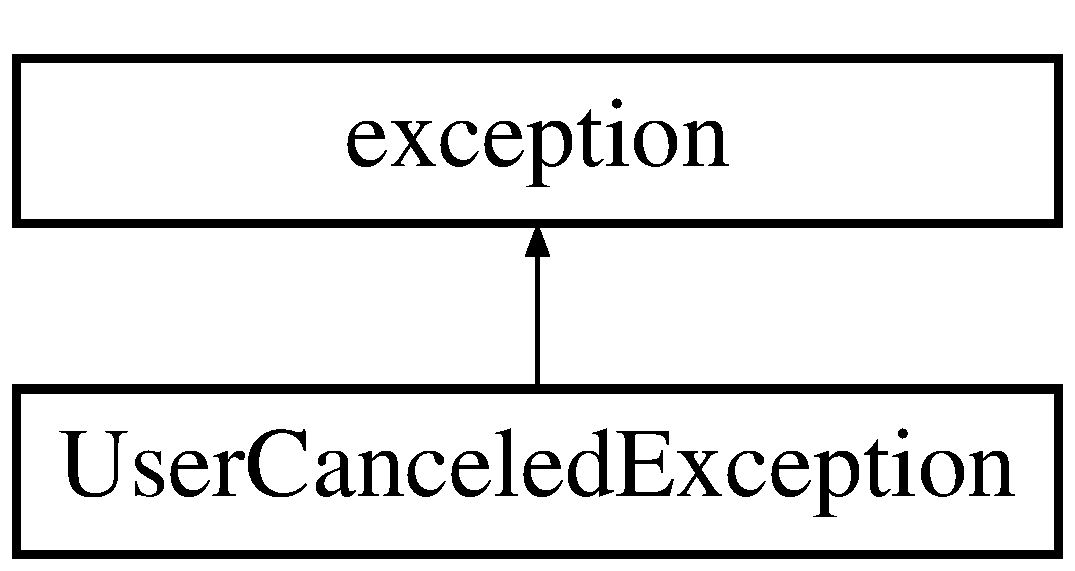
\includegraphics[height=2.000000cm]{structUserCanceledException}
\end{center}
\end{figure}


\subsection{Detailed Description}


Definition at line 31 of file videotracker.\+h.



The documentation for this struct was generated from the following file\+:\begin{DoxyCompactItemize}
\item 
headers/\hyperlink{videotracker_8h}{videotracker.\+h}\end{DoxyCompactItemize}

\hypertarget{structUserCanceledOpeningException}{}\section{User\+Canceled\+Opening\+Exception Struct Reference}
\label{structUserCanceledOpeningException}\index{User\+Canceled\+Opening\+Exception@{User\+Canceled\+Opening\+Exception}}
Inheritance diagram for User\+Canceled\+Opening\+Exception\+:\begin{figure}[H]
\begin{center}
\leavevmode
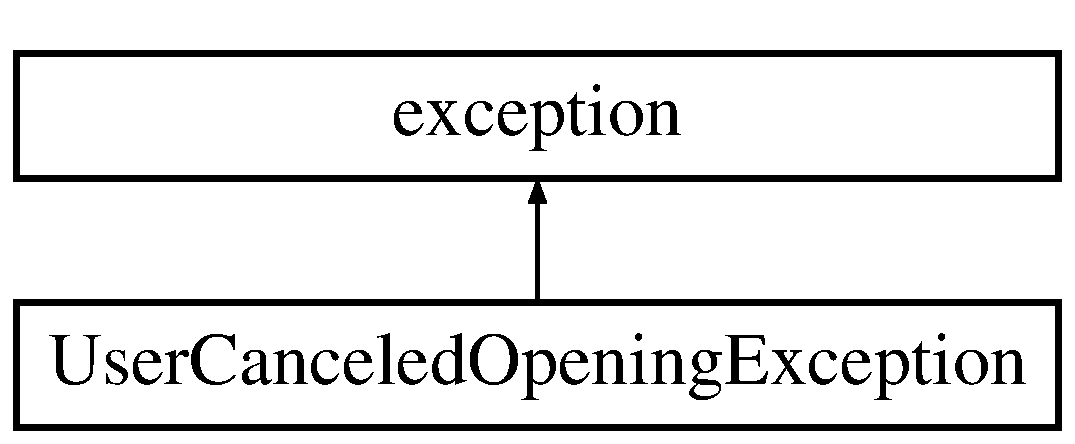
\includegraphics[height=2.000000cm]{structUserCanceledOpeningException}
\end{center}
\end{figure}


\subsection{Detailed Description}


Definition at line 40 of file ffmpegplayer.\+h.



The documentation for this struct was generated from the following file\+:\begin{DoxyCompactItemize}
\item 
headers/\hyperlink{ffmpegplayer_8h}{ffmpegplayer.\+h}\end{DoxyCompactItemize}

\hypertarget{classVideoFrame}{}\section{Video\+Frame Class Reference}
\label{classVideoFrame}\index{Video\+Frame@{Video\+Frame}}
\subsection*{Public Member Functions}
\begin{DoxyCompactItemize}
\item 
\hyperlink{classVideoFrame_ae66f6b32cc93690f42ef8e2d35c6f435}{Video\+Frame} ()
\item 
\hyperlink{classVideoFrame_af5d39a4dcb1e62a1e706b940712d1205}{Video\+Frame} (const \hyperlink{classVideoFrame}{Video\+Frame} \&obj)
\item 
\hyperlink{classVideoFrame_afe4186defd8bbe6613ee5fb105a4f72d}{Video\+Frame} (unsigned int width, unsigned int height)
\item 
\hyperlink{classVideoFrame_af3b566c39ee5878c602581cb1f196675}{$\sim$\+Video\+Frame} ()
\item 
bool \hyperlink{classVideoFrame_a3e5610d8ab84404681fd803b18a158bb}{set\+\_\+frame} (A\+V\+Frame const $\ast$new\+Frame)
\item 
\hypertarget{classVideoFrame_a037a6f6e039413290206427d6fa2c25b}{}unsigned long {\bfseries get\+\_\+time\+\_\+position} () const \label{classVideoFrame_a037a6f6e039413290206427d6fa2c25b}

\item 
int64\+\_\+t \hyperlink{classVideoFrame_a9aa709fcbef2d392cb2a2493af189e91}{get\+\_\+timestamp} () const 
\item 
unsigned long \hyperlink{classVideoFrame_ae090e27da560e3a56dc1ca684e382816}{get\+\_\+frame\+\_\+number} () const 
\item 
unsigned int \hyperlink{classVideoFrame_a4b9af98d459fa34fea270d19768e3f86}{get\+\_\+width} () const 
\item 
unsigned int \hyperlink{classVideoFrame_a20816b24fbb4df819db961bb1b04546f}{get\+\_\+height} () const 
\item 
void \hyperlink{classVideoFrame_a83a8984ee14793bb57b07b409d7b36da}{set\+\_\+size} (unsigned int new\+Width, unsigned int new\+Height)
\item 
void \hyperlink{classVideoFrame_a514a598a06ecb3451192ea3946ab82fc}{set\+\_\+timestamp} (int64\+\_\+t new\+Timestamp)
\item 
void \hyperlink{classVideoFrame_aafed4e7076d4c494e8cb8a75fb158281}{set\+\_\+time\+\_\+position} (unsigned long new\+Time\+Position)
\item 
void \hyperlink{classVideoFrame_a80c39331c68ae3ba658ec6cf9a7b088d}{set\+\_\+frame\+\_\+number} (unsigned long new\+Frame\+Number)
\item 
A\+V\+Frame const $\ast$ \hyperlink{classVideoFrame_ab6c2c0442a4f7bea1193ccf95e5dec6f}{get\+\_\+av\+\_\+frame} ()
\item 
cv\+::\+Mat const $\ast$ \hyperlink{classVideoFrame_ae910256ad8a16261eb676e0f4f93183e}{get\+\_\+mat\+\_\+frame} () const 
\item 
bool \hyperlink{classVideoFrame_a61f14009edeb2d8b1104f4952c23b2d4}{A\+V\+Frame2\+Mat} (A\+V\+Frame const $\ast$src, cv\+::\+Mat $\ast$dst\+Mat) const 
\item 
bool \hyperlink{classVideoFrame_a78b9ebc82b2d22d040895c21452729cc}{Mat2\+A\+V\+Frame} (cv\+::\+Mat const \&src, A\+V\+Frame $\ast$dst\+A\+V\+Frame, const int dst\+Format) const 
\end{DoxyCompactItemize}
\subsection*{Public Attributes}
\begin{DoxyCompactItemize}
\item 
\hypertarget{classVideoFrame_abc5f6e851190c1b76e22cd0e7ed38505}{}cv\+::\+Mat $\ast$ {\bfseries mat\+Frame}\label{classVideoFrame_abc5f6e851190c1b76e22cd0e7ed38505}

\end{DoxyCompactItemize}


\subsection{Detailed Description}


Definition at line 24 of file videoframe.\+h.



\subsection{Constructor \& Destructor Documentation}
\hypertarget{classVideoFrame_ae66f6b32cc93690f42ef8e2d35c6f435}{}\index{Video\+Frame@{Video\+Frame}!Video\+Frame@{Video\+Frame}}
\index{Video\+Frame@{Video\+Frame}!Video\+Frame@{Video\+Frame}}
\subsubsection[{Video\+Frame}]{\setlength{\rightskip}{0pt plus 5cm}Video\+Frame\+::\+Video\+Frame (
\begin{DoxyParamCaption}
{}
\end{DoxyParamCaption}
)}\label{classVideoFrame_ae66f6b32cc93690f42ef8e2d35c6f435}
Constructor 

Definition at line 11 of file videoframe.\+cpp.

\hypertarget{classVideoFrame_af5d39a4dcb1e62a1e706b940712d1205}{}\index{Video\+Frame@{Video\+Frame}!Video\+Frame@{Video\+Frame}}
\index{Video\+Frame@{Video\+Frame}!Video\+Frame@{Video\+Frame}}
\subsubsection[{Video\+Frame}]{\setlength{\rightskip}{0pt plus 5cm}Video\+Frame\+::\+Video\+Frame (
\begin{DoxyParamCaption}
\item[{const {\bf Video\+Frame} \&}]{obj}
\end{DoxyParamCaption}
)}\label{classVideoFrame_af5d39a4dcb1e62a1e706b940712d1205}
Copy constructor 
\begin{DoxyParams}{Parameters}
{\em obj} & Original \\
\hline
\end{DoxyParams}


Definition at line 31 of file videoframe.\+cpp.

\hypertarget{classVideoFrame_afe4186defd8bbe6613ee5fb105a4f72d}{}\index{Video\+Frame@{Video\+Frame}!Video\+Frame@{Video\+Frame}}
\index{Video\+Frame@{Video\+Frame}!Video\+Frame@{Video\+Frame}}
\subsubsection[{Video\+Frame}]{\setlength{\rightskip}{0pt plus 5cm}Video\+Frame\+::\+Video\+Frame (
\begin{DoxyParamCaption}
\item[{unsigned int}]{width, }
\item[{unsigned int}]{height}
\end{DoxyParamCaption}
)}\label{classVideoFrame_afe4186defd8bbe6613ee5fb105a4f72d}
Constructor 
\begin{DoxyParams}{Parameters}
{\em width} & Frame width \\
\hline
{\em height} & Frame height \\
\hline
\end{DoxyParams}


Definition at line 20 of file videoframe.\+cpp.

\hypertarget{classVideoFrame_af3b566c39ee5878c602581cb1f196675}{}\index{Video\+Frame@{Video\+Frame}!````~Video\+Frame@{$\sim$\+Video\+Frame}}
\index{````~Video\+Frame@{$\sim$\+Video\+Frame}!Video\+Frame@{Video\+Frame}}
\subsubsection[{$\sim$\+Video\+Frame}]{\setlength{\rightskip}{0pt plus 5cm}Video\+Frame\+::$\sim$\+Video\+Frame (
\begin{DoxyParamCaption}
{}
\end{DoxyParamCaption}
)}\label{classVideoFrame_af3b566c39ee5878c602581cb1f196675}
Destructor 

Definition at line 47 of file videoframe.\+cpp.



\subsection{Member Function Documentation}
\hypertarget{classVideoFrame_a61f14009edeb2d8b1104f4952c23b2d4}{}\index{Video\+Frame@{Video\+Frame}!A\+V\+Frame2\+Mat@{A\+V\+Frame2\+Mat}}
\index{A\+V\+Frame2\+Mat@{A\+V\+Frame2\+Mat}!Video\+Frame@{Video\+Frame}}
\subsubsection[{A\+V\+Frame2\+Mat}]{\setlength{\rightskip}{0pt plus 5cm}bool Video\+Frame\+::\+A\+V\+Frame2\+Mat (
\begin{DoxyParamCaption}
\item[{A\+V\+Frame const $\ast$}]{src, }
\item[{cv\+::\+Mat $\ast$}]{dst\+Mat}
\end{DoxyParamCaption}
) const}\label{classVideoFrame_a61f14009edeb2d8b1104f4952c23b2d4}
Converts A\+V\+Frame to cv\+::\+Mat. 
\begin{DoxyParams}{Parameters}
{\em src} & Source A\+V\+Frame \\
\hline
{\em dst\+Mat} & Destination cv\+::\+Mat; It mus be allocated before using this function. \\
\hline
\end{DoxyParams}
\begin{DoxyReturn}{Returns}
True if successful 
\end{DoxyReturn}


Definition at line 176 of file videoframe.\+cpp.

\hypertarget{classVideoFrame_ab6c2c0442a4f7bea1193ccf95e5dec6f}{}\index{Video\+Frame@{Video\+Frame}!get\+\_\+av\+\_\+frame@{get\+\_\+av\+\_\+frame}}
\index{get\+\_\+av\+\_\+frame@{get\+\_\+av\+\_\+frame}!Video\+Frame@{Video\+Frame}}
\subsubsection[{get\+\_\+av\+\_\+frame}]{\setlength{\rightskip}{0pt plus 5cm}A\+V\+Frame const $\ast$ Video\+Frame\+::get\+\_\+av\+\_\+frame (
\begin{DoxyParamCaption}
{}
\end{DoxyParamCaption}
)}\label{classVideoFrame_ab6c2c0442a4f7bea1193ccf95e5dec6f}
Returns the frame in A\+V\+Frame. \begin{DoxyReturn}{Returns}
Frame 
\end{DoxyReturn}


Definition at line 130 of file videoframe.\+cpp.

\hypertarget{classVideoFrame_ae090e27da560e3a56dc1ca684e382816}{}\index{Video\+Frame@{Video\+Frame}!get\+\_\+frame\+\_\+number@{get\+\_\+frame\+\_\+number}}
\index{get\+\_\+frame\+\_\+number@{get\+\_\+frame\+\_\+number}!Video\+Frame@{Video\+Frame}}
\subsubsection[{get\+\_\+frame\+\_\+number}]{\setlength{\rightskip}{0pt plus 5cm}unsigned long Video\+Frame\+::get\+\_\+frame\+\_\+number (
\begin{DoxyParamCaption}
{}
\end{DoxyParamCaption}
) const}\label{classVideoFrame_ae090e27da560e3a56dc1ca684e382816}
Returns frame number (index). \begin{DoxyReturn}{Returns}
Frame number 
\end{DoxyReturn}


Definition at line 87 of file videoframe.\+cpp.

\hypertarget{classVideoFrame_a20816b24fbb4df819db961bb1b04546f}{}\index{Video\+Frame@{Video\+Frame}!get\+\_\+height@{get\+\_\+height}}
\index{get\+\_\+height@{get\+\_\+height}!Video\+Frame@{Video\+Frame}}
\subsubsection[{get\+\_\+height}]{\setlength{\rightskip}{0pt plus 5cm}unsigned int Video\+Frame\+::get\+\_\+height (
\begin{DoxyParamCaption}
{}
\end{DoxyParamCaption}
) const}\label{classVideoFrame_a20816b24fbb4df819db961bb1b04546f}
Returns height of the frame. \begin{DoxyReturn}{Returns}
Frame height 
\end{DoxyReturn}


Definition at line 97 of file videoframe.\+cpp.

\hypertarget{classVideoFrame_ae910256ad8a16261eb676e0f4f93183e}{}\index{Video\+Frame@{Video\+Frame}!get\+\_\+mat\+\_\+frame@{get\+\_\+mat\+\_\+frame}}
\index{get\+\_\+mat\+\_\+frame@{get\+\_\+mat\+\_\+frame}!Video\+Frame@{Video\+Frame}}
\subsubsection[{get\+\_\+mat\+\_\+frame}]{\setlength{\rightskip}{0pt plus 5cm}cv\+::\+Mat const $\ast$ Video\+Frame\+::get\+\_\+mat\+\_\+frame (
\begin{DoxyParamCaption}
{}
\end{DoxyParamCaption}
) const}\label{classVideoFrame_ae910256ad8a16261eb676e0f4f93183e}
Returns the frame in cv\+::\+Mat. \begin{DoxyReturn}{Returns}
Frame 
\end{DoxyReturn}


Definition at line 170 of file videoframe.\+cpp.

\hypertarget{classVideoFrame_a9aa709fcbef2d392cb2a2493af189e91}{}\index{Video\+Frame@{Video\+Frame}!get\+\_\+timestamp@{get\+\_\+timestamp}}
\index{get\+\_\+timestamp@{get\+\_\+timestamp}!Video\+Frame@{Video\+Frame}}
\subsubsection[{get\+\_\+timestamp}]{\setlength{\rightskip}{0pt plus 5cm}int64\+\_\+t Video\+Frame\+::get\+\_\+timestamp (
\begin{DoxyParamCaption}
{}
\end{DoxyParamCaption}
) const}\label{classVideoFrame_a9aa709fcbef2d392cb2a2493af189e91}
Returns frame timestamp. \begin{DoxyReturn}{Returns}
Frame timestamp 
\end{DoxyReturn}


Definition at line 82 of file videoframe.\+cpp.

\hypertarget{classVideoFrame_a4b9af98d459fa34fea270d19768e3f86}{}\index{Video\+Frame@{Video\+Frame}!get\+\_\+width@{get\+\_\+width}}
\index{get\+\_\+width@{get\+\_\+width}!Video\+Frame@{Video\+Frame}}
\subsubsection[{get\+\_\+width}]{\setlength{\rightskip}{0pt plus 5cm}unsigned int Video\+Frame\+::get\+\_\+width (
\begin{DoxyParamCaption}
{}
\end{DoxyParamCaption}
) const}\label{classVideoFrame_a4b9af98d459fa34fea270d19768e3f86}
Returns width of the frame. \begin{DoxyReturn}{Returns}
Frame width 
\end{DoxyReturn}


Definition at line 92 of file videoframe.\+cpp.

\hypertarget{classVideoFrame_a78b9ebc82b2d22d040895c21452729cc}{}\index{Video\+Frame@{Video\+Frame}!Mat2\+A\+V\+Frame@{Mat2\+A\+V\+Frame}}
\index{Mat2\+A\+V\+Frame@{Mat2\+A\+V\+Frame}!Video\+Frame@{Video\+Frame}}
\subsubsection[{Mat2\+A\+V\+Frame}]{\setlength{\rightskip}{0pt plus 5cm}bool Video\+Frame\+::\+Mat2\+A\+V\+Frame (
\begin{DoxyParamCaption}
\item[{cv\+::\+Mat const \&}]{src, }
\item[{A\+V\+Frame $\ast$}]{dst\+A\+V\+Frame, }
\item[{const int}]{dst\+Format}
\end{DoxyParamCaption}
) const}\label{classVideoFrame_a78b9ebc82b2d22d040895c21452729cc}
Converts cv\+::\+Mat to A\+V\+Frame. 
\begin{DoxyParams}{Parameters}
{\em src} & Source cv\+::at \\
\hline
{\em dst\+A\+V\+Frame} & Destination A\+V\+Frame \\
\hline
{\em dst\+Format} & Destination Pixel\+Format; it must be allocated before, but must not have allocated buffer (is allocated inside of this function). The buffer needs to be later freed manually. \\
\hline
\end{DoxyParams}
\begin{DoxyReturn}{Returns}
True if successful 
\end{DoxyReturn}


Definition at line 213 of file videoframe.\+cpp.

\hypertarget{classVideoFrame_a3e5610d8ab84404681fd803b18a158bb}{}\index{Video\+Frame@{Video\+Frame}!set\+\_\+frame@{set\+\_\+frame}}
\index{set\+\_\+frame@{set\+\_\+frame}!Video\+Frame@{Video\+Frame}}
\subsubsection[{set\+\_\+frame}]{\setlength{\rightskip}{0pt plus 5cm}bool Video\+Frame\+::set\+\_\+frame (
\begin{DoxyParamCaption}
\item[{A\+V\+Frame const $\ast$}]{new\+Frame}
\end{DoxyParamCaption}
)}\label{classVideoFrame_a3e5610d8ab84404681fd803b18a158bb}
Sets a new frame 
\begin{DoxyParams}{Parameters}
{\em new\+Frame} & New frame data \\
\hline
\end{DoxyParams}
\begin{DoxyReturn}{Returns}
True if successful 
\end{DoxyReturn}


Definition at line 62 of file videoframe.\+cpp.

\hypertarget{classVideoFrame_a80c39331c68ae3ba658ec6cf9a7b088d}{}\index{Video\+Frame@{Video\+Frame}!set\+\_\+frame\+\_\+number@{set\+\_\+frame\+\_\+number}}
\index{set\+\_\+frame\+\_\+number@{set\+\_\+frame\+\_\+number}!Video\+Frame@{Video\+Frame}}
\subsubsection[{set\+\_\+frame\+\_\+number}]{\setlength{\rightskip}{0pt plus 5cm}void Video\+Frame\+::set\+\_\+frame\+\_\+number (
\begin{DoxyParamCaption}
\item[{unsigned long}]{new\+Frame\+Number}
\end{DoxyParamCaption}
)}\label{classVideoFrame_a80c39331c68ae3ba658ec6cf9a7b088d}
Sets frame number. 
\begin{DoxyParams}{Parameters}
{\em new\+Frame\+Number} & New frame number \\
\hline
\end{DoxyParams}


Definition at line 125 of file videoframe.\+cpp.

\hypertarget{classVideoFrame_a83a8984ee14793bb57b07b409d7b36da}{}\index{Video\+Frame@{Video\+Frame}!set\+\_\+size@{set\+\_\+size}}
\index{set\+\_\+size@{set\+\_\+size}!Video\+Frame@{Video\+Frame}}
\subsubsection[{set\+\_\+size}]{\setlength{\rightskip}{0pt plus 5cm}void Video\+Frame\+::set\+\_\+size (
\begin{DoxyParamCaption}
\item[{unsigned int}]{new\+Width, }
\item[{unsigned int}]{new\+Height}
\end{DoxyParamCaption}
)}\label{classVideoFrame_a83a8984ee14793bb57b07b409d7b36da}
Sets frame size. 
\begin{DoxyParams}{Parameters}
{\em new\+Width} & New frame width \\
\hline
{\em new\+Height} & New frame height \\
\hline
\end{DoxyParams}


Definition at line 102 of file videoframe.\+cpp.

\hypertarget{classVideoFrame_aafed4e7076d4c494e8cb8a75fb158281}{}\index{Video\+Frame@{Video\+Frame}!set\+\_\+time\+\_\+position@{set\+\_\+time\+\_\+position}}
\index{set\+\_\+time\+\_\+position@{set\+\_\+time\+\_\+position}!Video\+Frame@{Video\+Frame}}
\subsubsection[{set\+\_\+time\+\_\+position}]{\setlength{\rightskip}{0pt plus 5cm}void Video\+Frame\+::set\+\_\+time\+\_\+position (
\begin{DoxyParamCaption}
\item[{unsigned long}]{new\+Time\+Position}
\end{DoxyParamCaption}
)}\label{classVideoFrame_aafed4e7076d4c494e8cb8a75fb158281}
Sets time position. 
\begin{DoxyParams}{Parameters}
{\em new\+Time\+Position} & New time Position \\
\hline
\end{DoxyParams}


Definition at line 120 of file videoframe.\+cpp.

\hypertarget{classVideoFrame_a514a598a06ecb3451192ea3946ab82fc}{}\index{Video\+Frame@{Video\+Frame}!set\+\_\+timestamp@{set\+\_\+timestamp}}
\index{set\+\_\+timestamp@{set\+\_\+timestamp}!Video\+Frame@{Video\+Frame}}
\subsubsection[{set\+\_\+timestamp}]{\setlength{\rightskip}{0pt plus 5cm}void Video\+Frame\+::set\+\_\+timestamp (
\begin{DoxyParamCaption}
\item[{int64\+\_\+t}]{new\+Timestamp}
\end{DoxyParamCaption}
)}\label{classVideoFrame_a514a598a06ecb3451192ea3946ab82fc}
Sets timestamp. 
\begin{DoxyParams}{Parameters}
{\em new\+Timestamp} & New timestamp \\
\hline
\end{DoxyParams}


Definition at line 115 of file videoframe.\+cpp.



The documentation for this class was generated from the following files\+:\begin{DoxyCompactItemize}
\item 
headers/\hyperlink{videoframe_8h}{videoframe.\+h}\item 
sources/\hyperlink{videoframe_8cpp}{videoframe.\+cpp}\end{DoxyCompactItemize}

\hypertarget{classVideoTracker}{}\section{Video\+Tracker Class Reference}
\label{classVideoTracker}\index{Video\+Tracker@{Video\+Tracker}}
\subsection*{Public Member Functions}
\begin{DoxyCompactItemize}
\item 
\hypertarget{classVideoTracker_a829485245ee54ecc195c3069024e615b}{}{\footnotesize template$<$class Archive $>$ }\\void {\bfseries serialize} (Archive \&archive)\label{classVideoTracker_a829485245ee54ecc195c3069024e615b}

\item 
\hyperlink{classVideoTracker_a8a4eb43cf75ecaec34b1b54b99d7e701}{Video\+Tracker} ()
\item 
\hyperlink{classVideoTracker_a83a8ecb8fe646a44aaa1c892e9a69a65}{Video\+Tracker} (std\+::string const \&video\+Addr, Q\+Progress\+Dialog const $\ast$progress\+Dialog)
\item 
\hyperlink{classVideoTracker_ac20788504b98efbae977d3d55459b443}{$\sim$\+Video\+Tracker} ()
\item 
void \hyperlink{classVideoTracker_aef0c8e2fbeaaac3fcd1737c457a4c0ea}{load\+\_\+video} (std\+::string const \&video\+Addr, Q\+Progress\+Dialog const $\ast$progress\+Dialog)
\item 
double \hyperlink{classVideoTracker_a2e429fbc7d3f7c4904bcfab51c8aae25}{get\+\_\+fps} () const 
\item 
unsigned long \hyperlink{classVideoTracker_af5ef823d494e6fdc75b4aedbd8739ba5}{get\+\_\+frame\+\_\+count} () const 
\item 
unsigned long \hyperlink{classVideoTracker_ac442e8d7148366c07b71ec4fc0505e5b}{get\+\_\+total\+\_\+time} () const 
\item 
int64\+\_\+t \hyperlink{classVideoTracker_ac9a2a134bbc59f24defb0d8920e1d79c}{get\+\_\+frame\+\_\+timestamp} () const 
\item 
unsigned long \hyperlink{classVideoTracker_a21c40e168f99bf04abfb071406b060b5}{get\+\_\+time\+\_\+position} () const 
\item 
unsigned long \hyperlink{classVideoTracker_afa5bf7dc2a1a5b90d762ff310dfc89b8}{get\+\_\+frame\+\_\+number} () const 
\item 
unsigned int \hyperlink{classVideoTracker_ab8d3f48ad0615b992ac0f767f206d2af}{get\+\_\+objects\+\_\+count} () const 
\item 
int \hyperlink{classVideoTracker_ac5078e2bfb902a7b24d76bcd570bc8f2}{add\+\_\+object} (const \hyperlink{structCharacteristics}{Characteristics} \&object\+Appearance, const std\+::string \&object\+Name, \hyperlink{structSelection}{Selection} initial\+Position, int64\+\_\+t initial\+Timestamp, unsigned long initial\+Time\+Position, unsigned long initial\+Frame\+Number, bool end\+Timestamp\+Set=false, int64\+\_\+t end\+Timestamp=0, unsigned long end\+Time\+Position=0, unsigned long end\+Frame\+Number=0)
\item 
bool \hyperlink{classVideoTracker_a3edec586640511e2a3e58605cfb7545d}{get\+\_\+frame\+\_\+by\+\_\+time} (Q\+Image \&img\+Frame, Q\+Image \&original\+Img\+Frame, bool include\+Original, int64\+\_\+t time, Q\+Progress\+Dialog $\ast$progress\+Dialog)
\item 
bool \hyperlink{classVideoTracker_a5c146358a49c5c0d7d6e2ff2029b1bfb}{get\+\_\+frame\+\_\+by\+\_\+timestamp} (Q\+Image \&img\+Frame, Q\+Image \&original\+Img\+Frame, bool include\+Original, int64\+\_\+t timestamp, Q\+Progress\+Dialog $\ast$progress\+Dialog)
\item 
bool \hyperlink{classVideoTracker_a6d0260650063aa10284d1645bbbee778}{get\+\_\+frame\+\_\+by\+\_\+number} (Q\+Image \&img\+Frame, Q\+Image \&original\+Img\+Frame, bool include\+Original, unsigned long frame\+Number, Q\+Progress\+Dialog $\ast$progress\+Dialog)
\item 
bool \hyperlink{classVideoTracker_a23bd7731d886bd23007303246f1fb971}{get\+\_\+next\+\_\+frame} (Q\+Image \&img\+Frame, Q\+Image \&original\+Img\+Frame, bool include\+Original, Q\+Progress\+Dialog $\ast$progress\+Dialog)
\item 
bool \hyperlink{classVideoTracker_ab3f64c39d4550baeb2ef0c4020895761}{get\+\_\+previous\+\_\+frame} (Q\+Image \&img\+Frame, Q\+Image \&original\+Img\+Frame, bool include\+Original, Q\+Progress\+Dialog $\ast$progress\+Dialog)
\item 
bool \hyperlink{classVideoTracker_ac1f10ef86abebc2a2b1b78519e34d14d}{get\+\_\+current\+\_\+frame} (Q\+Image \&img\+Frame, Q\+Image \&original\+Img\+Frame, bool include\+Original)
\item 
bool \hyperlink{classVideoTracker_a9cf68ec22757e2c2a9dc7a8f6b71fc6c}{get\+\_\+first\+\_\+frame} (Q\+Image \&img\+Frame, Q\+Image \&original\+Img\+Frame, bool include\+Original, Q\+Progress\+Dialog $\ast$progress\+Dialog)
\item 
void \hyperlink{classVideoTracker_a155ecb70409e4f4e4670cbe7e5e0e0cd}{create\+\_\+output} (std\+::string const \&filename, Q\+Progress\+Dialog \&file\+Progress\+Dialog, Q\+Progress\+Dialog $\ast$tracking\+Progress\+Dialog, std\+::string in\+File\+Extension)
\item 
\hyperlink{structCharacteristics}{Characteristics} \hyperlink{classVideoTracker_a07349e6584efc93fc2fb480fe6a436b8}{get\+\_\+object\+\_\+appearance} (unsigned int object\+I\+D) const 
\item 
std\+::map$<$ int64\+\_\+t, \hyperlink{structTrajectorySection}{Trajectory\+Section} $>$ const \& \hyperlink{classVideoTracker_aa81777a4dd7aca72a994f883a9ae50e5}{get\+\_\+object\+\_\+trajectory\+\_\+sections} (unsigned int object\+I\+D) const 
\item 
std\+::map$<$ int64\+\_\+t, \hyperlink{structTrajectoryEntry}{Trajectory\+Entry} $>$ const \& \hyperlink{classVideoTracker_a1c65db5d8e998ab3525eb492bf04c171}{get\+\_\+object\+\_\+trajectory} (unsigned int object\+I\+D) const 
\item 
bool \hyperlink{classVideoTracker_a2769b71f5bba913e4cecba2823702eda}{change\+\_\+object\+\_\+appearance} (unsigned int object\+I\+D, \hyperlink{structCharacteristics}{Characteristics} const \&new\+Appearance)
\item 
void \hyperlink{classVideoTracker_ab6a9679646906aea8d6d7730b78e0948}{seek\+\_\+first\+\_\+packet} ()
\item 
bool \hyperlink{classVideoTracker_a50e5a543b8e31e121ac58a159f2384b2}{get\+\_\+object\+\_\+end} (unsigned int object\+I\+D, int64\+\_\+t \&timestamp, unsigned long \&time\+Position, unsigned long \&frame\+Number)
\item 
bool \hyperlink{classVideoTracker_abfdad55bb49e7b2c45140d884856c6bc}{change\+\_\+object\+\_\+trajectory\+\_\+section} (unsigned int object\+I\+D, int64\+\_\+t old\+Timestamp, int64\+\_\+t new\+Timestamp, \hyperlink{structSelection}{Selection} position, unsigned long time\+Position, unsigned long frame\+Number)
\item 
bool \hyperlink{classVideoTracker_ad238b49118cb9c288e4543b509e1e6f8}{change\+\_\+object\+\_\+end\+\_\+frame} (unsigned int object\+I\+D, bool set, int64\+\_\+t new\+Timestamp=0, unsigned long time\+Position=0, unsigned long frame\+Number=0)
\item 
bool \hyperlink{classVideoTracker_afef3f2aad3fc3eadc65400eb757d0e47}{delete\+\_\+object\+\_\+trajectory\+\_\+section} (unsigned int object\+I\+D, int64\+\_\+t timestamp)
\item 
bool \hyperlink{classVideoTracker_a67a4e9d0a476dc6bb04047c8fdc94d5b}{set\+\_\+object\+\_\+trajectory\+\_\+section} (unsigned int object\+I\+D, int64\+\_\+t new\+Timestamp, \hyperlink{structSelection}{Selection} position, unsigned long time\+Position, unsigned long frame\+Number)
\item 
std\+::string \hyperlink{classVideoTracker_a9f967e75fa324d4fc17a7875fe2bef1e}{get\+\_\+object\+\_\+name} (unsigned int object\+I\+D)
\item 
std\+::vector$<$ std\+::string $>$ \hyperlink{classVideoTracker_a6a8d40056c7a309292eb627d84576d3a}{get\+\_\+all\+\_\+objects\+\_\+names} ()
\item 
void \hyperlink{classVideoTracker_ad37c9432c33014bdb3476b31fe16a4ce}{set\+\_\+object\+\_\+name} (unsigned int object\+I\+D, std\+::string new\+Name)
\item 
void \hyperlink{classVideoTracker_a10a09bf6a8f67c378c3bfa60255a007a}{delete\+\_\+object} (unsigned int object\+I\+D)
\item 
bool \hyperlink{classVideoTracker_a7b6b59eea6ef8210a234726524447d9f}{track\+\_\+object} (unsigned int object\+I\+D, Q\+Progress\+Dialog $\ast$progress\+Dialog)
\item 
void \hyperlink{classVideoTracker_a7400741f360deb50b33bc9b96aef9083}{erase\+\_\+object\+\_\+trajectories\+\_\+to\+\_\+comply} ()
\end{DoxyCompactItemize}


\subsection{Detailed Description}


Definition at line 33 of file videotracker.\+h.



\subsection{Constructor \& Destructor Documentation}
\hypertarget{classVideoTracker_a8a4eb43cf75ecaec34b1b54b99d7e701}{}\index{Video\+Tracker@{Video\+Tracker}!Video\+Tracker@{Video\+Tracker}}
\index{Video\+Tracker@{Video\+Tracker}!Video\+Tracker@{Video\+Tracker}}
\subsubsection[{Video\+Tracker}]{\setlength{\rightskip}{0pt plus 5cm}Video\+Tracker\+::\+Video\+Tracker (
\begin{DoxyParamCaption}
{}
\end{DoxyParamCaption}
)}\label{classVideoTracker_a8a4eb43cf75ecaec34b1b54b99d7e701}
Constructor 

Definition at line 15 of file videotracker.\+cpp.

\hypertarget{classVideoTracker_a83a8ecb8fe646a44aaa1c892e9a69a65}{}\index{Video\+Tracker@{Video\+Tracker}!Video\+Tracker@{Video\+Tracker}}
\index{Video\+Tracker@{Video\+Tracker}!Video\+Tracker@{Video\+Tracker}}
\subsubsection[{Video\+Tracker}]{\setlength{\rightskip}{0pt plus 5cm}Video\+Tracker\+::\+Video\+Tracker (
\begin{DoxyParamCaption}
\item[{std\+::string const \&}]{video\+Addr, }
\item[{Q\+Progress\+Dialog const $\ast$}]{progress\+Dialog}
\end{DoxyParamCaption}
)\hspace{0.3cm}{\ttfamily [explicit]}}\label{classVideoTracker_a83a8ecb8fe646a44aaa1c892e9a69a65}
Constructor 
\begin{DoxyParams}{Parameters}
{\em video\+Addr} & Path to a video file \\
\hline
{\em progress\+Dialog} & Q\+T progress dialog for displaying information about video opening \\
\hline
\end{DoxyParams}


Definition at line 23 of file videotracker.\+cpp.

\hypertarget{classVideoTracker_ac20788504b98efbae977d3d55459b443}{}\index{Video\+Tracker@{Video\+Tracker}!````~Video\+Tracker@{$\sim$\+Video\+Tracker}}
\index{````~Video\+Tracker@{$\sim$\+Video\+Tracker}!Video\+Tracker@{Video\+Tracker}}
\subsubsection[{$\sim$\+Video\+Tracker}]{\setlength{\rightskip}{0pt plus 5cm}Video\+Tracker\+::$\sim$\+Video\+Tracker (
\begin{DoxyParamCaption}
{}
\end{DoxyParamCaption}
)}\label{classVideoTracker_ac20788504b98efbae977d3d55459b443}
Destructor for (\hyperlink{classTrackedObject}{Tracked\+Object} $\ast$object\+: tracked\+Objects) \{ delete object; object = nullptr; \}

Definition at line 37 of file videotracker.\+cpp.



\subsection{Member Function Documentation}
\hypertarget{classVideoTracker_ac5078e2bfb902a7b24d76bcd570bc8f2}{}\index{Video\+Tracker@{Video\+Tracker}!add\+\_\+object@{add\+\_\+object}}
\index{add\+\_\+object@{add\+\_\+object}!Video\+Tracker@{Video\+Tracker}}
\subsubsection[{add\+\_\+object}]{\setlength{\rightskip}{0pt plus 5cm}int Video\+Tracker\+::add\+\_\+object (
\begin{DoxyParamCaption}
\item[{const {\bf Characteristics} \&}]{object\+Appearance, }
\item[{const std\+::string \&}]{object\+Name, }
\item[{{\bf Selection}}]{initial\+Position, }
\item[{int64\+\_\+t}]{initial\+Timestamp, }
\item[{unsigned long}]{initial\+Time\+Position, }
\item[{unsigned long}]{initial\+Frame\+Number, }
\item[{bool}]{end\+Timestamp\+Set = {\ttfamily false}, }
\item[{int64\+\_\+t}]{end\+Timestamp = {\ttfamily 0}, }
\item[{unsigned long}]{end\+Time\+Position = {\ttfamily 0}, }
\item[{unsigned long}]{end\+Frame\+Number = {\ttfamily 0}}
\end{DoxyParamCaption}
)}\label{classVideoTracker_ac5078e2bfb902a7b24d76bcd570bc8f2}
Tracks a new object. 
\begin{DoxyParams}{Parameters}
{\em object\+Appearance} & Object appearance \\
\hline
{\em object\+Name} & Object name \\
\hline
{\em initial\+Position} & Initial object position \\
\hline
{\em initial\+Timestamp} & Initial timestamp \\
\hline
{\em initial\+Time\+Position} & Initial time position \\
\hline
{\em initial\+Frame\+Number} & Initial frame number \\
\hline
{\em end\+Timestamp\+Set} & Is end timestamp set? \\
\hline
{\em end\+Timestamp} & End timestamp \\
\hline
{\em end\+Time\+Position} & End time position \\
\hline
{\em end\+Frame\+Number} & End frame number \\
\hline
\end{DoxyParams}
\begin{DoxyReturn}{Returns}
Object I\+D; First objest has I\+D 1. If frame at initial\+Timestamp is not read, -\/1 is returned; 
\end{DoxyReturn}


Definition at line 67 of file videotracker.\+cpp.

\hypertarget{classVideoTracker_a2769b71f5bba913e4cecba2823702eda}{}\index{Video\+Tracker@{Video\+Tracker}!change\+\_\+object\+\_\+appearance@{change\+\_\+object\+\_\+appearance}}
\index{change\+\_\+object\+\_\+appearance@{change\+\_\+object\+\_\+appearance}!Video\+Tracker@{Video\+Tracker}}
\subsubsection[{change\+\_\+object\+\_\+appearance}]{\setlength{\rightskip}{0pt plus 5cm}bool Video\+Tracker\+::change\+\_\+object\+\_\+appearance (
\begin{DoxyParamCaption}
\item[{unsigned int}]{object\+I\+D, }
\item[{{\bf Characteristics} const \&}]{new\+Appearance}
\end{DoxyParamCaption}
)}\label{classVideoTracker_a2769b71f5bba913e4cecba2823702eda}
Changes appearance of the object. 
\begin{DoxyParams}{Parameters}
{\em object\+I\+D} & Object I\+D \\
\hline
{\em new\+Appearance} & New appearance of the object \\
\hline
\end{DoxyParams}


Definition at line 631 of file videotracker.\+cpp.

\hypertarget{classVideoTracker_ad238b49118cb9c288e4543b509e1e6f8}{}\index{Video\+Tracker@{Video\+Tracker}!change\+\_\+object\+\_\+end\+\_\+frame@{change\+\_\+object\+\_\+end\+\_\+frame}}
\index{change\+\_\+object\+\_\+end\+\_\+frame@{change\+\_\+object\+\_\+end\+\_\+frame}!Video\+Tracker@{Video\+Tracker}}
\subsubsection[{change\+\_\+object\+\_\+end\+\_\+frame}]{\setlength{\rightskip}{0pt plus 5cm}bool Video\+Tracker\+::change\+\_\+object\+\_\+end\+\_\+frame (
\begin{DoxyParamCaption}
\item[{unsigned int}]{object\+I\+D, }
\item[{bool}]{set, }
\item[{int64\+\_\+t}]{new\+Timestamp = {\ttfamily 0}, }
\item[{unsigned long}]{time\+Position = {\ttfamily 0}, }
\item[{unsigned long}]{frame\+Number = {\ttfamily 0}}
\end{DoxyParamCaption}
)}\label{classVideoTracker_ad238b49118cb9c288e4543b509e1e6f8}
Changes the end frame of the object. If set==false, the end frame will be unset and the object will be tracked till the end of the video. new\+Timestamp and time\+Position are valid onlt if set==true. 
\begin{DoxyParams}{Parameters}
{\em object\+I\+D} & Object I\+D \\
\hline
{\em set} & Set / Unset last frame \\
\hline
{\em new\+Timestamp} & Timestamp of the last frame \\
\hline
{\em time\+Position} & Time position of the last frame \\
\hline
{\em frame\+Number} & Frame number of the last frame \\
\hline
\end{DoxyParams}
\begin{DoxyReturn}{Returns}
False if given timestamp is lower than the timestamp of Beginning. 
\end{DoxyReturn}


Definition at line 614 of file videotracker.\+cpp.

\hypertarget{classVideoTracker_abfdad55bb49e7b2c45140d884856c6bc}{}\index{Video\+Tracker@{Video\+Tracker}!change\+\_\+object\+\_\+trajectory\+\_\+section@{change\+\_\+object\+\_\+trajectory\+\_\+section}}
\index{change\+\_\+object\+\_\+trajectory\+\_\+section@{change\+\_\+object\+\_\+trajectory\+\_\+section}!Video\+Tracker@{Video\+Tracker}}
\subsubsection[{change\+\_\+object\+\_\+trajectory\+\_\+section}]{\setlength{\rightskip}{0pt plus 5cm}bool Video\+Tracker\+::change\+\_\+object\+\_\+trajectory\+\_\+section (
\begin{DoxyParamCaption}
\item[{unsigned int}]{object\+I\+D, }
\item[{int64\+\_\+t}]{old\+Timestamp, }
\item[{int64\+\_\+t}]{new\+Timestamp, }
\item[{{\bf Selection}}]{position, }
\item[{unsigned long}]{time\+Position, }
\item[{unsigned long}]{frame\+Number}
\end{DoxyParamCaption}
)}\label{classVideoTracker_abfdad55bb49e7b2c45140d884856c6bc}
Changes a trajectory section of the object. 
\begin{DoxyParams}{Parameters}
{\em object\+I\+D} & Object I\+D \\
\hline
{\em old\+Timestamp} & Old timestamp of the section \\
\hline
{\em new\+Timestamp} & New timestamp of the section \\
\hline
{\em position} & Object position at the first frame of the section \\
\hline
{\em time\+Position} & Time position of the section \\
\hline
{\em frame\+Number} & Frame number of the section \\
\hline
\end{DoxyParams}
\begin{DoxyReturn}{Returns}
True if successful 
\end{DoxyReturn}


Definition at line 603 of file videotracker.\+cpp.

\hypertarget{classVideoTracker_a155ecb70409e4f4e4670cbe7e5e0e0cd}{}\index{Video\+Tracker@{Video\+Tracker}!create\+\_\+output@{create\+\_\+output}}
\index{create\+\_\+output@{create\+\_\+output}!Video\+Tracker@{Video\+Tracker}}
\subsubsection[{create\+\_\+output}]{\setlength{\rightskip}{0pt plus 5cm}void Video\+Tracker\+::create\+\_\+output (
\begin{DoxyParamCaption}
\item[{std\+::string const \&}]{filename, }
\item[{Q\+Progress\+Dialog \&}]{file\+Progress\+Dialog, }
\item[{Q\+Progress\+Dialog $\ast$}]{tracking\+Progress\+Dialog, }
\item[{std\+::string}]{in\+File\+Extension}
\end{DoxyParamCaption}
)}\label{classVideoTracker_a155ecb70409e4f4e4670cbe7e5e0e0cd}
Creates an output media file including all tracked objects. Throws \hyperlink{structUserCanceledException}{User\+Canceled\+Exception} when user clicked \char`\"{}\+Cancel\char`\"{} button in the progress dialog Mind there are two progress dialogs. One is in track\+\_\+all() and displays infinet progress bar when counting objects positions. The second progress dialog (file\+Progress\+Dialog shows percentage of creating the output file. When the first one (in track\+\_\+all()) is canceled, the second one should be canceled too


\begin{DoxyParams}{Parameters}
{\em filename} & Output filename \\
\hline
{\em file\+Progress\+Dialog} & Q\+T progress dialog for showing an information about creating the file progress \\
\hline
{\em tracking\+Progress\+Dialog} & Q\+T progress dialog for showing an information about tracking objects process \\
\hline
{\em in\+File\+Extension} & Input file extensions \\
\hline
\end{DoxyParams}


Definition at line 458 of file videotracker.\+cpp.

\hypertarget{classVideoTracker_a10a09bf6a8f67c378c3bfa60255a007a}{}\index{Video\+Tracker@{Video\+Tracker}!delete\+\_\+object@{delete\+\_\+object}}
\index{delete\+\_\+object@{delete\+\_\+object}!Video\+Tracker@{Video\+Tracker}}
\subsubsection[{delete\+\_\+object}]{\setlength{\rightskip}{0pt plus 5cm}void Video\+Tracker\+::delete\+\_\+object (
\begin{DoxyParamCaption}
\item[{unsigned int}]{object\+I\+D}
\end{DoxyParamCaption}
)}\label{classVideoTracker_a10a09bf6a8f67c378c3bfa60255a007a}
Removes the object 
\begin{DoxyParams}{Parameters}
{\em object\+I\+D} & Object I\+D \\
\hline
\end{DoxyParams}


Definition at line 647 of file videotracker.\+cpp.

\hypertarget{classVideoTracker_afef3f2aad3fc3eadc65400eb757d0e47}{}\index{Video\+Tracker@{Video\+Tracker}!delete\+\_\+object\+\_\+trajectory\+\_\+section@{delete\+\_\+object\+\_\+trajectory\+\_\+section}}
\index{delete\+\_\+object\+\_\+trajectory\+\_\+section@{delete\+\_\+object\+\_\+trajectory\+\_\+section}!Video\+Tracker@{Video\+Tracker}}
\subsubsection[{delete\+\_\+object\+\_\+trajectory\+\_\+section}]{\setlength{\rightskip}{0pt plus 5cm}bool Video\+Tracker\+::delete\+\_\+object\+\_\+trajectory\+\_\+section (
\begin{DoxyParamCaption}
\item[{unsigned int}]{object\+I\+D, }
\item[{int64\+\_\+t}]{timestamp}
\end{DoxyParamCaption}
)}\label{classVideoTracker_afef3f2aad3fc3eadc65400eb757d0e47}
Deletes a trajectory section of the object 
\begin{DoxyParams}{Parameters}
{\em object\+I\+D} & Object I\+D \\
\hline
{\em timestamp} & Trajectory section to be deleted begins at this timestamp \\
\hline
\end{DoxyParams}
\begin{DoxyReturn}{Returns}
True if successful 
\end{DoxyReturn}


Definition at line 609 of file videotracker.\+cpp.

\hypertarget{classVideoTracker_a7400741f360deb50b33bc9b96aef9083}{}\index{Video\+Tracker@{Video\+Tracker}!erase\+\_\+object\+\_\+trajectories\+\_\+to\+\_\+comply@{erase\+\_\+object\+\_\+trajectories\+\_\+to\+\_\+comply}}
\index{erase\+\_\+object\+\_\+trajectories\+\_\+to\+\_\+comply@{erase\+\_\+object\+\_\+trajectories\+\_\+to\+\_\+comply}!Video\+Tracker@{Video\+Tracker}}
\subsubsection[{erase\+\_\+object\+\_\+trajectories\+\_\+to\+\_\+comply}]{\setlength{\rightskip}{0pt plus 5cm}void Video\+Tracker\+::erase\+\_\+object\+\_\+trajectories\+\_\+to\+\_\+comply (
\begin{DoxyParamCaption}
{}
\end{DoxyParamCaption}
)}\label{classVideoTracker_a7400741f360deb50b33bc9b96aef9083}
Erases a part of the computed trajectory. This is necessary after deserialization (with C\+E\+R\+E\+A\+L) as track\+\_\+next() initializes correct sections only when the trajectory\textquotesingle{}s last frame is the last frame of the previous section. 
\begin{DoxyParams}{Parameters}
{\em object\+I\+D} & Object\+I\+D \\
\hline
\end{DoxyParams}


Definition at line 663 of file videotracker.\+cpp.

\hypertarget{classVideoTracker_a6a8d40056c7a309292eb627d84576d3a}{}\index{Video\+Tracker@{Video\+Tracker}!get\+\_\+all\+\_\+objects\+\_\+names@{get\+\_\+all\+\_\+objects\+\_\+names}}
\index{get\+\_\+all\+\_\+objects\+\_\+names@{get\+\_\+all\+\_\+objects\+\_\+names}!Video\+Tracker@{Video\+Tracker}}
\subsubsection[{get\+\_\+all\+\_\+objects\+\_\+names}]{\setlength{\rightskip}{0pt plus 5cm}std\+::vector$<$ std\+::string $>$ Video\+Tracker\+::get\+\_\+all\+\_\+objects\+\_\+names (
\begin{DoxyParamCaption}
{}
\end{DoxyParamCaption}
)}\label{classVideoTracker_a6a8d40056c7a309292eb627d84576d3a}
Returns names of all objects. \begin{DoxyReturn}{Returns}
Names of all objects 
\end{DoxyReturn}


Definition at line 653 of file videotracker.\+cpp.

\hypertarget{classVideoTracker_ac1f10ef86abebc2a2b1b78519e34d14d}{}\index{Video\+Tracker@{Video\+Tracker}!get\+\_\+current\+\_\+frame@{get\+\_\+current\+\_\+frame}}
\index{get\+\_\+current\+\_\+frame@{get\+\_\+current\+\_\+frame}!Video\+Tracker@{Video\+Tracker}}
\subsubsection[{get\+\_\+current\+\_\+frame}]{\setlength{\rightskip}{0pt plus 5cm}bool Video\+Tracker\+::get\+\_\+current\+\_\+frame (
\begin{DoxyParamCaption}
\item[{Q\+Image \&}]{img\+Frame, }
\item[{Q\+Image \&}]{original\+Img\+Frame, }
\item[{bool}]{include\+Original}
\end{DoxyParamCaption}
)}\label{classVideoTracker_ac1f10ef86abebc2a2b1b78519e34d14d}
Gets the current frame and returns it. 
\begin{DoxyParams}{Parameters}
{\em img\+Frame} & Altered read frame (contains tracked objects) converted to be displayed in Q\+T \\
\hline
{\em original\+Img\+Frame} & Read frame converted to be displayed in Q\+T. \\
\hline
{\em include\+Original} & Should be original frame read? If not, original\+Img\+Frame does not contain a valid frame. \\
\hline
\end{DoxyParams}
\begin{DoxyReturn}{Returns}
True if successful 
\end{DoxyReturn}


Definition at line 192 of file videotracker.\+cpp.

\hypertarget{classVideoTracker_a9cf68ec22757e2c2a9dc7a8f6b71fc6c}{}\index{Video\+Tracker@{Video\+Tracker}!get\+\_\+first\+\_\+frame@{get\+\_\+first\+\_\+frame}}
\index{get\+\_\+first\+\_\+frame@{get\+\_\+first\+\_\+frame}!Video\+Tracker@{Video\+Tracker}}
\subsubsection[{get\+\_\+first\+\_\+frame}]{\setlength{\rightskip}{0pt plus 5cm}bool Video\+Tracker\+::get\+\_\+first\+\_\+frame (
\begin{DoxyParamCaption}
\item[{Q\+Image \&}]{img\+Frame, }
\item[{Q\+Image \&}]{original\+Img\+Frame, }
\item[{bool}]{include\+Original, }
\item[{Q\+Progress\+Dialog $\ast$}]{progress\+Dialog}
\end{DoxyParamCaption}
)}\label{classVideoTracker_a9cf68ec22757e2c2a9dc7a8f6b71fc6c}
Reads the first frame and returns it. 
\begin{DoxyParams}{Parameters}
{\em img\+Frame} & Altered read frame (contains tracked objects) converted to be displayed in Q\+T \\
\hline
{\em original\+Img\+Frame} & Read frame converted to be displayed in Q\+T. \\
\hline
{\em include\+Original} & Should be original frame read? If not, original\+Img\+Frame does not contain a valid frame. \\
\hline
{\em progress\+Dialog} & Q\+T progress dialog for showing an information about tracking objects process \\
\hline
\end{DoxyParams}
\begin{DoxyReturn}{Returns}
True if successful 
\end{DoxyReturn}


Definition at line 184 of file videotracker.\+cpp.

\hypertarget{classVideoTracker_a2e429fbc7d3f7c4904bcfab51c8aae25}{}\index{Video\+Tracker@{Video\+Tracker}!get\+\_\+fps@{get\+\_\+fps}}
\index{get\+\_\+fps@{get\+\_\+fps}!Video\+Tracker@{Video\+Tracker}}
\subsubsection[{get\+\_\+fps}]{\setlength{\rightskip}{0pt plus 5cm}double Video\+Tracker\+::get\+\_\+fps (
\begin{DoxyParamCaption}
{}
\end{DoxyParamCaption}
) const}\label{classVideoTracker_a2e429fbc7d3f7c4904bcfab51c8aae25}
Returns frames per second value of the video. \begin{DoxyReturn}{Returns}
Frames per second
\end{DoxyReturn}
bool Video\+Tracker\+::set\+\_\+frame\+\_\+position(int const \&position) \{ return player-\/$>$set\+\_\+frame\+\_\+position(position); \} bool Video\+Tracker\+::set\+\_\+time\+\_\+position(int const \&position) \{ return player-\/$>$set\+\_\+time\+\_\+position(position); \} 

Definition at line 422 of file videotracker.\+cpp.

\hypertarget{classVideoTracker_a6d0260650063aa10284d1645bbbee778}{}\index{Video\+Tracker@{Video\+Tracker}!get\+\_\+frame\+\_\+by\+\_\+number@{get\+\_\+frame\+\_\+by\+\_\+number}}
\index{get\+\_\+frame\+\_\+by\+\_\+number@{get\+\_\+frame\+\_\+by\+\_\+number}!Video\+Tracker@{Video\+Tracker}}
\subsubsection[{get\+\_\+frame\+\_\+by\+\_\+number}]{\setlength{\rightskip}{0pt plus 5cm}bool Video\+Tracker\+::get\+\_\+frame\+\_\+by\+\_\+number (
\begin{DoxyParamCaption}
\item[{Q\+Image \&}]{img\+Frame, }
\item[{Q\+Image \&}]{original\+Img\+Frame, }
\item[{bool}]{include\+Original, }
\item[{unsigned long}]{frame\+Number, }
\item[{Q\+Progress\+Dialog $\ast$}]{progress\+Dialog}
\end{DoxyParamCaption}
)}\label{classVideoTracker_a6d0260650063aa10284d1645bbbee778}
Reads a frame by its frame number (index) and returns it. 
\begin{DoxyParams}{Parameters}
{\em img\+Frame} & Altered read frame (contains tracked objects) converted to be displayed in Q\+T \\
\hline
{\em original\+Img\+Frame} & Read frame converted to be displayed in Q\+T. \\
\hline
{\em include\+Original} & Should be original frame read? If not, original\+Img\+Frame does not contain a valid frame. \\
\hline
{\em frame\+Number} & Frame number (index) \\
\hline
{\em progress\+Dialog} & Q\+T progress dialog for showing an information about tracking objects process \\
\hline
\end{DoxyParams}
\begin{DoxyReturn}{Returns}
True if successful 
\end{DoxyReturn}


Definition at line 125 of file videotracker.\+cpp.

\hypertarget{classVideoTracker_a3edec586640511e2a3e58605cfb7545d}{}\index{Video\+Tracker@{Video\+Tracker}!get\+\_\+frame\+\_\+by\+\_\+time@{get\+\_\+frame\+\_\+by\+\_\+time}}
\index{get\+\_\+frame\+\_\+by\+\_\+time@{get\+\_\+frame\+\_\+by\+\_\+time}!Video\+Tracker@{Video\+Tracker}}
\subsubsection[{get\+\_\+frame\+\_\+by\+\_\+time}]{\setlength{\rightskip}{0pt plus 5cm}bool Video\+Tracker\+::get\+\_\+frame\+\_\+by\+\_\+time (
\begin{DoxyParamCaption}
\item[{Q\+Image \&}]{img\+Frame, }
\item[{Q\+Image \&}]{original\+Img\+Frame, }
\item[{bool}]{include\+Original, }
\item[{int64\+\_\+t}]{time, }
\item[{Q\+Progress\+Dialog $\ast$}]{progress\+Dialog}
\end{DoxyParamCaption}
)}\label{classVideoTracker_a3edec586640511e2a3e58605cfb7545d}
Reads a frame by its time position and returns it. 
\begin{DoxyParams}{Parameters}
{\em img\+Frame} & Altered read frame (contains tracked objects) converted to be displayed in Q\+T \\
\hline
{\em original\+Img\+Frame} & Read frame converted to be displayed in Q\+T. \\
\hline
{\em include\+Original} & Should be original frame read? If not, original\+Img\+Frame does not contain a valid frame. \\
\hline
{\em time} & Time position \\
\hline
{\em progress\+Dialog} & Q\+T progress dialog for showing an information about tracking objects process \\
\hline
\end{DoxyParams}
\begin{DoxyReturn}{Returns}
True if successful 
\end{DoxyReturn}


Definition at line 91 of file videotracker.\+cpp.

\hypertarget{classVideoTracker_a5c146358a49c5c0d7d6e2ff2029b1bfb}{}\index{Video\+Tracker@{Video\+Tracker}!get\+\_\+frame\+\_\+by\+\_\+timestamp@{get\+\_\+frame\+\_\+by\+\_\+timestamp}}
\index{get\+\_\+frame\+\_\+by\+\_\+timestamp@{get\+\_\+frame\+\_\+by\+\_\+timestamp}!Video\+Tracker@{Video\+Tracker}}
\subsubsection[{get\+\_\+frame\+\_\+by\+\_\+timestamp}]{\setlength{\rightskip}{0pt plus 5cm}bool Video\+Tracker\+::get\+\_\+frame\+\_\+by\+\_\+timestamp (
\begin{DoxyParamCaption}
\item[{Q\+Image \&}]{img\+Frame, }
\item[{Q\+Image \&}]{original\+Img\+Frame, }
\item[{bool}]{include\+Original, }
\item[{int64\+\_\+t}]{timestamp, }
\item[{Q\+Progress\+Dialog $\ast$}]{progress\+Dialog}
\end{DoxyParamCaption}
)}\label{classVideoTracker_a5c146358a49c5c0d7d6e2ff2029b1bfb}
Reads a frame by its timestamp and returns it. 
\begin{DoxyParams}{Parameters}
{\em img\+Frame} & Altered read frame (contains tracked objects) converted to be displayed in Q\+T \\
\hline
{\em original\+Img\+Frame} & Read frame converted to be displayed in Q\+T. \\
\hline
{\em include\+Original} & Should be original frame read? If not, original\+Img\+Frame does not contain a valid frame. \\
\hline
{\em timestamp} & Timestamp \\
\hline
{\em progress\+Dialog} & Q\+T progress dialog for showing an information about tracking objects process \\
\hline
\end{DoxyParams}
\begin{DoxyReturn}{Returns}
True if successful 
\end{DoxyReturn}


Definition at line 108 of file videotracker.\+cpp.

\hypertarget{classVideoTracker_af5ef823d494e6fdc75b4aedbd8739ba5}{}\index{Video\+Tracker@{Video\+Tracker}!get\+\_\+frame\+\_\+count@{get\+\_\+frame\+\_\+count}}
\index{get\+\_\+frame\+\_\+count@{get\+\_\+frame\+\_\+count}!Video\+Tracker@{Video\+Tracker}}
\subsubsection[{get\+\_\+frame\+\_\+count}]{\setlength{\rightskip}{0pt plus 5cm}unsigned long Video\+Tracker\+::get\+\_\+frame\+\_\+count (
\begin{DoxyParamCaption}
{}
\end{DoxyParamCaption}
) const}\label{classVideoTracker_af5ef823d494e6fdc75b4aedbd8739ba5}
Returns information about number of frames. \begin{DoxyReturn}{Returns}
Number of frames 
\end{DoxyReturn}


Definition at line 427 of file videotracker.\+cpp.

\hypertarget{classVideoTracker_afa5bf7dc2a1a5b90d762ff310dfc89b8}{}\index{Video\+Tracker@{Video\+Tracker}!get\+\_\+frame\+\_\+number@{get\+\_\+frame\+\_\+number}}
\index{get\+\_\+frame\+\_\+number@{get\+\_\+frame\+\_\+number}!Video\+Tracker@{Video\+Tracker}}
\subsubsection[{get\+\_\+frame\+\_\+number}]{\setlength{\rightskip}{0pt plus 5cm}unsigned long Video\+Tracker\+::get\+\_\+frame\+\_\+number (
\begin{DoxyParamCaption}
{}
\end{DoxyParamCaption}
) const}\label{classVideoTracker_afa5bf7dc2a1a5b90d762ff310dfc89b8}
Returns frame number of the current frame. \begin{DoxyReturn}{Returns}
Frame number 
\end{DoxyReturn}


Definition at line 448 of file videotracker.\+cpp.

\hypertarget{classVideoTracker_ac9a2a134bbc59f24defb0d8920e1d79c}{}\index{Video\+Tracker@{Video\+Tracker}!get\+\_\+frame\+\_\+timestamp@{get\+\_\+frame\+\_\+timestamp}}
\index{get\+\_\+frame\+\_\+timestamp@{get\+\_\+frame\+\_\+timestamp}!Video\+Tracker@{Video\+Tracker}}
\subsubsection[{get\+\_\+frame\+\_\+timestamp}]{\setlength{\rightskip}{0pt plus 5cm}int64\+\_\+t Video\+Tracker\+::get\+\_\+frame\+\_\+timestamp (
\begin{DoxyParamCaption}
{}
\end{DoxyParamCaption}
) const}\label{classVideoTracker_ac9a2a134bbc59f24defb0d8920e1d79c}
Returns timestamp of the current frame. \begin{DoxyReturn}{Returns}
Timestamp 
\end{DoxyReturn}


Definition at line 438 of file videotracker.\+cpp.

\hypertarget{classVideoTracker_a23bd7731d886bd23007303246f1fb971}{}\index{Video\+Tracker@{Video\+Tracker}!get\+\_\+next\+\_\+frame@{get\+\_\+next\+\_\+frame}}
\index{get\+\_\+next\+\_\+frame@{get\+\_\+next\+\_\+frame}!Video\+Tracker@{Video\+Tracker}}
\subsubsection[{get\+\_\+next\+\_\+frame}]{\setlength{\rightskip}{0pt plus 5cm}bool Video\+Tracker\+::get\+\_\+next\+\_\+frame (
\begin{DoxyParamCaption}
\item[{Q\+Image \&}]{img\+Frame, }
\item[{Q\+Image \&}]{original\+Img\+Frame, }
\item[{bool}]{include\+Original, }
\item[{Q\+Progress\+Dialog $\ast$}]{progress\+Dialog}
\end{DoxyParamCaption}
)}\label{classVideoTracker_a23bd7731d886bd23007303246f1fb971}
Reads a frame following to the current one returns it. 
\begin{DoxyParams}{Parameters}
{\em img\+Frame} & Altered read frame (contains tracked objects) converted to be displayed in Q\+T \\
\hline
{\em original\+Img\+Frame} & Read frame converted to be displayed in Q\+T. \\
\hline
{\em include\+Original} & Should be original frame read? If not, original\+Img\+Frame does not contain a valid frame. \\
\hline
{\em progress\+Dialog} & Q\+T progress dialog for showing an information about tracking objects process \\
\hline
\end{DoxyParams}
\begin{DoxyReturn}{Returns}
True if successful 
\end{DoxyReturn}


Definition at line 142 of file videotracker.\+cpp.

\hypertarget{classVideoTracker_a07349e6584efc93fc2fb480fe6a436b8}{}\index{Video\+Tracker@{Video\+Tracker}!get\+\_\+object\+\_\+appearance@{get\+\_\+object\+\_\+appearance}}
\index{get\+\_\+object\+\_\+appearance@{get\+\_\+object\+\_\+appearance}!Video\+Tracker@{Video\+Tracker}}
\subsubsection[{get\+\_\+object\+\_\+appearance}]{\setlength{\rightskip}{0pt plus 5cm}{\bf Characteristics} Video\+Tracker\+::get\+\_\+object\+\_\+appearance (
\begin{DoxyParamCaption}
\item[{unsigned int}]{object\+I\+D}
\end{DoxyParamCaption}
) const}\label{classVideoTracker_a07349e6584efc93fc2fb480fe6a436b8}
Returns appearance of the object. 
\begin{DoxyParams}{Parameters}
{\em object\+I\+D} & Object I\+D \\
\hline
\end{DoxyParams}
\begin{DoxyReturn}{Returns}
Object appearance 
\end{DoxyReturn}


Definition at line 582 of file videotracker.\+cpp.

\hypertarget{classVideoTracker_a50e5a543b8e31e121ac58a159f2384b2}{}\index{Video\+Tracker@{Video\+Tracker}!get\+\_\+object\+\_\+end@{get\+\_\+object\+\_\+end}}
\index{get\+\_\+object\+\_\+end@{get\+\_\+object\+\_\+end}!Video\+Tracker@{Video\+Tracker}}
\subsubsection[{get\+\_\+object\+\_\+end}]{\setlength{\rightskip}{0pt plus 5cm}bool Video\+Tracker\+::get\+\_\+object\+\_\+end (
\begin{DoxyParamCaption}
\item[{unsigned int}]{object\+I\+D, }
\item[{int64\+\_\+t \&}]{timestamp, }
\item[{unsigned long \&}]{time\+Position, }
\item[{unsigned long \&}]{frame\+Number}
\end{DoxyParamCaption}
)}\label{classVideoTracker_a50e5a543b8e31e121ac58a159f2384b2}
Return information about the end of the object. 
\begin{DoxyParams}{Parameters}
{\em object\+I\+D} & Object I\+D \\
\hline
{\em timestamp} & Frame timestamp \\
\hline
{\em time\+Position} & Time position \\
\hline
{\em frame\+Number} & Frame number (index) \\
\hline
\end{DoxyParams}
\begin{DoxyReturn}{Returns}
True if end is set, false if it is not. 
\end{DoxyReturn}


Definition at line 620 of file videotracker.\+cpp.

\hypertarget{classVideoTracker_a9f967e75fa324d4fc17a7875fe2bef1e}{}\index{Video\+Tracker@{Video\+Tracker}!get\+\_\+object\+\_\+name@{get\+\_\+object\+\_\+name}}
\index{get\+\_\+object\+\_\+name@{get\+\_\+object\+\_\+name}!Video\+Tracker@{Video\+Tracker}}
\subsubsection[{get\+\_\+object\+\_\+name}]{\setlength{\rightskip}{0pt plus 5cm}std\+::string Video\+Tracker\+::get\+\_\+object\+\_\+name (
\begin{DoxyParamCaption}
\item[{unsigned int}]{object\+I\+D}
\end{DoxyParamCaption}
)}\label{classVideoTracker_a9f967e75fa324d4fc17a7875fe2bef1e}
Returns name of the object. 
\begin{DoxyParams}{Parameters}
{\em object\+I\+D} & Object I\+D \\
\hline
\end{DoxyParams}
\begin{DoxyReturn}{Returns}
Object name 
\end{DoxyReturn}


Definition at line 637 of file videotracker.\+cpp.

\hypertarget{classVideoTracker_a1c65db5d8e998ab3525eb492bf04c171}{}\index{Video\+Tracker@{Video\+Tracker}!get\+\_\+object\+\_\+trajectory@{get\+\_\+object\+\_\+trajectory}}
\index{get\+\_\+object\+\_\+trajectory@{get\+\_\+object\+\_\+trajectory}!Video\+Tracker@{Video\+Tracker}}
\subsubsection[{get\+\_\+object\+\_\+trajectory}]{\setlength{\rightskip}{0pt plus 5cm}std\+::map$<$ int64\+\_\+t, {\bf Trajectory\+Entry} $>$ const \& Video\+Tracker\+::get\+\_\+object\+\_\+trajectory (
\begin{DoxyParamCaption}
\item[{unsigned int}]{object\+I\+D}
\end{DoxyParamCaption}
) const}\label{classVideoTracker_a1c65db5d8e998ab3525eb492bf04c171}
Returns computed trajectory of the object. 
\begin{DoxyParams}{Parameters}
{\em object\+I\+D} & Object I\+D \\
\hline
\end{DoxyParams}
\begin{DoxyReturn}{Returns}
Trajectory of the object 
\end{DoxyReturn}


Definition at line 592 of file videotracker.\+cpp.

\hypertarget{classVideoTracker_aa81777a4dd7aca72a994f883a9ae50e5}{}\index{Video\+Tracker@{Video\+Tracker}!get\+\_\+object\+\_\+trajectory\+\_\+sections@{get\+\_\+object\+\_\+trajectory\+\_\+sections}}
\index{get\+\_\+object\+\_\+trajectory\+\_\+sections@{get\+\_\+object\+\_\+trajectory\+\_\+sections}!Video\+Tracker@{Video\+Tracker}}
\subsubsection[{get\+\_\+object\+\_\+trajectory\+\_\+sections}]{\setlength{\rightskip}{0pt plus 5cm}std\+::map$<$ int64\+\_\+t, {\bf Trajectory\+Section} $>$ const \& Video\+Tracker\+::get\+\_\+object\+\_\+trajectory\+\_\+sections (
\begin{DoxyParamCaption}
\item[{unsigned int}]{object\+I\+D}
\end{DoxyParamCaption}
) const}\label{classVideoTracker_aa81777a4dd7aca72a994f883a9ae50e5}
Returns trajectory sections of the object. 
\begin{DoxyParams}{Parameters}
{\em object\+I\+D} & Object I\+D \\
\hline
\end{DoxyParams}
\begin{DoxyReturn}{Returns}
Trajectory section of the object 
\end{DoxyReturn}


Definition at line 587 of file videotracker.\+cpp.

\hypertarget{classVideoTracker_ab8d3f48ad0615b992ac0f767f206d2af}{}\index{Video\+Tracker@{Video\+Tracker}!get\+\_\+objects\+\_\+count@{get\+\_\+objects\+\_\+count}}
\index{get\+\_\+objects\+\_\+count@{get\+\_\+objects\+\_\+count}!Video\+Tracker@{Video\+Tracker}}
\subsubsection[{get\+\_\+objects\+\_\+count}]{\setlength{\rightskip}{0pt plus 5cm}unsigned int Video\+Tracker\+::get\+\_\+objects\+\_\+count (
\begin{DoxyParamCaption}
{}
\end{DoxyParamCaption}
) const}\label{classVideoTracker_ab8d3f48ad0615b992ac0f767f206d2af}
Returns number of tracked objects \begin{DoxyReturn}{Returns}
Number of tracked objects 
\end{DoxyReturn}


Definition at line 453 of file videotracker.\+cpp.

\hypertarget{classVideoTracker_ab3f64c39d4550baeb2ef0c4020895761}{}\index{Video\+Tracker@{Video\+Tracker}!get\+\_\+previous\+\_\+frame@{get\+\_\+previous\+\_\+frame}}
\index{get\+\_\+previous\+\_\+frame@{get\+\_\+previous\+\_\+frame}!Video\+Tracker@{Video\+Tracker}}
\subsubsection[{get\+\_\+previous\+\_\+frame}]{\setlength{\rightskip}{0pt plus 5cm}bool Video\+Tracker\+::get\+\_\+previous\+\_\+frame (
\begin{DoxyParamCaption}
\item[{Q\+Image \&}]{img\+Frame, }
\item[{Q\+Image \&}]{original\+Img\+Frame, }
\item[{bool}]{include\+Original, }
\item[{Q\+Progress\+Dialog $\ast$}]{progress\+Dialog}
\end{DoxyParamCaption}
)}\label{classVideoTracker_ab3f64c39d4550baeb2ef0c4020895761}
Reads a frame preceding to the current one returns it. 
\begin{DoxyParams}{Parameters}
{\em img\+Frame} & Altered read frame (contains tracked objects) converted to be displayed in Q\+T \\
\hline
{\em original\+Img\+Frame} & Read frame converted to be displayed in Q\+T. \\
\hline
{\em include\+Original} & Should be original frame read? If not, original\+Img\+Frame does not contain a valid frame. \\
\hline
{\em progress\+Dialog} & Q\+T progress dialog for showing an information about tracking objects process \\
\hline
\end{DoxyParams}
\begin{DoxyReturn}{Returns}
True if successful 
\end{DoxyReturn}


Definition at line 168 of file videotracker.\+cpp.

\hypertarget{classVideoTracker_a21c40e168f99bf04abfb071406b060b5}{}\index{Video\+Tracker@{Video\+Tracker}!get\+\_\+time\+\_\+position@{get\+\_\+time\+\_\+position}}
\index{get\+\_\+time\+\_\+position@{get\+\_\+time\+\_\+position}!Video\+Tracker@{Video\+Tracker}}
\subsubsection[{get\+\_\+time\+\_\+position}]{\setlength{\rightskip}{0pt plus 5cm}unsigned long Video\+Tracker\+::get\+\_\+time\+\_\+position (
\begin{DoxyParamCaption}
{}
\end{DoxyParamCaption}
) const}\label{classVideoTracker_a21c40e168f99bf04abfb071406b060b5}
Returns time position of the current frame. \begin{DoxyReturn}{Returns}
Time position in milliseconds 
\end{DoxyReturn}


Definition at line 443 of file videotracker.\+cpp.

\hypertarget{classVideoTracker_ac442e8d7148366c07b71ec4fc0505e5b}{}\index{Video\+Tracker@{Video\+Tracker}!get\+\_\+total\+\_\+time@{get\+\_\+total\+\_\+time}}
\index{get\+\_\+total\+\_\+time@{get\+\_\+total\+\_\+time}!Video\+Tracker@{Video\+Tracker}}
\subsubsection[{get\+\_\+total\+\_\+time}]{\setlength{\rightskip}{0pt plus 5cm}unsigned long Video\+Tracker\+::get\+\_\+total\+\_\+time (
\begin{DoxyParamCaption}
{}
\end{DoxyParamCaption}
) const}\label{classVideoTracker_ac442e8d7148366c07b71ec4fc0505e5b}
Returns information about video length. \begin{DoxyReturn}{Returns}
Video length in milliseconds 
\end{DoxyReturn}


Definition at line 432 of file videotracker.\+cpp.

\hypertarget{classVideoTracker_aef0c8e2fbeaaac3fcd1737c457a4c0ea}{}\index{Video\+Tracker@{Video\+Tracker}!load\+\_\+video@{load\+\_\+video}}
\index{load\+\_\+video@{load\+\_\+video}!Video\+Tracker@{Video\+Tracker}}
\subsubsection[{load\+\_\+video}]{\setlength{\rightskip}{0pt plus 5cm}void Video\+Tracker\+::load\+\_\+video (
\begin{DoxyParamCaption}
\item[{std\+::string const \&}]{video\+Addr, }
\item[{Q\+Progress\+Dialog const $\ast$}]{progress\+Dialog}
\end{DoxyParamCaption}
)}\label{classVideoTracker_aef0c8e2fbeaaac3fcd1737c457a4c0ea}
Loads a new video file. 
\begin{DoxyParams}{Parameters}
{\em video\+Addr} & Path to a video file \\
\hline
{\em progress\+Dialog} & Q\+T progress dialog for displaying information about video opening \\
\hline
\end{DoxyParams}


Definition at line 28 of file videotracker.\+cpp.

\hypertarget{classVideoTracker_ab6a9679646906aea8d6d7730b78e0948}{}\index{Video\+Tracker@{Video\+Tracker}!seek\+\_\+first\+\_\+packet@{seek\+\_\+first\+\_\+packet}}
\index{seek\+\_\+first\+\_\+packet@{seek\+\_\+first\+\_\+packet}!Video\+Tracker@{Video\+Tracker}}
\subsubsection[{seek\+\_\+first\+\_\+packet}]{\setlength{\rightskip}{0pt plus 5cm}void Video\+Tracker\+::seek\+\_\+first\+\_\+packet (
\begin{DoxyParamCaption}
{}
\end{DoxyParamCaption}
)}\label{classVideoTracker_ab6a9679646906aea8d6d7730b78e0948}
Rewinds the video to its beginning by seeking its first packet. 

Definition at line 57 of file videotracker.\+cpp.

\hypertarget{classVideoTracker_ad37c9432c33014bdb3476b31fe16a4ce}{}\index{Video\+Tracker@{Video\+Tracker}!set\+\_\+object\+\_\+name@{set\+\_\+object\+\_\+name}}
\index{set\+\_\+object\+\_\+name@{set\+\_\+object\+\_\+name}!Video\+Tracker@{Video\+Tracker}}
\subsubsection[{set\+\_\+object\+\_\+name}]{\setlength{\rightskip}{0pt plus 5cm}void Video\+Tracker\+::set\+\_\+object\+\_\+name (
\begin{DoxyParamCaption}
\item[{unsigned int}]{object\+I\+D, }
\item[{std\+::string}]{new\+Name}
\end{DoxyParamCaption}
)}\label{classVideoTracker_ad37c9432c33014bdb3476b31fe16a4ce}
Sets name of the object. 
\begin{DoxyParams}{Parameters}
{\em object\+I\+D} & Object I\+D \\
\hline
{\em new\+Name} & New object name \\
\hline
\end{DoxyParams}
\begin{DoxyReturn}{Returns}
True if successful 
\end{DoxyReturn}


Definition at line 642 of file videotracker.\+cpp.

\hypertarget{classVideoTracker_a67a4e9d0a476dc6bb04047c8fdc94d5b}{}\index{Video\+Tracker@{Video\+Tracker}!set\+\_\+object\+\_\+trajectory\+\_\+section@{set\+\_\+object\+\_\+trajectory\+\_\+section}}
\index{set\+\_\+object\+\_\+trajectory\+\_\+section@{set\+\_\+object\+\_\+trajectory\+\_\+section}!Video\+Tracker@{Video\+Tracker}}
\subsubsection[{set\+\_\+object\+\_\+trajectory\+\_\+section}]{\setlength{\rightskip}{0pt plus 5cm}bool Video\+Tracker\+::set\+\_\+object\+\_\+trajectory\+\_\+section (
\begin{DoxyParamCaption}
\item[{unsigned int}]{object\+I\+D, }
\item[{int64\+\_\+t}]{new\+Timestamp, }
\item[{{\bf Selection}}]{position, }
\item[{unsigned long}]{time\+Position, }
\item[{unsigned long}]{frame\+Number}
\end{DoxyParamCaption}
)}\label{classVideoTracker_a67a4e9d0a476dc6bb04047c8fdc94d5b}
Sets a trajectory section of the object. 
\begin{DoxyParams}{Parameters}
{\em object\+I\+D} & Object I\+D \\
\hline
{\em new\+Timestamp} & New timestamp of the section \\
\hline
{\em position} & Object position at the first frame of the section \\
\hline
{\em time\+Position} & Time position of the section \\
\hline
{\em frame\+Number} & Frame number of the section \\
\hline
\end{DoxyParams}
\begin{DoxyReturn}{Returns}
True if successful 
\end{DoxyReturn}


Definition at line 597 of file videotracker.\+cpp.

\hypertarget{classVideoTracker_a7b6b59eea6ef8210a234726524447d9f}{}\index{Video\+Tracker@{Video\+Tracker}!track\+\_\+object@{track\+\_\+object}}
\index{track\+\_\+object@{track\+\_\+object}!Video\+Tracker@{Video\+Tracker}}
\subsubsection[{track\+\_\+object}]{\setlength{\rightskip}{0pt plus 5cm}bool Video\+Tracker\+::track\+\_\+object (
\begin{DoxyParamCaption}
\item[{unsigned int}]{object\+I\+D, }
\item[{Q\+Progress\+Dialog $\ast$}]{progress\+Dialog}
\end{DoxyParamCaption}
)}\label{classVideoTracker_a7b6b59eea6ef8210a234726524447d9f}
Computes all trajectory for the tracked object 
\begin{DoxyParams}{Parameters}
{\em object\+I\+D} & Object\+I\+D \\
\hline
{\em progress\+Dialog} & Q\+T progress dialog for showing an information about tracking object process \\
\hline
\end{DoxyParams}
\begin{DoxyReturn}{Returns}
True if successful 
\end{DoxyReturn}


Definition at line 305 of file videotracker.\+cpp.



The documentation for this class was generated from the following files\+:\begin{DoxyCompactItemize}
\item 
headers/\hyperlink{videotracker_8h}{videotracker.\+h}\item 
sources/\hyperlink{videotracker_8cpp}{videotracker.\+cpp}\end{DoxyCompactItemize}

\hypertarget{classVideoWidget}{}\section{Video\+Widget Class Reference}
\label{classVideoWidget}\index{Video\+Widget@{Video\+Widget}}
Inheritance diagram for Video\+Widget\+:\begin{figure}[H]
\begin{center}
\leavevmode
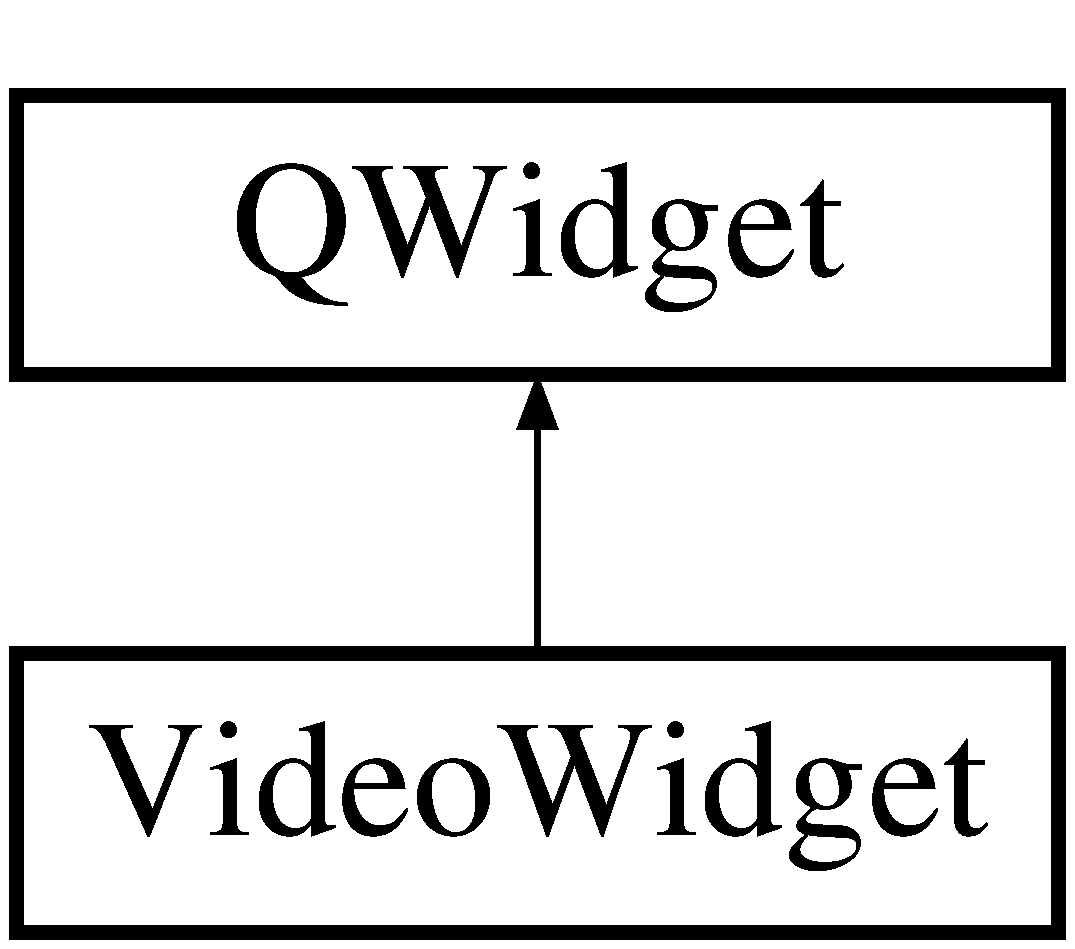
\includegraphics[height=2.000000cm]{classVideoWidget}
\end{center}
\end{figure}
\subsection*{Signals}
\begin{DoxyCompactItemize}
\item 
void \hyperlink{classVideoWidget_aa991152a3b4daee62a7a651cfb06fcf0}{resized} ()
\end{DoxyCompactItemize}
\subsection*{Public Member Functions}
\begin{DoxyCompactItemize}
\item 
\hyperlink{classVideoWidget_a31e7897e4abd9733d45753e4a2e25882}{Video\+Widget} (Q\+Widget $\ast$parent=0)
\item 
\hyperlink{classVideoWidget_a77b8af4076f462cb5db7932e88d46829}{$\sim$\+Video\+Widget} ()
\item 
void \hyperlink{classVideoWidget_a535271277b91deed6d52cb1d11caf80d}{resize\+Event} (Q\+Resize\+Event $\ast$event)
\end{DoxyCompactItemize}


\subsection{Detailed Description}


Definition at line 12 of file videowidget.\+h.



\subsection{Constructor \& Destructor Documentation}
\hypertarget{classVideoWidget_a31e7897e4abd9733d45753e4a2e25882}{}\index{Video\+Widget@{Video\+Widget}!Video\+Widget@{Video\+Widget}}
\index{Video\+Widget@{Video\+Widget}!Video\+Widget@{Video\+Widget}}
\subsubsection[{Video\+Widget}]{\setlength{\rightskip}{0pt plus 5cm}Video\+Widget\+::\+Video\+Widget (
\begin{DoxyParamCaption}
\item[{Q\+Widget $\ast$}]{parent = {\ttfamily 0}}
\end{DoxyParamCaption}
)\hspace{0.3cm}{\ttfamily [explicit]}}\label{classVideoWidget_a31e7897e4abd9733d45753e4a2e25882}
Constructor 
\begin{DoxyParams}{Parameters}
{\em parent} & Parent widget \\
\hline
\end{DoxyParams}


Definition at line 9 of file videowidget.\+cpp.

\hypertarget{classVideoWidget_a77b8af4076f462cb5db7932e88d46829}{}\index{Video\+Widget@{Video\+Widget}!````~Video\+Widget@{$\sim$\+Video\+Widget}}
\index{````~Video\+Widget@{$\sim$\+Video\+Widget}!Video\+Widget@{Video\+Widget}}
\subsubsection[{$\sim$\+Video\+Widget}]{\setlength{\rightskip}{0pt plus 5cm}Video\+Widget\+::$\sim$\+Video\+Widget (
\begin{DoxyParamCaption}
{}
\end{DoxyParamCaption}
)}\label{classVideoWidget_a77b8af4076f462cb5db7932e88d46829}
Destructor 

Definition at line 14 of file videowidget.\+cpp.



\subsection{Member Function Documentation}
\hypertarget{classVideoWidget_aa991152a3b4daee62a7a651cfb06fcf0}{}\index{Video\+Widget@{Video\+Widget}!resized@{resized}}
\index{resized@{resized}!Video\+Widget@{Video\+Widget}}
\subsubsection[{resized}]{\setlength{\rightskip}{0pt plus 5cm}void Video\+Widget\+::resized (
\begin{DoxyParamCaption}
{}
\end{DoxyParamCaption}
)\hspace{0.3cm}{\ttfamily [signal]}}\label{classVideoWidget_aa991152a3b4daee62a7a651cfb06fcf0}
This signal is emitted when the widget is resized. \hypertarget{classVideoWidget_a535271277b91deed6d52cb1d11caf80d}{}\index{Video\+Widget@{Video\+Widget}!resize\+Event@{resize\+Event}}
\index{resize\+Event@{resize\+Event}!Video\+Widget@{Video\+Widget}}
\subsubsection[{resize\+Event}]{\setlength{\rightskip}{0pt plus 5cm}void Video\+Widget\+::resize\+Event (
\begin{DoxyParamCaption}
\item[{Q\+Resize\+Event $\ast$}]{event}
\end{DoxyParamCaption}
)}\label{classVideoWidget_a535271277b91deed6d52cb1d11caf80d}
When the widget is resized, the \hyperlink{classVideoWidget_aa991152a3b4daee62a7a651cfb06fcf0}{resized()} signal is emitted. 
\begin{DoxyParams}{Parameters}
{\em event} & \\
\hline
\end{DoxyParams}


Definition at line 19 of file videowidget.\+cpp.



The documentation for this class was generated from the following files\+:\begin{DoxyCompactItemize}
\item 
headers/videowidget.\+h\item 
sources/\hyperlink{videowidget_8cpp}{videowidget.\+cpp}\end{DoxyCompactItemize}

\chapter{File Documentation}
\hypertarget{anchoritem_8h}{}\section{headers/anchoritem.h File Reference}
\label{anchoritem_8h}\index{headers/anchoritem.\+h@{headers/anchoritem.\+h}}
{\ttfamily \#include $<$Q\+Widget$>$}\\*
{\ttfamily \#include $<$Q\+Label$>$}\\*
{\ttfamily \#include $<$Q\+H\+Box\+Layout$>$}\\*
{\ttfamily \#include \char`\"{}timelabel.\+h\char`\"{}}\\*
{\ttfamily \#include $<$stdint.\+h$>$}\\*
\subsection*{Classes}
\begin{DoxyCompactItemize}
\item 
class \hyperlink{classAnchorItem}{Anchor\+Item}
\end{DoxyCompactItemize}
\subsection*{Enumerations}
\begin{DoxyCompactItemize}
\item 
\hypertarget{anchoritem_8h_aee432dcb83a6f7c488d7835165f26a78}{}enum {\bfseries Item\+Type} \+: int \{ {\bfseries B\+E\+G\+I\+N\+N\+I\+N\+G}, 
{\bfseries E\+N\+D}, 
{\bfseries C\+H\+A\+N\+G\+E}
 \}\label{anchoritem_8h_aee432dcb83a6f7c488d7835165f26a78}

\end{DoxyCompactItemize}


\subsection{Detailed Description}
\begin{DoxyAuthor}{Author}
Martin Borek (\href{mailto:mborekcz@gmail.com}{\tt mborekcz@gmail.\+com}) 
\end{DoxyAuthor}
\begin{DoxyDate}{Date}
May, 2015 
\end{DoxyDate}

\hypertarget{avwriter_8h}{}\section{headers/avwriter.h File Reference}
\label{avwriter_8h}\index{headers/avwriter.\+h@{headers/avwriter.\+h}}
{\ttfamily \#include $<$libavcodec/avcodec.\+h$>$}\\*
{\ttfamily \#include $<$libavformat/avformat.\+h$>$}\\*
{\ttfamily \#include $<$libswscale/swscale.\+h$>$}\\*
{\ttfamily \#include $<$libavutil/common.\+h$>$}\\*
{\ttfamily \#include $<$libavutil/imgutils.\+h$>$}\\*
{\ttfamily \#include $<$libavutil/mathematics.\+h$>$}\\*
{\ttfamily \#include $<$libavutil/samplefmt.\+h$>$}\\*
{\ttfamily \#include $<$libavutil/avassert.\+h$>$}\\*
{\ttfamily \#include $<$libavutil/channel\+\_\+layout.\+h$>$}\\*
{\ttfamily \#include $<$libavutil/opt.\+h$>$}\\*
{\ttfamily \#include $<$libavutil/timestamp.\+h$>$}\\*
{\ttfamily \#include $<$libswresample/swresample.\+h$>$}\\*
{\ttfamily \#include \char`\"{}videoframe.\+h\char`\"{}}\\*
\subsection*{Classes}
\begin{DoxyCompactItemize}
\item 
class \hyperlink{classAVWriter}{A\+V\+Writer}
\end{DoxyCompactItemize}


\subsection{Detailed Description}
\begin{DoxyAuthor}{Author}
Martin Borek (\href{mailto:mborekcz@gmail.com}{\tt mborekcz@gmail.\+com}) 
\end{DoxyAuthor}
\begin{DoxyDate}{Date}
May, 2015 
\end{DoxyDate}

\hypertarget{colors_8h}{}\section{headers/colors.h File Reference}
\label{colors_8h}\index{headers/colors.\+h@{headers/colors.\+h}}
\subsection*{Classes}
\begin{DoxyCompactItemize}
\item 
class \hyperlink{classColors}{Colors}
\end{DoxyCompactItemize}


\subsection{Detailed Description}
\begin{DoxyAuthor}{Author}
Martin Borek (\href{mailto:mborekcz@gmail.com}{\tt mborekcz@gmail.\+com}) 
\end{DoxyAuthor}
\begin{DoxyDate}{Date}
May, 2015 
\end{DoxyDate}

\hypertarget{ffmpegplayer_8h}{}\section{headers/ffmpegplayer.h File Reference}
\label{ffmpegplayer_8h}\index{headers/ffmpegplayer.\+h@{headers/ffmpegplayer.\+h}}
{\ttfamily \#include $<$string$>$}\\*
{\ttfamily \#include \char`\"{}videoframe.\+h\char`\"{}}\\*
{\ttfamily \#include $<$Q\+Application$>$}\\*
{\ttfamily \#include $<$Q\+Progress\+Dialog$>$}\\*
{\ttfamily \#include $<$cv.\+h$>$}\\*
{\ttfamily \#include $<$cvaux.\+h$>$}\\*
{\ttfamily \#include $<$cxcore.\+h$>$}\\*
{\ttfamily \#include $<$highgui.\+h$>$}\\*
{\ttfamily \#include $<$libavcodec/avcodec.\+h$>$}\\*
{\ttfamily \#include $<$libavformat/avformat.\+h$>$}\\*
{\ttfamily \#include $<$libswscale/swscale.\+h$>$}\\*
{\ttfamily \#include $<$libavutil/common.\+h$>$}\\*
{\ttfamily \#include $<$libavutil/imgutils.\+h$>$}\\*
{\ttfamily \#include $<$libavutil/mathematics.\+h$>$}\\*
{\ttfamily \#include $<$libavutil/samplefmt.\+h$>$}\\*
{\ttfamily \#include $<$libavutil/avassert.\+h$>$}\\*
{\ttfamily \#include $<$libavutil/channel\+\_\+layout.\+h$>$}\\*
{\ttfamily \#include $<$libavutil/opt.\+h$>$}\\*
{\ttfamily \#include $<$libavutil/timestamp.\+h$>$}\\*
{\ttfamily \#include $<$libswresample/swresample.\+h$>$}\\*
\subsection*{Classes}
\begin{DoxyCompactItemize}
\item 
struct \hyperlink{structOpenException}{Open\+Exception}
\item 
struct \hyperlink{structUserCanceledOpeningException}{User\+Canceled\+Opening\+Exception}
\item 
class \hyperlink{classFFmpegPlayer}{F\+Fmpeg\+Player}
\end{DoxyCompactItemize}


\subsection{Detailed Description}
\begin{DoxyAuthor}{Author}
Martin Borek (\href{mailto:mborekcz@gmail.com}{\tt mborekcz@gmail.\+com}) 
\end{DoxyAuthor}
\begin{DoxyDate}{Date}
May, 2015 
\end{DoxyDate}

\hypertarget{helpbrowser_8h}{}\section{headers/helpbrowser.h File Reference}
\label{helpbrowser_8h}\index{headers/helpbrowser.\+h@{headers/helpbrowser.\+h}}
{\ttfamily \#include $<$Q\+Text\+Browser$>$}\\*
{\ttfamily \#include $<$Q\+Help\+Engine$>$}\\*
{\ttfamily \#include $<$Q\+Widget$>$}\\*
\subsection*{Classes}
\begin{DoxyCompactItemize}
\item 
class \hyperlink{classHelpBrowser}{Help\+Browser}
\end{DoxyCompactItemize}


\subsection{Detailed Description}
\begin{DoxyAuthor}{Author}
Martin Borek (\href{mailto:mborekcz@gmail.com}{\tt mborekcz@gmail.\+com}) 
\end{DoxyAuthor}
\begin{DoxyDate}{Date}
May, 2015 
\end{DoxyDate}

\hypertarget{imagelabel_8h}{}\section{headers/imagelabel.h File Reference}
\label{imagelabel_8h}\index{headers/imagelabel.\+h@{headers/imagelabel.\+h}}
{\ttfamily \#include \char`\"{}selection.\+h\char`\"{}}\\*
{\ttfamily \#include $<$Q\+Label$>$}\\*
{\ttfamily \#include $<$Q\+Mouse\+Event$>$}\\*
\subsection*{Classes}
\begin{DoxyCompactItemize}
\item 
class \hyperlink{classImageLabel}{Image\+Label}
\end{DoxyCompactItemize}


\subsection{Detailed Description}
\begin{DoxyAuthor}{Author}
Martin Borek (\href{mailto:mborekcz@gmail.com}{\tt mborekcz@gmail.\+com}) 
\end{DoxyAuthor}
\begin{DoxyDate}{Date}
May, 2015 
\end{DoxyDate}

\hypertarget{mainwindow_8h}{}\section{headers/mainwindow.h File Reference}
\label{mainwindow_8h}\index{headers/mainwindow.\+h@{headers/mainwindow.\+h}}
{\ttfamily \#include $<$Q\+Main\+Window$>$}\\*
{\ttfamily \#include $<$Q\+File\+Info$>$}\\*
{\ttfamily \#include $<$Q\+List\+Widget\+Item$>$}\\*
{\ttfamily \#include $<$Q\+Settings$>$}\\*
{\ttfamily \#include $<$Q\+Help\+Engine$>$}\\*
{\ttfamily \#include \char`\"{}imagelabel.\+h\char`\"{}}\\*
{\ttfamily \#include \char`\"{}timelabel.\+h\char`\"{}}\\*
{\ttfamily \#include \char`\"{}videotracker.\+h\char`\"{}}\\*
{\ttfamily \#include \char`\"{}anchoritem.\+h\char`\"{}}\\*
{\ttfamily \#include \char`\"{}trajectoryitem.\+h\char`\"{}}\\*
{\ttfamily \#include $<$cereal/types/string.\+hpp$>$}\\*
{\ttfamily \#include $<$cereal/types/map.\+hpp$>$}\\*
{\ttfamily \#include $<$cereal/types/utility.\+hpp$>$}\\*
\subsection*{Classes}
\begin{DoxyCompactItemize}
\item 
class \hyperlink{classMainWindow}{Main\+Window}
\end{DoxyCompactItemize}
\subsection*{Enumerations}
\begin{DoxyCompactItemize}
\item 
\hypertarget{mainwindow_8h_a65b233b9306f23f5a4a8668a879a8316}{}enum {\bfseries Selection\+State} \+: int \{ \\*
{\bfseries N\+O\+\_\+\+S\+E\+L\+E\+C\+T\+I\+O\+N}, 
{\bfseries N\+E\+W\+\_\+\+O\+B\+J\+E\+C\+T}, 
{\bfseries C\+H\+A\+N\+G\+E\+\_\+\+P\+O\+S\+I\+T\+I\+O\+N}, 
{\bfseries S\+E\+T\+\_\+\+E\+N\+D\+\_\+\+F\+R\+A\+M\+E}, 
\\*
{\bfseries N\+E\+W\+\_\+\+S\+E\+C\+T\+I\+O\+N}
 \}\label{mainwindow_8h_a65b233b9306f23f5a4a8668a879a8316}

\end{DoxyCompactItemize}


\subsection{Detailed Description}
\begin{DoxyAuthor}{Author}
Martin Borek (\href{mailto:mborekcz@gmail.com}{\tt mborekcz@gmail.\+com}) 
\end{DoxyAuthor}
\begin{DoxyDate}{Date}
May, 2015 
\end{DoxyDate}

\hypertarget{objectshape_8h}{}\section{headers/objectshape.h File Reference}
\label{objectshape_8h}\index{headers/objectshape.\+h@{headers/objectshape.\+h}}
\subsection*{Classes}
\begin{DoxyCompactItemize}
\item 
struct \hyperlink{structObjectShape}{Object\+Shape}
\end{DoxyCompactItemize}


\subsection{Detailed Description}
\begin{DoxyAuthor}{Author}
Martin Borek (\href{mailto:mborekcz@gmail.com}{\tt mborekcz@gmail.\+com}) 
\end{DoxyAuthor}
\begin{DoxyDate}{Date}
May, 2015 
\end{DoxyDate}

\hypertarget{playerslider_8h}{}\section{headers/playerslider.h File Reference}
\label{playerslider_8h}\index{headers/playerslider.\+h@{headers/playerslider.\+h}}
{\ttfamily \#include $<$Q\+Slider$>$}\\*
{\ttfamily \#include $<$Q\+Mouse\+Event$>$}\\*
\subsection*{Classes}
\begin{DoxyCompactItemize}
\item 
class \hyperlink{classPlayerSlider}{Player\+Slider}
\end{DoxyCompactItemize}


\subsection{Detailed Description}
\begin{DoxyAuthor}{Author}
Martin Borek (\href{mailto:mborekcz@gmail.com}{\tt mborekcz@gmail.\+com}) 
\end{DoxyAuthor}
\begin{DoxyDate}{Date}
May, 2015 
\end{DoxyDate}

\hypertarget{selection_8h}{}\section{headers/selection.h File Reference}
\label{selection_8h}\index{headers/selection.\+h@{headers/selection.\+h}}
{\ttfamily \#include $<$objectshape.\+h$>$}\\*
{\ttfamily \#include $<$colors.\+h$>$}\\*
{\ttfamily \#include $<$cereal/types/utility.\+hpp$>$}\\*
\subsection*{Classes}
\begin{DoxyCompactItemize}
\item 
struct \hyperlink{structSelection}{Selection}
\item 
struct \hyperlink{structObjectColor}{Object\+Color}
\item 
struct \hyperlink{structCharacteristics}{Characteristics}
\end{DoxyCompactItemize}


\subsection{Detailed Description}
\begin{DoxyAuthor}{Author}
Martin Borek (\href{mailto:mborekcz@gmail.com}{\tt mborekcz@gmail.\+com}) 
\end{DoxyAuthor}
\begin{DoxyDate}{Date}
May, 2015 
\end{DoxyDate}

\hypertarget{timelabel_8h}{}\section{headers/timelabel.h File Reference}
\label{timelabel_8h}\index{headers/timelabel.\+h@{headers/timelabel.\+h}}
{\ttfamily \#include $<$Q\+Label$>$}\\*
\subsection*{Classes}
\begin{DoxyCompactItemize}
\item 
struct \hyperlink{structTimeConversion_1_1Time}{Time\+Conversion\+::\+Time}
\item 
class \hyperlink{classTimeLabel}{Time\+Label}
\end{DoxyCompactItemize}
\subsection*{Functions}
\begin{DoxyCompactItemize}
\item 
\hypertarget{namespaceTimeConversion_a21859a84f2bf6744d5c3d11209b1d7dd}{}void {\bfseries Time\+Conversion\+::convert\+\_\+time} (\hyperlink{structTimeConversion_1_1Time}{Time} \&converted)\label{namespaceTimeConversion_a21859a84f2bf6744d5c3d11209b1d7dd}

\item 
\hypertarget{namespaceTimeConversion_a7bfb90b27045fcd7842f4ac65a92c4d9}{}void {\bfseries Time\+Conversion\+::\+Time2\+Q\+String} (\hyperlink{structTimeConversion_1_1Time}{Time} const \&time, Q\+String \&time\+String, bool show\+Hours)\label{namespaceTimeConversion_a7bfb90b27045fcd7842f4ac65a92c4d9}

\end{DoxyCompactItemize}


\subsection{Detailed Description}
\begin{DoxyAuthor}{Author}
Martin Borek (\href{mailto:mborekcz@gmail.com}{\tt mborekcz@gmail.\+com}) 
\end{DoxyAuthor}
\begin{DoxyDate}{Date}
May, 2015 
\end{DoxyDate}

\hypertarget{trackedobject_8h}{}\section{headers/trackedobject.h File Reference}
\label{trackedobject_8h}\index{headers/trackedobject.\+h@{headers/trackedobject.\+h}}
{\ttfamily \#include \char`\"{}trackingalgorithm.\+h\char`\"{}}\\*
{\ttfamily \#include \char`\"{}videoframe.\+h\char`\"{}}\\*
{\ttfamily \#include \char`\"{}selection.\+h\char`\"{}}\\*
{\ttfamily \#include $<$Q\+Debug$>$}\\*
{\ttfamily \#include $<$cereal/types/string.\+hpp$>$}\\*
{\ttfamily \#include $<$cereal/types/map.\+hpp$>$}\\*
{\ttfamily \#include $<$cereal/types/tuple.\+hpp$>$}\\*
{\ttfamily \#include $<$cv.\+h$>$}\\*
{\ttfamily \#include $<$cvaux.\+h$>$}\\*
{\ttfamily \#include $<$cxcore.\+h$>$}\\*
{\ttfamily \#include $<$highgui.\+h$>$}\\*
\subsection*{Classes}
\begin{DoxyCompactItemize}
\item 
struct \hyperlink{structTrajectorySection}{Trajectory\+Section}
\item 
struct \hyperlink{structTrajectoryEntry}{Trajectory\+Entry}
\item 
class \hyperlink{classTrackedObject}{Tracked\+Object}
\end{DoxyCompactItemize}


\subsection{Detailed Description}
\begin{DoxyAuthor}{Author}
Martin Borek (\href{mailto:mborekcz@gmail.com}{\tt mborekcz@gmail.\+com}) 
\end{DoxyAuthor}
\begin{DoxyDate}{Date}
May, 2015 
\end{DoxyDate}

\hypertarget{trackingalgorithm_8h}{}\section{headers/trackingalgorithm.h File Reference}
\label{trackingalgorithm_8h}\index{headers/trackingalgorithm.\+h@{headers/trackingalgorithm.\+h}}
{\ttfamily \#include \char`\"{}selection.\+h\char`\"{}}\\*
{\ttfamily \#include $<$cv.\+h$>$}\\*
{\ttfamily \#include $<$cvaux.\+h$>$}\\*
{\ttfamily \#include $<$cxcore.\+h$>$}\\*
{\ttfamily \#include $<$highgui.\+h$>$}\\*
\subsection*{Classes}
\begin{DoxyCompactItemize}
\item 
class \hyperlink{classTrackingAlgorithm}{Tracking\+Algorithm}
\end{DoxyCompactItemize}


\subsection{Detailed Description}
\begin{DoxyAuthor}{Author}
Martin Borek (\href{mailto:mborekcz@gmail.com}{\tt mborekcz@gmail.\+com}) 
\end{DoxyAuthor}
\begin{DoxyDate}{Date}
May, 2015 
\end{DoxyDate}

\hypertarget{trajectoryitem_8h}{}\section{headers/trajectoryitem.h File Reference}
\label{trajectoryitem_8h}\index{headers/trajectoryitem.\+h@{headers/trajectoryitem.\+h}}
{\ttfamily \#include $<$Q\+Widget$>$}\\*
{\ttfamily \#include $<$Q\+Label$>$}\\*
{\ttfamily \#include $<$Q\+H\+Box\+Layout$>$}\\*
{\ttfamily \#include \char`\"{}timelabel.\+h\char`\"{}}\\*
{\ttfamily \#include \char`\"{}selection.\+h\char`\"{}}\\*
{\ttfamily \#include $<$stdint.\+h$>$}\\*
\subsection*{Classes}
\begin{DoxyCompactItemize}
\item 
class \hyperlink{classTrajectoryItem}{Trajectory\+Item}
\end{DoxyCompactItemize}


\subsection{Detailed Description}
\begin{DoxyAuthor}{Author}
Martin Borek (\href{mailto:mborekcz@gmail.com}{\tt mborekcz@gmail.\+com}) 
\end{DoxyAuthor}
\begin{DoxyDate}{Date}
May, 2015 
\end{DoxyDate}

\hypertarget{videoframe_8h}{}\section{headers/videoframe.h File Reference}
\label{videoframe_8h}\index{headers/videoframe.\+h@{headers/videoframe.\+h}}
{\ttfamily \#include $<$cv.\+h$>$}\\*
{\ttfamily \#include $<$cvaux.\+h$>$}\\*
{\ttfamily \#include $<$cxcore.\+h$>$}\\*
{\ttfamily \#include $<$highgui.\+h$>$}\\*
{\ttfamily \#include $<$libavcodec/avcodec.\+h$>$}\\*
{\ttfamily \#include $<$libavformat/avformat.\+h$>$}\\*
{\ttfamily \#include $<$libswscale/swscale.\+h$>$}\\*
\subsection*{Classes}
\begin{DoxyCompactItemize}
\item 
class \hyperlink{classVideoFrame}{Video\+Frame}
\end{DoxyCompactItemize}
\subsection*{Macros}
\begin{DoxyCompactItemize}
\item 
\hypertarget{videoframe_8h_aa7853e7d7eca0c821607b5fef3ca7da5}{}\#define {\bfseries V\+I\+D\+E\+O\+T\+R\+A\+C\+K\+I\+N\+G\+\_\+\+D\+E\+F\+A\+U\+L\+T\+\_\+\+S\+C\+A\+L\+I\+N\+G\+\_\+\+M\+E\+T\+H\+O\+D}~S\+W\+S\+\_\+\+B\+I\+L\+I\+N\+E\+A\+R\label{videoframe_8h_aa7853e7d7eca0c821607b5fef3ca7da5}

\item 
\hypertarget{videoframe_8h_a4713b012a5f898966560d70c34a1c6fb}{}\#define {\bfseries V\+I\+D\+E\+O\+T\+R\+A\+C\+K\+I\+N\+G\+\_\+\+O\+U\+T\+P\+U\+T\+\_\+\+F\+O\+R\+M\+A\+T}~A\+V\+\_\+\+P\+I\+X\+\_\+\+F\+M\+T\+\_\+\+Y\+U\+V420\+P\label{videoframe_8h_a4713b012a5f898966560d70c34a1c6fb}

\end{DoxyCompactItemize}


\subsection{Detailed Description}
\begin{DoxyAuthor}{Author}
Martin Borek (\href{mailto:mborekcz@gmail.com}{\tt mborekcz@gmail.\+com}) 
\end{DoxyAuthor}
\begin{DoxyDate}{Date}
May, 2015 
\end{DoxyDate}

\hypertarget{videotracker_8h}{}\section{headers/videotracker.h File Reference}
\label{videotracker_8h}\index{headers/videotracker.\+h@{headers/videotracker.\+h}}
{\ttfamily \#include $<$cv.\+h$>$}\\*
{\ttfamily \#include $<$cvaux.\+h$>$}\\*
{\ttfamily \#include $<$cxcore.\+h$>$}\\*
{\ttfamily \#include $<$highgui.\+h$>$}\\*
{\ttfamily \#include $<$Q\+Object$>$}\\*
{\ttfamily \#include $<$Q\+Progress\+Dialog$>$}\\*
{\ttfamily \#include $<$Q\+Application$>$}\\*
{\ttfamily \#include $<$memory$>$}\\*
{\ttfamily \#include \char`\"{}ffmpegplayer.\+h\char`\"{}}\\*
{\ttfamily \#include \char`\"{}trackingalgorithm.\+h\char`\"{}}\\*
{\ttfamily \#include \char`\"{}trackedobject.\+h\char`\"{}}\\*
{\ttfamily \#include \char`\"{}videoframe.\+h\char`\"{}}\\*
{\ttfamily \#include \char`\"{}selection.\+h\char`\"{}}\\*
{\ttfamily \#include $<$cereal/types/vector.\+hpp$>$}\\*
{\ttfamily \#include $<$cereal/types/memory.\+hpp$>$}\\*
\subsection*{Classes}
\begin{DoxyCompactItemize}
\item 
struct \hyperlink{structOutputException}{Output\+Exception}
\item 
struct \hyperlink{structUserCanceledException}{User\+Canceled\+Exception}
\item 
class \hyperlink{classVideoTracker}{Video\+Tracker}
\end{DoxyCompactItemize}


\subsection{Detailed Description}
\begin{DoxyAuthor}{Author}
Martin Borek (\href{mailto:mborekcz@gmail.com}{\tt mborekcz@gmail.\+com}) 
\end{DoxyAuthor}
\begin{DoxyDate}{Date}
May, 2015 
\end{DoxyDate}

\hypertarget{anchoritem_8cpp}{}\section{sources/anchoritem.cpp File Reference}
\label{anchoritem_8cpp}\index{sources/anchoritem.\+cpp@{sources/anchoritem.\+cpp}}
{\ttfamily \#include \char`\"{}anchoritem.\+h\char`\"{}}\\*
{\ttfamily \#include $<$Q\+Debug$>$}\\*
{\ttfamily \#include $<$Q\+Mouse\+Event$>$}\\*


\subsection{Detailed Description}
\begin{DoxyAuthor}{Author}
Martin Borek (\href{mailto:mborekcz@gmail.com}{\tt mborekcz@gmail.\+com}) 
\end{DoxyAuthor}
\begin{DoxyDate}{Date}
May, 2015 
\end{DoxyDate}

\hypertarget{avwriter_8cpp}{}\section{sources/avwriter.cpp File Reference}
\label{avwriter_8cpp}\index{sources/avwriter.\+cpp@{sources/avwriter.\+cpp}}
{\ttfamily \#include \char`\"{}avwriter.\+h\char`\"{}}\\*
{\ttfamily \#include $<$Q\+Debug$>$}\\*
{\ttfamily \#include $<$cassert$>$}\\*


\subsection{Detailed Description}
\begin{DoxyAuthor}{Author}
Martin Borek (\href{mailto:mborekcz@gmail.com}{\tt mborekcz@gmail.\+com}) 
\end{DoxyAuthor}
\begin{DoxyDate}{Date}
May, 2015 
\end{DoxyDate}

\hypertarget{colors_8cpp}{}\section{sources/colors.cpp File Reference}
\label{colors_8cpp}\index{sources/colors.\+cpp@{sources/colors.\+cpp}}
{\ttfamily \#include \char`\"{}colors.\+h\char`\"{}}\\*


\subsection{Detailed Description}
\begin{DoxyAuthor}{Author}
Martin Borek (\href{mailto:mborekcz@gmail.com}{\tt mborekcz@gmail.\+com}) 
\end{DoxyAuthor}
\begin{DoxyDate}{Date}
May, 2015 
\end{DoxyDate}

\hypertarget{ffmpegplayer_8cpp}{}\section{sources/ffmpegplayer.cpp File Reference}
\label{ffmpegplayer_8cpp}\index{sources/ffmpegplayer.\+cpp@{sources/ffmpegplayer.\+cpp}}
{\ttfamily \#include \char`\"{}ffmpegplayer.\+h\char`\"{}}\\*
{\ttfamily \#include $<$Q\+Debug$>$}\\*
{\ttfamily \#include $<$cassert$>$}\\*
\subsection*{Macros}
\begin{DoxyCompactItemize}
\item 
\hypertarget{ffmpegplayer_8cpp_a8d9c9326b9da92a70fd57a19dba00c45}{}\#define {\bfseries V\+I\+D\+E\+O\+T\+R\+A\+C\+K\+I\+N\+G\+\_\+\+M\+S2\+D\+U\+R\+A\+T\+I\+O\+N}~1000\label{ffmpegplayer_8cpp_a8d9c9326b9da92a70fd57a19dba00c45}

\item 
\hypertarget{ffmpegplayer_8cpp_a578f1108c3c17b3fb4d6ec11b11cbd39}{}\#define {\bfseries V\+I\+D\+E\+O\+T\+R\+A\+C\+K\+I\+N\+G\+\_\+\+T\+I\+M\+E\+\_\+\+B\+A\+S\+E\+\_\+\+Q}~A\+V\+Rational\{1, A\+V\+\_\+\+T\+I\+M\+E\+\_\+\+B\+A\+S\+E\}\label{ffmpegplayer_8cpp_a578f1108c3c17b3fb4d6ec11b11cbd39}

\item 
\hypertarget{ffmpegplayer_8cpp_a7f6ec3438aec3becf6510df57cd2a660}{}\#define {\bfseries V\+I\+D\+E\+O\+T\+R\+A\+C\+K\+I\+N\+G\+\_\+\+M\+S\+\_\+\+T\+I\+M\+E\+\_\+\+B\+A\+S\+E\+\_\+\+Q}~A\+V\+Rational\{1, 1000\}\label{ffmpegplayer_8cpp_a7f6ec3438aec3becf6510df57cd2a660}

\end{DoxyCompactItemize}


\subsection{Detailed Description}
\begin{DoxyAuthor}{Author}
Martin Borek (\href{mailto:mborekcz@gmail.com}{\tt mborekcz@gmail.\+com}) 
\end{DoxyAuthor}
\begin{DoxyDate}{Date}
May, 2015 
\end{DoxyDate}

\hypertarget{helpbrowser_8cpp}{}\section{sources/helpbrowser.cpp File Reference}
\label{helpbrowser_8cpp}\index{sources/helpbrowser.\+cpp@{sources/helpbrowser.\+cpp}}
{\ttfamily \#include \char`\"{}helpbrowser.\+h\char`\"{}}\\*


\subsection{Detailed Description}
\begin{DoxyAuthor}{Author}
Martin Borek (\href{mailto:mborekcz@gmail.com}{\tt mborekcz@gmail.\+com}) 
\end{DoxyAuthor}
\begin{DoxyDate}{Date}
May, 2015 
\end{DoxyDate}

\hypertarget{imagelabel_8cpp}{}\section{sources/imagelabel.cpp File Reference}
\label{imagelabel_8cpp}\index{sources/imagelabel.\+cpp@{sources/imagelabel.\+cpp}}
{\ttfamily \#include \char`\"{}imagelabel.\+h\char`\"{}}\\*
{\ttfamily \#include $<$Qt\+Debug$>$}\\*
{\ttfamily \#include $<$Q\+Painter$>$}\\*
{\ttfamily \#include $<$cassert$>$}\\*


\subsection{Detailed Description}
\begin{DoxyAuthor}{Author}
Martin Borek (\href{mailto:mborekcz@gmail.com}{\tt mborekcz@gmail.\+com}) 
\end{DoxyAuthor}
\begin{DoxyDate}{Date}
May, 2015 
\end{DoxyDate}

\hypertarget{main_8cpp}{}\section{sources/main.cpp File Reference}
\label{main_8cpp}\index{sources/main.\+cpp@{sources/main.\+cpp}}
{\ttfamily \#include \char`\"{}mainwindow.\+h\char`\"{}}\\*
{\ttfamily \#include $<$Q\+Application$>$}\\*
\subsection*{Functions}
\begin{DoxyCompactItemize}
\item 
\hypertarget{main_8cpp_a0ddf1224851353fc92bfbff6f499fa97}{}int {\bfseries main} (int argc, char $\ast$argv\mbox{[}$\,$\mbox{]})\label{main_8cpp_a0ddf1224851353fc92bfbff6f499fa97}

\end{DoxyCompactItemize}


\subsection{Detailed Description}
\begin{DoxyAuthor}{Author}
Martin Borek (\href{mailto:mborekcz@gmail.com}{\tt mborekcz@gmail.\+com}) 
\end{DoxyAuthor}
\begin{DoxyDate}{Date}
May, 2015 
\end{DoxyDate}

\hypertarget{mainwindow_8cpp}{}\section{sources/mainwindow.cpp File Reference}
\label{mainwindow_8cpp}\index{sources/mainwindow.\+cpp@{sources/mainwindow.\+cpp}}
{\ttfamily \#include \char`\"{}mainwindow.\+h\char`\"{}}\\*
{\ttfamily \#include \char`\"{}ui\+\_\+mainwindow.\+h\char`\"{}}\\*
{\ttfamily \#include \char`\"{}selection.\+h\char`\"{}}\\*
{\ttfamily \#include \char`\"{}colors.\+h\char`\"{}}\\*
{\ttfamily \#include \char`\"{}objectshape.\+h\char`\"{}}\\*
{\ttfamily \#include $<$cereal/archives/json.\+hpp$>$}\\*
{\ttfamily \#include $<$cereal/archives/xml.\+hpp$>$}\\*
{\ttfamily \#include $<$utility$>$}\\*
{\ttfamily \#include $<$fstream$>$}\\*
{\ttfamily \#include $<$Qt\+Gui$>$}\\*
{\ttfamily \#include $<$Q\+Debug$>$}\\*
{\ttfamily \#include $<$Q\+File\+Dialog$>$}\\*
{\ttfamily \#include $<$Q\+Painter$>$}\\*
{\ttfamily \#include $<$Q\+Progress\+Dialog$>$}\\*
{\ttfamily \#include $<$Q\+Input\+Dialog$>$}\\*
{\ttfamily \#include $<$Q\+Color\+Dialog$>$}\\*
{\ttfamily \#include $<$Q\+Message\+Box$>$}\\*
{\ttfamily \#include $<$Q\+Menu$>$}\\*
{\ttfamily \#include $<$Q\+Translator$>$}\\*
{\ttfamily \#include $<$Q\+Splitter$>$}\\*
{\ttfamily \#include $<$Q\+Dock\+Widget$>$}\\*
{\ttfamily \#include $<$helpbrowser.\+h$>$}\\*
\subsection*{Macros}
\begin{DoxyCompactItemize}
\item 
\hypertarget{mainwindow_8cpp_a00702f6f73af9c288e50dccea018f007}{}\#define {\bfseries V\+I\+D\+E\+O\+T\+R\+A\+C\+K\+I\+N\+G\+\_\+10\+M\+S2\+S}~100\label{mainwindow_8cpp_a00702f6f73af9c288e50dccea018f007}

\item 
\hypertarget{mainwindow_8cpp_a2afbb6b3668c5bbc8d052d3b1ea3f6c3}{}\#define {\bfseries V\+I\+D\+E\+O\+T\+R\+A\+C\+K\+I\+N\+G\+\_\+\+T\+I\+M\+E\+R\+\_\+\+C\+O\+N\+S\+T\+A\+N\+T}~1.\+5\label{mainwindow_8cpp_a2afbb6b3668c5bbc8d052d3b1ea3f6c3}

\item 
\hypertarget{mainwindow_8cpp_a8829f65f6815dc499c4fd89563c5954b}{}\#define {\bfseries V\+I\+D\+E\+O\+T\+R\+A\+C\+K\+I\+N\+G\+\_\+\+T\+I\+M\+E\+R\+\_\+\+C\+O\+N\+S\+T\+A\+N\+T\+\_\+\+F\+A\+S\+T}~0.\+5\label{mainwindow_8cpp_a8829f65f6815dc499c4fd89563c5954b}

\item 
\hypertarget{mainwindow_8cpp_a4a34a3bdf7b84f8d9feb137faeb051d6}{}\#define {\bfseries V\+I\+D\+E\+O\+T\+R\+A\+C\+K\+I\+N\+G\+\_\+\+T\+I\+M\+E\+R\+\_\+\+C\+O\+N\+S\+T\+A\+N\+T\+\_\+\+S\+L\+O\+W}~0.\+2\label{mainwindow_8cpp_a4a34a3bdf7b84f8d9feb137faeb051d6}

\end{DoxyCompactItemize}


\subsection{Detailed Description}
\begin{DoxyAuthor}{Author}
Martin Borek (\href{mailto:mborekcz@gmail.com}{\tt mborekcz@gmail.\+com}) 
\end{DoxyAuthor}
\begin{DoxyDate}{Date}
May, 2015 
\end{DoxyDate}

\hypertarget{objectshape_8cpp}{}\section{sources/objectshape.cpp File Reference}
\label{objectshape_8cpp}\index{sources/objectshape.\+cpp@{sources/objectshape.\+cpp}}
{\ttfamily \#include \char`\"{}objectshape.\+h\char`\"{}}\\*


\subsection{Detailed Description}
\begin{DoxyAuthor}{Author}
Martin Borek (\href{mailto:mborekcz@gmail.com}{\tt mborekcz@gmail.\+com}) 
\end{DoxyAuthor}
\begin{DoxyDate}{Date}
May, 2015 
\end{DoxyDate}

\hypertarget{playerslider_8cpp}{}\section{sources/playerslider.cpp File Reference}
\label{playerslider_8cpp}\index{sources/playerslider.\+cpp@{sources/playerslider.\+cpp}}
{\ttfamily \#include \char`\"{}playerslider.\+h\char`\"{}}\\*
{\ttfamily \#include $<$Q\+Debug$>$}\\*


\subsection{Detailed Description}
\begin{DoxyAuthor}{Author}
Martin Borek (\href{mailto:mborekcz@gmail.com}{\tt mborekcz@gmail.\+com}) 
\end{DoxyAuthor}
\begin{DoxyDate}{Date}
May, 2015 
\end{DoxyDate}

\hypertarget{timelabel_8cpp}{}\section{sources/timelabel.cpp File Reference}
\label{timelabel_8cpp}\index{sources/timelabel.\+cpp@{sources/timelabel.\+cpp}}
{\ttfamily \#include \char`\"{}timelabel.\+h\char`\"{}}\\*
{\ttfamily \#include $<$Q\+Debug$>$}\\*


\subsection{Detailed Description}
\begin{DoxyAuthor}{Author}
Martin Borek (\href{mailto:mborekcz@gmail.com}{\tt mborekcz@gmail.\+com}) 
\end{DoxyAuthor}
\begin{DoxyDate}{Date}
May, 2015 
\end{DoxyDate}

\hypertarget{trackedobject_8cpp}{}\section{sources/trackedobject.cpp File Reference}
\label{trackedobject_8cpp}\index{sources/trackedobject.\+cpp@{sources/trackedobject.\+cpp}}
{\ttfamily \#include \char`\"{}trackedobject.\+h\char`\"{}}\\*
{\ttfamily \#include $<$Q\+Debug$>$}\\*
{\ttfamily \#include \char`\"{}objectshape.\+h\char`\"{}}\\*


\subsection{Detailed Description}
\begin{DoxyAuthor}{Author}
Martin Borek (\href{mailto:mborekcz@gmail.com}{\tt mborekcz@gmail.\+com}) 
\end{DoxyAuthor}
\begin{DoxyDate}{Date}
May, 2015 
\end{DoxyDate}

\hypertarget{trackingalgorithm_8cpp}{}\section{sources/trackingalgorithm.cpp File Reference}
\label{trackingalgorithm_8cpp}\index{sources/trackingalgorithm.\+cpp@{sources/trackingalgorithm.\+cpp}}
{\ttfamily \#include \char`\"{}trackingalgorithm.\+h\char`\"{}}\\*
{\ttfamily \#include \char`\"{}opencvx/cvxmat.\+h\char`\"{}}\\*
{\ttfamily \#include \char`\"{}opencvx/cvxrectangle.\+h\char`\"{}}\\*
{\ttfamily \#include \char`\"{}opencvx/cvrect32f.\+h\char`\"{}}\\*
{\ttfamily \#include \char`\"{}opencvx/cvcropimageroi.\+h\char`\"{}}\\*
{\ttfamily \#include \char`\"{}opencvx/cvdrawrectangle.\+h\char`\"{}}\\*
{\ttfamily \#include \char`\"{}opencvx/cvparticle.\+h\char`\"{}}\\*
{\ttfamily \#include \char`\"{}tracking\+\_\+algorithm/observetemplate.\+h\char`\"{}}\\*
{\ttfamily \#include \char`\"{}tracking\+\_\+algorithm/state.\+h\char`\"{}}\\*
{\ttfamily \#include $<$iostream$>$}\\*
\subsection*{Macros}
\begin{DoxyCompactItemize}
\item 
\hypertarget{trackingalgorithm_8cpp_a3da44afeba217135a680a7477b5e3ce3}{}\#define {\bfseries D\+E\+F\+A\+U\+L\+T}~0\label{trackingalgorithm_8cpp_a3da44afeba217135a680a7477b5e3ce3}

\item 
\hypertarget{trackingalgorithm_8cpp_a217af7d1fc87d4eeededa5ecb3ce1e42}{}\#define {\bfseries D\+R\+A\+W\+\_\+\+P\+A\+R\+T\+I\+C\+L\+E\+S\+\_\+\+R\+E\+A\+L\+L\+O\+C}~512\label{trackingalgorithm_8cpp_a217af7d1fc87d4eeededa5ecb3ce1e42}

\end{DoxyCompactItemize}


\subsection{Detailed Description}
\begin{DoxyAuthor}{Author}
Martin Borek (\href{mailto:mborekcz@gmail.com}{\tt mborekcz@gmail.\+com}) 
\end{DoxyAuthor}
\begin{DoxyDate}{Date}
May, 2015 
\end{DoxyDate}

\hypertarget{trajectoryitem_8cpp}{}\section{sources/trajectoryitem.cpp File Reference}
\label{trajectoryitem_8cpp}\index{sources/trajectoryitem.\+cpp@{sources/trajectoryitem.\+cpp}}
{\ttfamily \#include \char`\"{}trajectoryitem.\+h\char`\"{}}\\*
{\ttfamily \#include $<$Q\+Debug$>$}\\*
{\ttfamily \#include $<$Q\+Mouse\+Event$>$}\\*


\subsection{Detailed Description}
\begin{DoxyAuthor}{Author}
Martin Borek (\href{mailto:mborekcz@gmail.com}{\tt mborekcz@gmail.\+com}) 
\end{DoxyAuthor}
\begin{DoxyDate}{Date}
May, 2015 
\end{DoxyDate}

\hypertarget{videoframe_8cpp}{}\section{sources/videoframe.cpp File Reference}
\label{videoframe_8cpp}\index{sources/videoframe.\+cpp@{sources/videoframe.\+cpp}}
{\ttfamily \#include \char`\"{}videoframe.\+h\char`\"{}}\\*
{\ttfamily \#include $<$Q\+Debug$>$}\\*


\subsection{Detailed Description}
\begin{DoxyAuthor}{Author}
Martin Borek (\href{mailto:mborekcz@gmail.com}{\tt mborekcz@gmail.\+com}) 
\end{DoxyAuthor}
\begin{DoxyDate}{Date}
May, 2015 
\end{DoxyDate}

\hypertarget{videotracker_8cpp}{}\section{sources/videotracker.cpp File Reference}
\label{videotracker_8cpp}\index{sources/videotracker.\+cpp@{sources/videotracker.\+cpp}}
{\ttfamily \#include $<$Q\+Image$>$}\\*
{\ttfamily \#include $<$Q\+Debug$>$}\\*
{\ttfamily \#include \char`\"{}videotracker.\+h\char`\"{}}\\*
{\ttfamily \#include \char`\"{}avwriter.\+h\char`\"{}}\\*


\subsection{Detailed Description}
\begin{DoxyAuthor}{Author}
Martin Borek (\href{mailto:mborekcz@gmail.com}{\tt mborekcz@gmail.\+com}) 
\end{DoxyAuthor}
\begin{DoxyDate}{Date}
May, 2015 
\end{DoxyDate}

\hypertarget{videowidget_8cpp}{}\section{sources/videowidget.cpp File Reference}
\label{videowidget_8cpp}\index{sources/videowidget.\+cpp@{sources/videowidget.\+cpp}}
{\ttfamily \#include \char`\"{}videowidget.\+h\char`\"{}}\\*


\subsection{Detailed Description}
\begin{DoxyAuthor}{Author}
Martin Borek (\href{mailto:mborekcz@gmail.com}{\tt mborekcz@gmail.\+com}) 
\end{DoxyAuthor}
\begin{DoxyDate}{Date}
May, 2015 
\end{DoxyDate}

%--- End generated contents ---

% Index
\backmatter
\newpage
\phantomsection
\clearemptydoublepage
\addcontentsline{toc}{chapter}{Index}
\printindex

\end{document}
